\documentclass[8pt]{beamer}

\usetheme{metropolis}

\usepackage{emoji}
\usepackage{pgfplots}
\usepackage{pgfplotstable}
\usepackage{tikz}
\usepackage{transparent}

\usepgfplotslibrary{fillbetween}
\usepgfplotslibrary{groupplots}

\usetikzlibrary{arrows.meta}
\usetikzlibrary{calc}
\usetikzlibrary{matrix}

\date{19.10.23}
\title{PSY2301: The psychology of judgement and decision making}
\subtitle{Artificial Intelligence and decision-making}
\author{Esten H. Leonardsen}

\def\logoheight{1.2cm}
\def\logosep{0.5cm}

\definecolor{headerbackground}{HTML}{23373b}
\definecolor{headerforeground}{HTML}{F4F4F4}
\setbeamercolor{footer}{bg=headerbackground, fg=headerforeground}

\defbeamertemplate*{footline}{mycin}{%
  \leavevmode%
  \hbox{%
  \begin{beamercolorbox}[wd=\paperwidth,ht=2.25ex,dp=1ex,center]{footer}%
	\href{https://www.sciencedirect.com/science/article/pii/S0020737378800492}{MYCIN: a knowledge-based consultation program for infectious disease diagnosis, William van Melle, \textit{International Journal of Man-Machine Studies}, 1978}
  \end{beamercolorbox}%
  }%
  \vskip0pt%
}

\defbeamertemplate*{footline}{backprop}{%
  \leavevmode%
  \hbox{%
  \begin{beamercolorbox}[wd=\paperwidth,ht=2.25ex,dp=1ex,center]{footer}%
	\href{https://www.nature.com/articles/323533a0}{Learning representations by back-propagating errors, Rumelhart, D., Hinton, G. \& Williams, R, \textit{Nature}, 1986}
  \end{beamercolorbox}%
  }%
  \vskip0pt%
}

\defbeamertemplate*{footline}{eliza}{%
  \leavevmode%
  \hbox{%
  \begin{beamercolorbox}[wd=\paperwidth,ht=2.25ex,dp=1ex,center]{footer}%
	\href{https://web.njit.edu/~ronkowit/eliza.html}{ELIZA: a very basic Rogerian psychotherapist chatbot}
  \end{beamercolorbox}%
  }%
  \vskip0pt%
}

\defbeamertemplate*{footline}{neuron}{%
  \leavevmode%
  \hbox{%
  \begin{beamercolorbox}[wd=\paperwidth,ht=2.25ex,dp=1ex,center]{footer}%
	\href{https://opentextbc.ca/introductiontopsychology/chapter/3-1-the-neuron-is-the-building-block-of-the-nervous-system/}{The neuron is the building block of the nervous system}
  \end{beamercolorbox}%
  }%
  \vskip0pt%
}

\defbeamertemplate*{footline}{turing}{%
  \leavevmode%
  \hbox{%
  \begin{beamercolorbox}[wd=\paperwidth,ht=2.25ex,dp=1ex,center]{footer}%
	\href{https://link.springer.com/chapter/10.1007/978-1-4020-6710-5_3}{Computing Machinery and Intelligence, A. M. Turing, \textit{Mind}, 1950.}
  \end{beamercolorbox}%
  }%
  \vskip0pt%
}

\defbeamertemplate*{footline}{compas}{%
  \leavevmode%
  \hbox{%
  \begin{beamercolorbox}[wd=\paperwidth,ht=2.25ex,dp=1ex,center]{footer}%
	\href{https://www.science.org/doi/10.1126/sciadv.aao5580}{The accuracy, fairness, and limits of predicting recidivism, Julia Dressel \& Hany Farid, \textit{Science Advances}, 2018.}
  \end{beamercolorbox}%
  }%
  \vskip0pt%
}

\defbeamertemplate*{footline}{humanbias}{%
  \leavevmode%
  \hbox{%
  \begin{beamercolorbox}[wd=\paperwidth,ht=2.25ex,dp=1ex,center]{footer}%
	\href{https://www.nber.org/papers/w9873}{Are Emily and Greg More Employable than Lakisha and Jamal? ..., Marianne Bertrand \& Sendhil Mullainathan, \textit{American economic review}, 2004.}
  \end{beamercolorbox}%
  }%
  \vskip0pt%
}

\defbeamertemplate*{footline}{theoryofmind}{%
  \leavevmode%
  \hbox{%
  \begin{beamercolorbox}[wd=\paperwidth,ht=2.25ex,dp=1ex,center]{footer}%
	\href{https://arxiv.org/abs/2302.02083}{Theory of Mind Might Have Spontaneously Emerged in Large Language Models, Michal Kosinski, \textit{arXiv}, 2023.}
  \end{beamercolorbox}%
  }%
  \vskip0pt%
}

\defbeamertemplate*{footline}{pedestrian}{%
  \leavevmode%
  \hbox{%
  \begin{beamercolorbox}[wd=\paperwidth,ht=2.25ex,dp=1ex,center]{footer}%
	\href{https://ieeexplore.ieee.org/abstract/document/9559998}{A Survey on Motion Prediction of Pedestrians and Vehicles for Autonomous Driving, Gulzar, Mahir, Yar Muhammad, and Naveed Muhammad, \textit{IEEE Access 9}, 2021.}
  \end{beamercolorbox}%
  }%
  \vskip0pt%
}

\defbeamertemplate*{footline}{sparks}{%
  \leavevmode%
  \hbox{%
  \begin{beamercolorbox}[wd=\paperwidth,ht=2.25ex,dp=1ex,center]{footer}%
	\href{https://arxiv.org/pdf/2303.12712.pdf}{Sparks of artificial general intelligence: Early experiments with gpt-4, Bubeck, Sébastien, et al., \textit{arxiv}, 2023.}
  \end{beamercolorbox}%
  }%
  \vskip0pt%
}

\defbeamertemplate*{footline}{creativity}{%
  \leavevmode%
  \hbox{%
  \begin{beamercolorbox}[wd=\paperwidth,ht=2.25ex,dp=1ex,center]{footer}%
	\href{https://www.mdpi.com/2504-2289/7/1/35}{"What Can ChatGPT Do?” Analyzing Early Reactions to the Innovative AI Chatbot on Twitter, Taecharungroj, Viriya, \textit{Big Data and Cognitive Computing}, 2023.}
  \end{beamercolorbox}%
  }%
  \vskip0pt%
}

\defbeamertemplate*{footline}{vg}{%
  \leavevmode%
  \hbox{%
  \begin{beamercolorbox}[wd=\paperwidth,ht=2.25ex,dp=1ex,center]{footer}%
	\href{https://www.vg.no/nyheter/innenriks/i/9zdmBM/fikk-haanden-analysert-av-kunstig-intelligens-resultatet-kom-saa-raskt}{https://www.vg.no/nyheter/innenriks/i/9zdmBM/fikk-haanden-analysert-av-kunstig-intelligens-resultatet-kom-saa-raskt}
  \end{beamercolorbox}%
  }%
  \vskip0pt%
}

\defbeamertemplate*{footline}{boneview}{%
  \leavevmode%
  \hbox{%
  \begin{beamercolorbox}[wd=\paperwidth,ht=2.25ex,dp=1ex,center]{footer}%
	\href{https://pubs.rsna.org/doi/full/10.1148/radiol.210937}{Improving Radiographic Fracture Recognition Performance and Efficiency Using Artificial Intelligence, Guermazi, Ali et al., \textit{Radiology}, 2022.}
  \end{beamercolorbox}%
  }%
  \vskip0pt%
}

\defbeamertemplate*{footline}{covid}{%
  \leavevmode%
  \hbox{%
  \begin{beamercolorbox}[wd=\paperwidth,ht=2.25ex,dp=1ex,center]{footer}%
	\href{https://www.sciencedirect.com/science/article/pii/S0004370222001795}{Assessing the communication gap between AI models and healthcare professionals ..., Wysocki, Oskar et al., \textit{Artificial Intelligence}, 2023.}
  \end{beamercolorbox}%
  }%
  \vskip0pt%
}

\defbeamertemplate*{footline}{adverserial}{%
  \leavevmode%
  \hbox{%
  \begin{beamercolorbox}[wd=\paperwidth,ht=2.25ex,dp=1ex,center]{footer}%
	\href{https://arxiv.org/abs/1412.6572}{Explaining and Harnessing Adversarial Examples, Goodfellow, Ian J., Jonathon Shlens, and Christian Szegedy, \textit{arXiv}, 2014.}
  \end{beamercolorbox}%
  }%
  \vskip0pt%
}

\defbeamertemplate*{footline}{medical_adverserial}{%
  \leavevmode%
  \hbox{%
  \begin{beamercolorbox}[wd=\paperwidth,ht=2.25ex,dp=1ex,center]{footer}%
	\href{https://doi.org/10.1126/science.aaw4399}{Adversarial attacks on medical machine learning, Finlayson, Samuel G., et al, \textit{Science}, 2019.}
  \end{beamercolorbox}%
  }%
  \vskip0pt%
}

\defbeamertemplate*{footline}{gradcam}{%
  \leavevmode%
  \hbox{%
  \begin{beamercolorbox}[wd=\paperwidth,ht=2.25ex,dp=1ex,center]{footer}%
	\href{https://arxiv.org/abs/1610.02391}{Grad-cam: Visual explanations from deep networks via gradient-based localization, Selvaraju, Ramprasaath R., et al., \textit{Proceedings of the IEEE ICCV}, 2017.}
  \end{beamercolorbox}%
  }%
  \vskip0pt%
}

\defbeamertemplate*{footline}{positivism}{%
  \leavevmode%
  \hbox{%
  \begin{beamercolorbox}[wd=\paperwidth,ht=2.25ex,dp=1ex,center]{footer}%
	\href{https://link.springer.com/article/10.1007/s00146-019-00931-w}{Perceptions about automated decision-making by artificial intelligence, Araujo, Theo, et al., \textit{AI \& society}, 2020.}
  \end{beamercolorbox}%
  }%
  \vskip0pt%
}

\defbeamertemplate*{footline}{decisiontype}{%
  \leavevmode%
  \hbox{%
  \begin{beamercolorbox}[wd=\paperwidth,ht=2.25ex,dp=1ex,center]{footer}%
	\href{https://journals.sagepub.com/doi/full/10.1177/2053951718756684}{Understanding perception of algorithmic decisions: Fairness, trust, and emotion in response to algorithmic management, Lee, Min Kyung, \textit{Big Data \& Society}, 2018.}
  \end{beamercolorbox}%
  }%
  \vskip0pt%
}

\defbeamertemplate*{footline}{moraloutrage}{%
  \leavevmode%
  \hbox{%
  \begin{beamercolorbox}[wd=\paperwidth,ht=2.25ex,dp=1ex,center]{footer}%
	\href{https://pubmed.ncbi.nlm.nih.gov/35758989/}{Algorithmic discrimination causes less moral outrage than human discrimination, Bigman, Yochanan E., et al., \textit{Journal of Experimental Psychology}, 2023.}
  \end{beamercolorbox}%
  }%
  \vskip0pt%
}

\defbeamertemplate*{footline}{aitrust}{%
  \leavevmode%
  \hbox{%
  \begin{beamercolorbox}[wd=\paperwidth,ht=2.25ex,dp=1ex,center]{footer}%
	\href{https://journals.sagepub.com/doi/full/10.1177/00187208211013988}{Trust in artificial intelligence: Meta-analytic findings, Kaplan, Alexandra D., et al., \textit{Human Factors}, 2023.}
  \end{beamercolorbox}%
  }%
  \vskip0pt%
}

\defbeamertemplate*{footline}{humanblackbox}{%
  \leavevmode%
  \hbox{%
  \begin{beamercolorbox}[wd=\paperwidth,ht=2.25ex,dp=1ex,center]{footer}%
	\href{https://psycnet.apa.org/record/2022-29891-001}{The human black-box ..., Kaplan, Bonezzi, Andrea, Massimiliano Ostinelli, and Johann Melzner, \textit{ournal of Experimental Psychology: General}, 2022.}
  \end{beamercolorbox}%
  }%
  \vskip0pt%
}

\defbeamertemplate*{footline}{publicattitudes}{%
  \leavevmode%
  \hbox{%
  \begin{beamercolorbox}[wd=\paperwidth,ht=2.25ex,dp=1ex,center]{footer}%
	\href{https://www.pewresearch.org/internet/2018/11/16/public-attitudes-toward-computer-algorithms/}{Public attitudes toward computer algorithms, Smith, Aaron, 2018.}
  \end{beamercolorbox}%
  }%
  \vskip0pt%
}

\defbeamertemplate*{footline}{moralaversion}{%
  \leavevmode%
  \hbox{%
  \begin{beamercolorbox}[wd=\paperwidth,ht=2.25ex,dp=1ex,center]{footer}%
	\href{https://www.pewresearch.org/internet/2018/11/16/public-attitudes-toward-computer-algorithms/}{People are averse to machines making moral decisions, Bigman, Yochanan E., and Kurt Gray, \textit{Cognition}, 2018.}
  \end{beamercolorbox}%
  }%
  \vskip0pt%
}


\colorlet{nodefill}{teal!20}
\colorlet{background}{gray!10}

\begin{document}
  	\setbeamertemplate{footline}[default]

	\begin{frame}
		\maketitle
	\end{frame}

	\begin{frame}{Outline}
		\begin{enumerate}
			\item The history of artificial intelligence (AI).
			\item Terminology and concepts.
			\item How does AI make decisions?
			\item How can AI be used to support judgment and decision-making processes?
			\item How are decisions made by AIs perceived?
		\end{enumerate}
	\end{frame}

	\definecolor{activehistory}{HTML}{E71D36}
	\definecolor{passivehistory}{HTML}{939597}

	\section{The history of artificial intelligence}

	\begin{frame}{The history of artificial intelligence}
		\definecolor{activehistory}{HTML}{E71D36}
		\definecolor{passivehistory}{HTML}{939597}

		\newcommand{\historynode}[4]{
			\pgfmathsetmacro{\ycoord}{ifthenelse(####3==1, 2.95, 2.55)}
			\pgfmathsetmacro{\anchorval}{ifthenelse(####3==1, "south", "north")}

			\node[
				circle,
				draw=####4,
				fill=####4
			] at (####1, 2.75) {};
			\node[
				anchor=\anchorval,
				text=####4,
				align=center,
				font=\small\linespread{0.9}\selectfont,
				inner sep=0pt,
				align=center
			] at (####1, \ycoord) {####2};
		}

		\newcommand{\activenode}[3]{
			\historynode{####1}{####2}{####3}{activehistory}
		}

		\newcommand{\passivenode}[3]{
			\historynode{####1}{####2}{####3}{passivehistory}
		}

		\begin{tikzpicture}
			\node[] at (-5.25, 3.75) {};
			\node[] at (5.25, -3.75) {};

			\draw[very thick, gray] (-4.75, 2.75)  -- (-3.6, 2.75) {};

			\visible<1-2>{
				\activenode{-3.6}{Turing\\test\\(1950)}{0}

				\node[
					inner sep=0pt,
					draw=black,
					label=below:{Alan Turing},
					anchor=west
				] at (-4.25, -1) {
					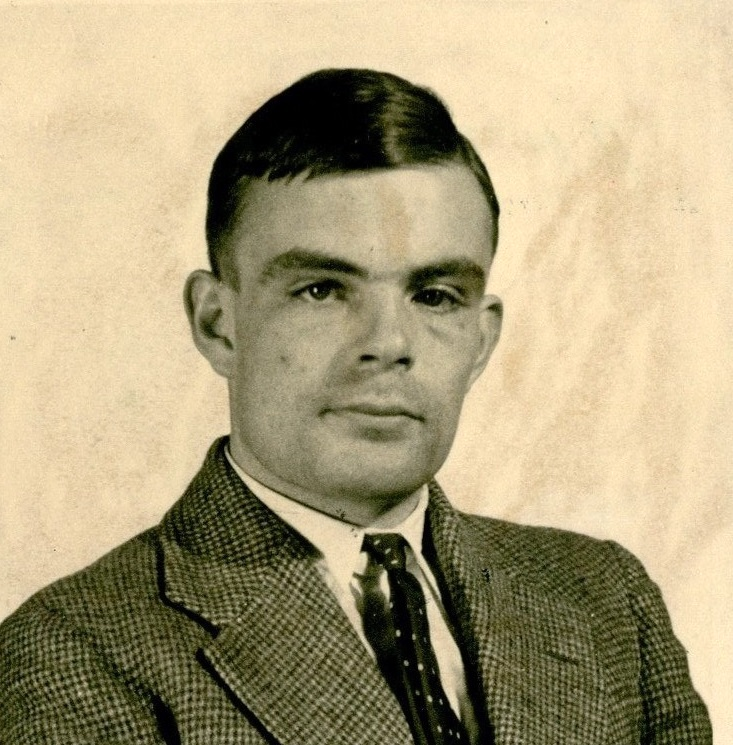
\includegraphics[width=3.5cm]{data/turing.jpeg}
				};
			}
			\visible<2>{
				\node[
					inner sep=0pt,
					draw=black,
					anchor=east
				] (patient) at (4.25, -1) {
					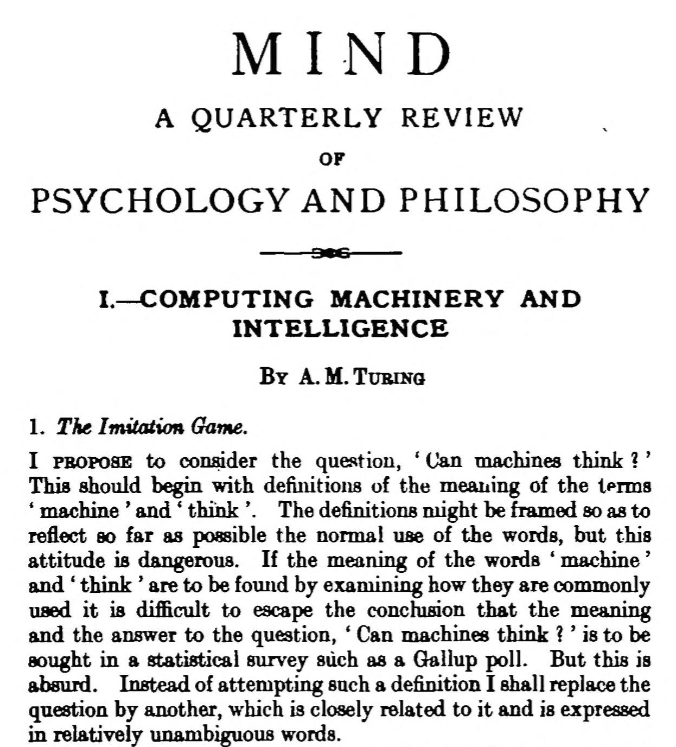
\includegraphics[width=4.5cm]{data/thinking.png}
				};
			}
			\visible<3->{
				\draw[very thick, gray] (-3.6, 2.75)  -- (-2.9, 2.75) {};
				\passivenode{-3.6}{Turing\\test\\(1950)}{0}
			}
			\visible<3>{
				\activenode{-2.9}{Dartmouth\\(1956)}{1}
			}
		\end{tikzpicture}
	\end{frame}

	\begin{frame}{The history of artificial intelligence} % Turing
		\begin{tikzpicture}
			\node[] at (0, 0) {};
			\node[] at (10.5, -7.5) {};

			\draw[very thick, gray] (0.5, -1)  -- (1.65, -1) {};

			\node[
				circle,
				draw=activehistory,
				fill=activehistory
			] at (1.65, -1) {};
			\node[
				anchor=north,
				activehistory,
				align=center,
				font=\small\linespread{0.9}\selectfont,
				text height=9pt,
				text depth=3pt,
				inner sep=0pt,
				align=center
			] at (1.65, -1.588) {Turing\\test\\(1950)};

			\node[inner sep=0pt, draw=black, label=below:{Alan Turing}] (patient) at (5.25, -4.25) {
				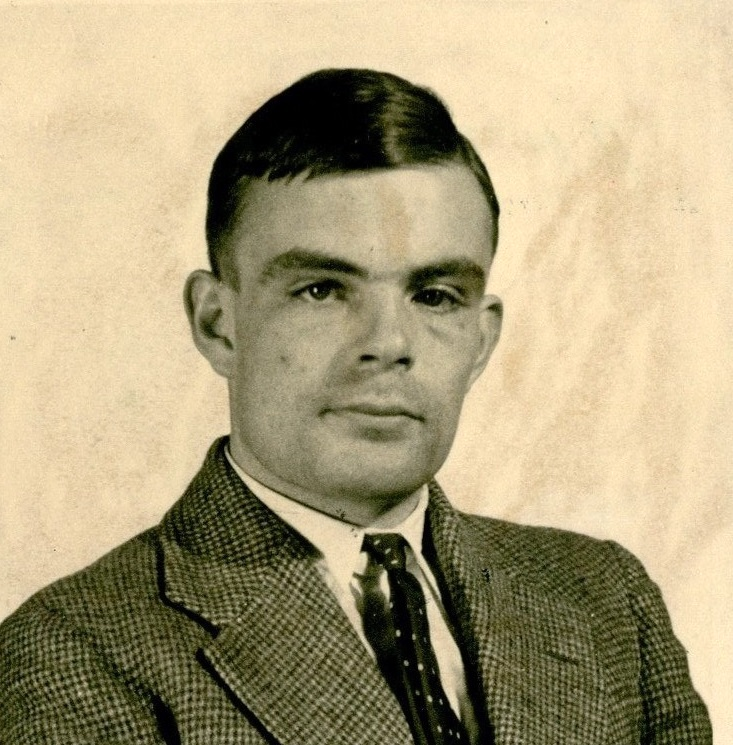
\includegraphics[width=4cm]{data/turing.jpeg}
			};
		\end{tikzpicture}
	\end{frame}

	\setbeamertemplate{footline}[turing]

	\begin{frame}{The history of artificial intelligence} % Turing test
		\begin{tikzpicture}
			\node[] at (0, 0) {};
			\node[] at (10.5, -7.5) {};

			\draw[very thick, gray] (0.5, -1)  -- (1.65, -1) {};

			\node[
				circle,
				draw=activehistory,
				fill=activehistory
			] at (1.65, -1) {};
			\node[
				anchor=north,
				activehistory,
				align=center,
				font=\small\linespread{0.9}\selectfont,
				text height=9pt,
				text depth=3pt,
				inner sep=0pt,
				align=center
			] at (1.65, -1.588) {Turing\\test\\(1950)};

			\node[inner sep=0pt, draw=black] (patient) at (5.25, -4.25) {
				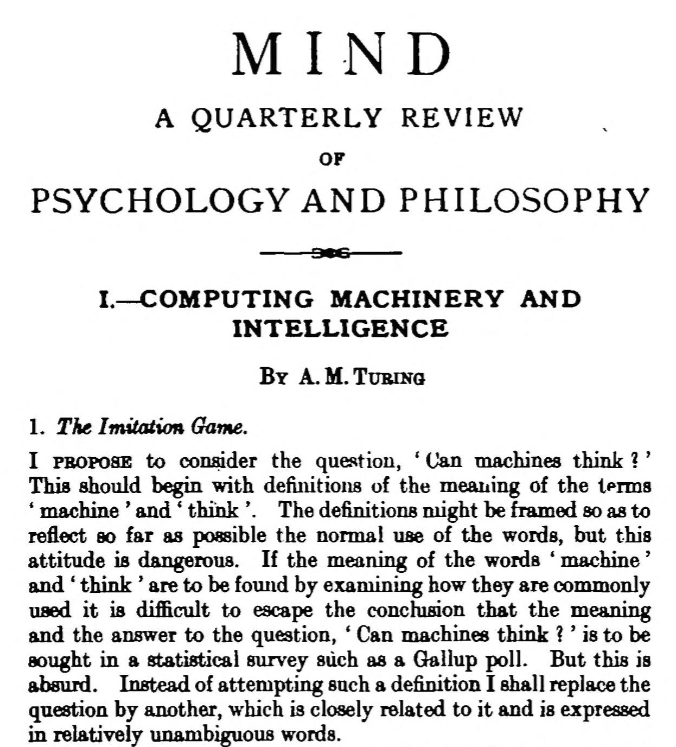
\includegraphics[width=5cm]{data/thinking.png}
			};
		\end{tikzpicture}
	\end{frame}

	\begin{frame}{The history of artificial intelligence} % Dartmouth
		\begin{tikzpicture}
			\node[] at (0, 0) {};
			\node[] at (10.5, -7.5) {};

			\draw[very thick, gray] (0.5, -1)  -- (2.35, -1) {};

			\node[
				circle,
				draw=passivehistory,
				fill=passivehistory
			] at (1.65, -1) {};
			\node[
				anchor=north,
				passivehistory,
				align=center,
				font=\small\linespread{0.9}\selectfont,
				text height=9pt,
				text depth=3pt,
				inner sep=0pt,
				align=center
			] at (1.65, -1.588) {Turing\\test\\(1950)};

			\node[
				circle,
				draw=activehistory,
				fill=activehistory,
			] at (2.35, -1) {};
			\node[
				anchor=south,
				activehistory,
				font=\small\linespread{0.9}\selectfont,
				text height=9pt,
				text depth=3pt,
				inner sep=0pt,
				align=center
			] at (2.35, -0.87) {Dartmouth\\(1956)};

			\node[inner sep=0pt] (patient) at (5.25, -4.75) {
				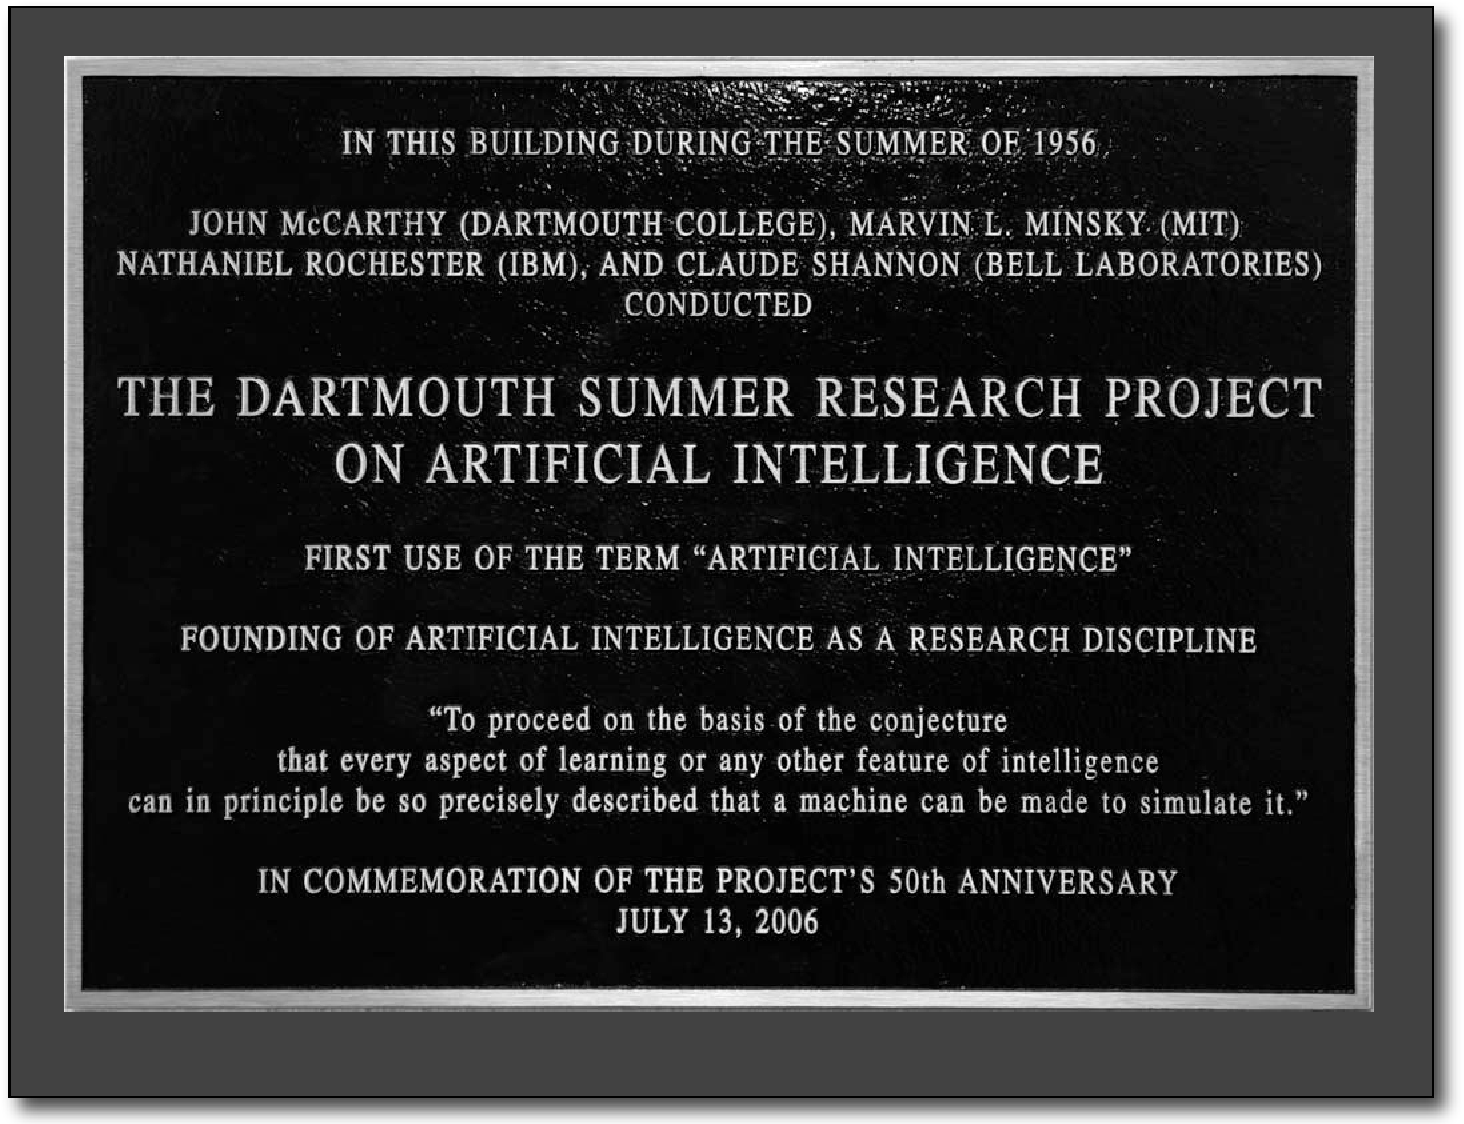
\includegraphics[width=6cm]{data/dartmouth.png}
			};
		\end{tikzpicture}
	\end{frame}

	\setbeamertemplate{footline}[neuron]

	\begin{frame}{The history of artificial intelligence} % Perceptron: Neuron
		\begin{tikzpicture}
			\node[] at (0, 0) {};
			\node[] at (10.5, -7.5) {};

			\draw[very thick, gray] (0.5, -1)  -- (2.68, -1) {};

			\node[
				circle,
				draw=passivehistory,
				fill=passivehistory
			] at (1.65, -1) {};
			\node[
				anchor=north,
				passivehistory,
				align=center,
				font=\small\linespread{0.9}\selectfont,
				text height=9pt,
				text depth=3pt,
				inner sep=0pt,
				align=center
			] at (1.65, -1.588) {Turing\\test\\(1950)};

			\node[
				circle,
				draw=passivehistory,
				fill=passivehistory,
			] at (2.35, -1) {};
			\node[
				anchor=south,
				passivehistory,
				font=\small\linespread{0.9}\selectfont,
				text height=9pt,
				text depth=3pt,
				inner sep=0pt,
				align=center
			] at (2.35, -0.87) {Dartmouth\\(1956)};

			\node[
				circle,
				draw=activehistory,
				fill=activehistory,
			] at (2.68, -1) {};
			\node[
				anchor=north,
				activehistory,
				font=\small\linespread{0.9}\selectfont,
				text height=9pt,
				text depth=3pt,
				inner sep=0pt,
				align=center
			] at (2.68, -1.375) {Perceptron\\(1958)};

			\node[draw=black, inner sep=5pt, fill=white] (patient) at (2.875, -4.75) {
				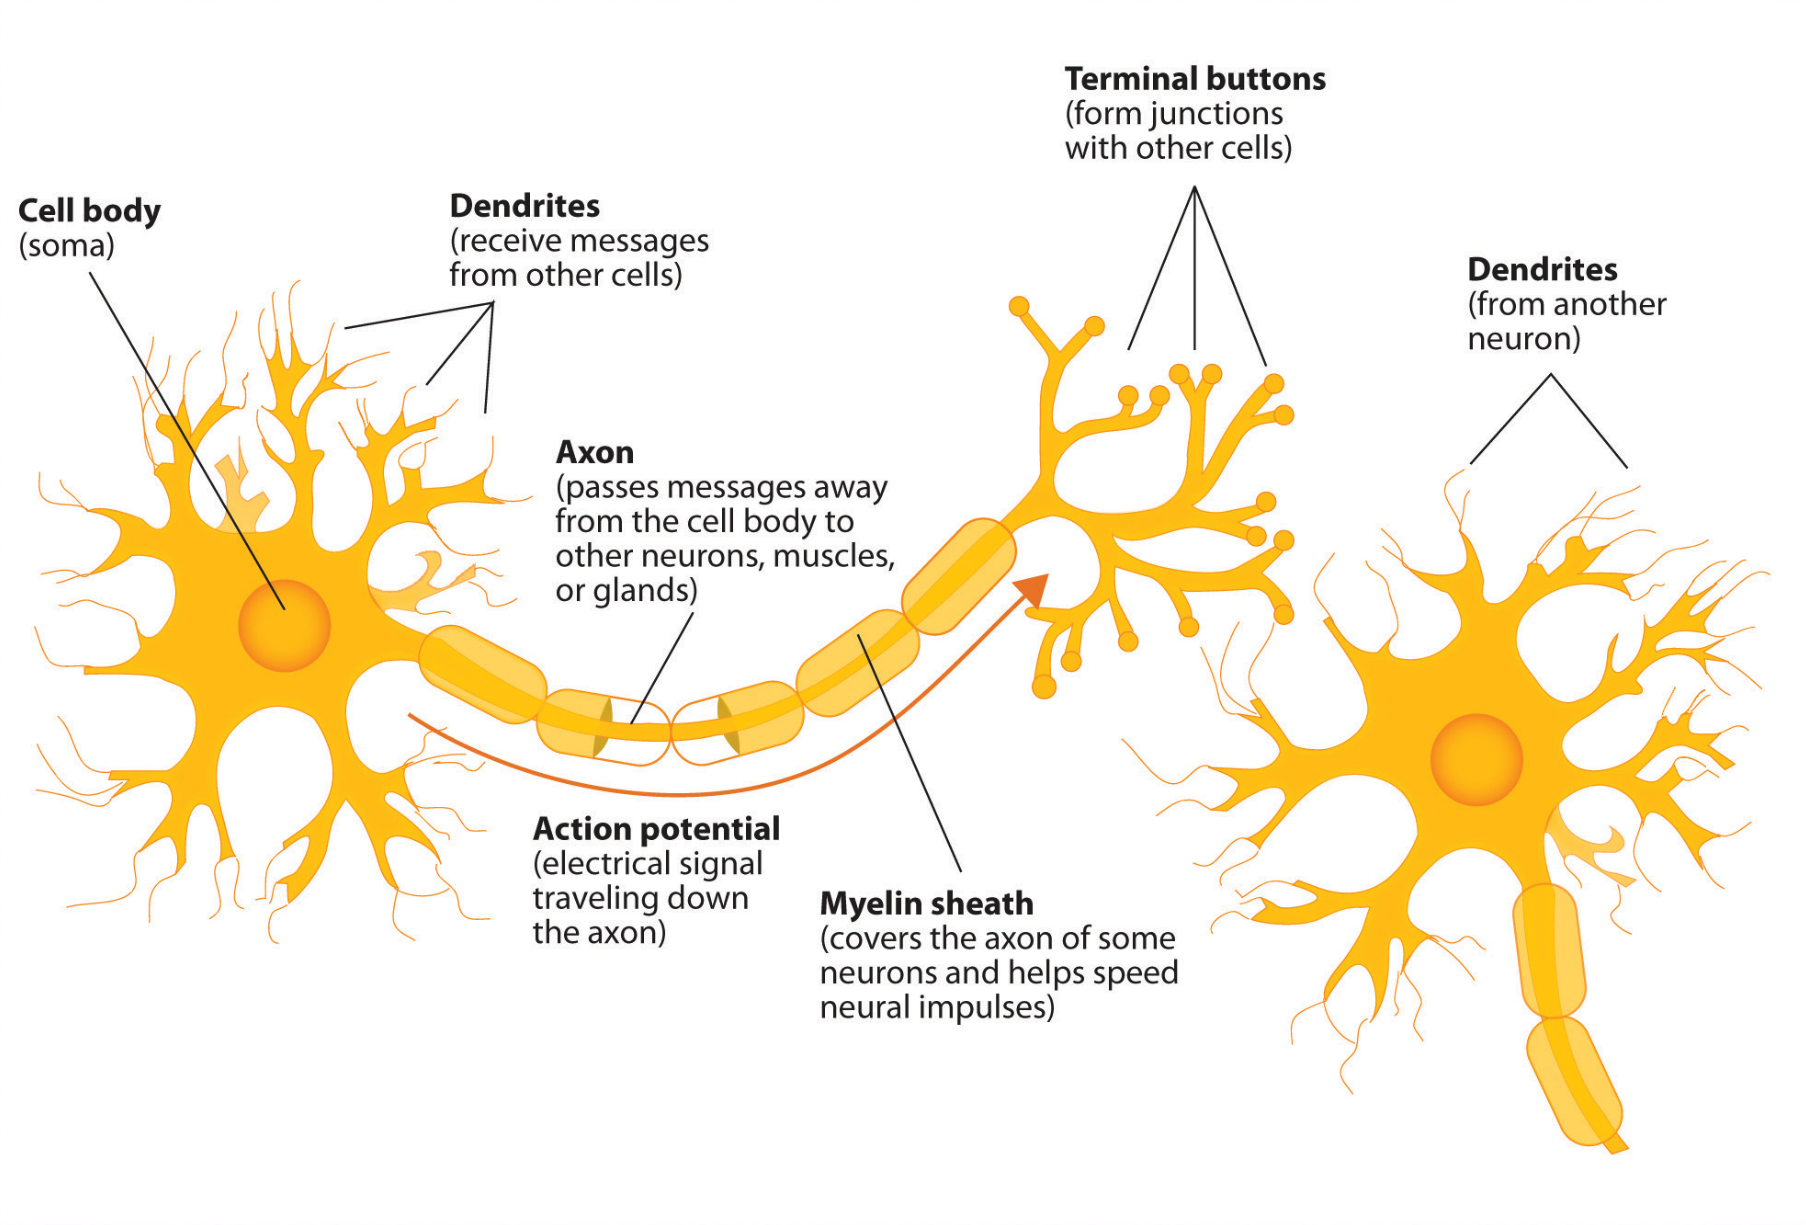
\includegraphics[width=4cm]{data/neuron.png}
			};
		\end{tikzpicture}
	\end{frame}

	\begin{frame}{The history of artificial intelligence} % Perceptron
		\begin{tikzpicture}
			\node[] at (0, 0) {};
			\node[] at (10.5, -7.5) {};

			\draw[very thick, gray] (0.5, -1)  -- (2.68, -1) {};

			\node[
				circle,
				draw=passivehistory,
				fill=passivehistory
			] at (1.65, -1) {};
			\node[
				anchor=north,
				passivehistory,
				align=center,
				font=\small\linespread{0.9}\selectfont,
				text height=9pt,
				text depth=3pt,
				inner sep=0pt,
				align=center
			] at (1.65, -1.588) {Turing\\test\\(1950)};

			\node[
				circle,
				draw=passivehistory,
				fill=passivehistory,
			] at (2.35, -1) {};
			\node[
				anchor=south,
				passivehistory,
				font=\small\linespread{0.9}\selectfont,
				text height=9pt,
				text depth=3pt,
				inner sep=0pt,
				align=center
			] at (2.35, -0.87) {Dartmouth\\(1956)};

			\node[
				circle,
				draw=activehistory,
				fill=activehistory,
			] at (2.68, -1) {};
			\node[
				anchor=north,
				activehistory,
				font=\small\linespread{0.9}\selectfont,
				text height=9pt,
				text depth=3pt,
				inner sep=0pt,
				align=center
			] at (2.68, -1.375) {Perceptron\\(1958)};

			\node[draw=black, inner sep=5pt, fill=white] (patient) at (2.875, -4.75) {
				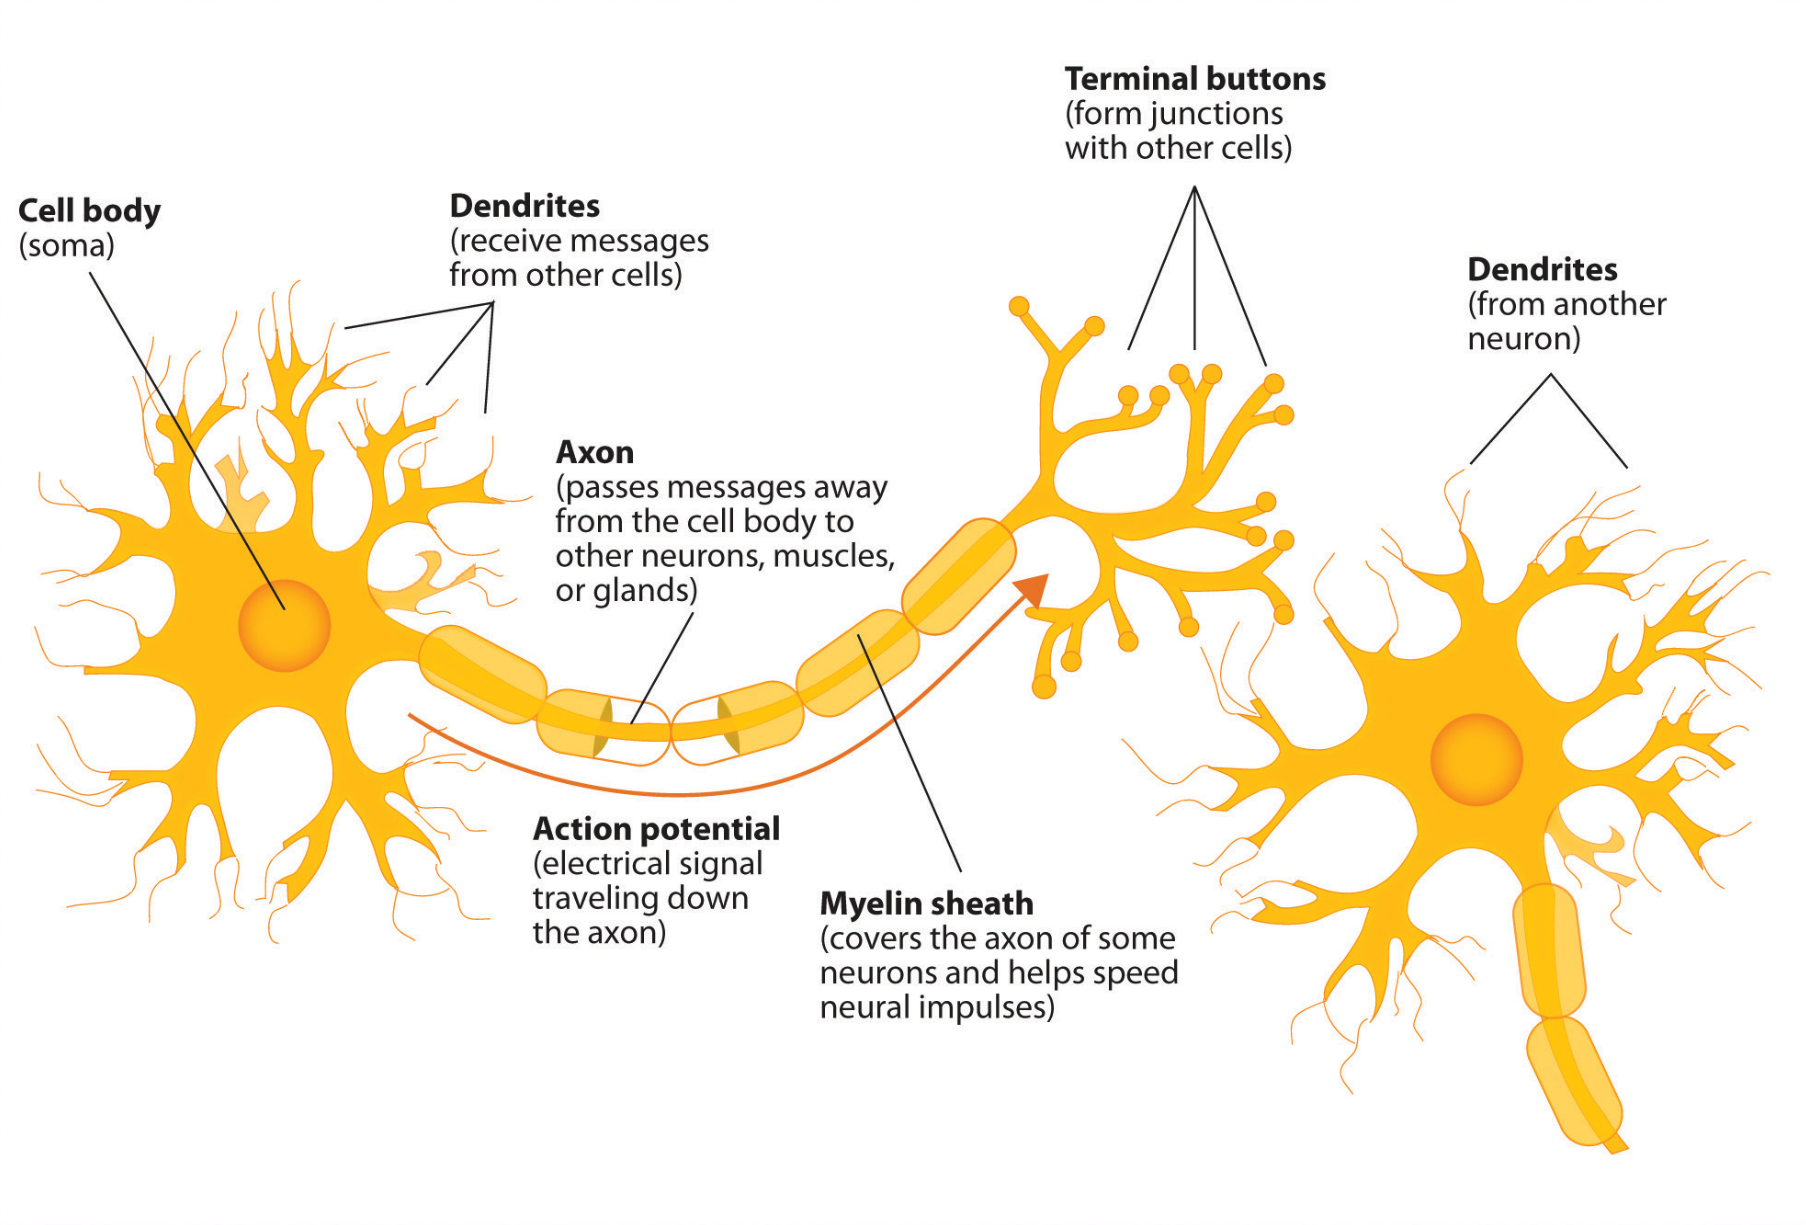
\includegraphics[width=4cm]{data/neuron.png}
			};

			\node[circle, draw=black, fill=nodefill, inner sep=2pt, text depth=0] (node) at (7.625, -4.75) {+};

			\node[] (x0) at (6.375, -3.75) {$\mathrm{input}_0$};
			\node[] (x1) at (6.375, -4.75) {$\mathrm{input}_1$};
			\node[] (x2) at (6.375, -5.75) {$\mathrm{input}_2$};

			\node[align=center] (out) at (8.875, -4.75) {$\mathrm{output}$\\$\mathrm{(0/1)}$};

			\draw[-Latex] (x0) -- (node) node [midway, above] {\small{$w_0$}};
			\draw[-Latex] (x1) -- (node) node [midway, below] {\small{$w_1$}};;
			\draw[-Latex] (x2) -- (node) node [midway, below] {\small{$w_2$}};;
			\draw[-Latex] (node) -- (out);
		\end{tikzpicture}
	\end{frame}

	\setbeamertemplate{footline}[eliza]

	\begin{frame}{The history of artificial intelligence} % Eliza
		\begin{tikzpicture}
			\node[] at (0, 0) {};
			\node[] at (10.5, -7.5) {};

			\draw[very thick, gray] (0.5, -1)  -- (3.28, -1) {};

			\node[
				circle,
				draw=passivehistory,
				fill=passivehistory
			] at (1.65, -1) {};
			\node[
				anchor=north,
				passivehistory,
				align=center,
				font=\small\linespread{0.9}\selectfont,
				text height=9pt,
				text depth=3pt,
				inner sep=0pt,
				align=center
			] at (1.65, -1.588) {Turing\\test\\(1950)};

			\node[
				circle,
				draw=passivehistory,
				fill=passivehistory,
			] at (2.35, -1) {};
			\node[
				anchor=south,
				passivehistory,
				font=\small\linespread{0.9}\selectfont,
				text height=9pt,
				text depth=3pt,
				inner sep=0pt,
				align=center
			] at (2.35, -0.87) {Dartmouth\\(1956)};

			\node[
				circle,
				draw=passivehistory,
				fill=passivehistory,
			] at (2.68, -1) {};
			\node[
				anchor=north,
				passivehistory,
				font=\small\linespread{0.9}\selectfont,
				text height=9pt,
				text depth=3pt,
				inner sep=0pt,
				align=center
			] at (2.68, -1.375) {Perceptron\\(1958)};

			\node[
				circle,
				draw=activehistory,
				fill=activehistory
			] at (3.28, -1) {};
			\node[
				anchor=south,
				activehistory,
				font=\small\linespread{0.9}\selectfont,
				text height=9pt,
				text depth=3pt,
				inner sep=0pt,
				align=center
			] at (3.28, -0.87) {Eliza\\(1964)};

			\node[draw=black, inner sep=5pt, fill=white] (patient) at (5.25, -4.75) {
				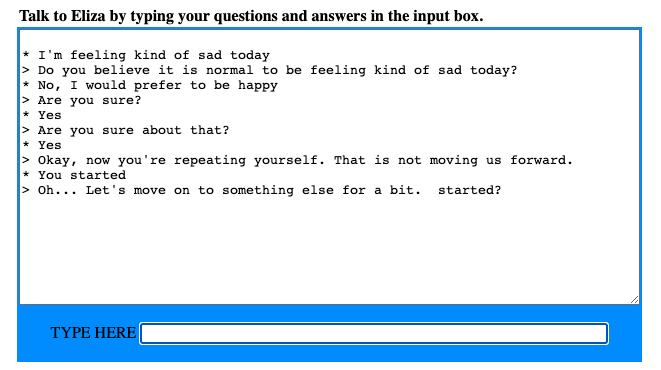
\includegraphics[width=7cm]{data/eliza.png}
			};
		\end{tikzpicture}
	\end{frame}

	\setbeamertemplate{footline}[mycin]

	\begin{frame}{The history of artificial intelligence} % Expert systems: Overview
		\begin{tikzpicture}
			\node[] at (0, 0) {};
			\node[] at (10.5, -7.5) {};

			\draw[very thick, gray] (0.5, -1)  -- (5.13, -1) {};

			\node[
				circle,
				draw=passivehistory,
				fill=passivehistory
			] at (1.65, -1) {};
			\node[
				anchor=north,
				passivehistory,
				align=center,
				font=\small\linespread{0.9}\selectfont,
				text height=9pt,
				text depth=3pt,
				inner sep=0pt,
				align=center
			] at (1.65, -1.588) {Turing\\test\\(1950)};

			\node[
				circle,
				draw=passivehistory,
				fill=passivehistory,
			] at (2.35, -1) {};
			\node[
				anchor=south,
				passivehistory,
				font=\small\linespread{0.9}\selectfont,
				text height=9pt,
				text depth=3pt,
				inner sep=0pt,
				align=center
			] at (2.35, -0.87) {Dartmouth\\(1956)};

			\node[
				circle,
				draw=passivehistory,
				fill=passivehistory,
			] at (2.68, -1) {};
			\node[
				anchor=north,
				passivehistory,
				font=\small\linespread{0.9}\selectfont,
				text height=9pt,
				text depth=3pt,
				inner sep=0pt,
				align=center
			] at (2.68, -1.375) {Perceptron\\(1958)};

			\node[
				circle,
				draw=passivehistory,
				fill=passivehistory
			] at (3.28, -1) {};
			\node[
				circle,
				draw=passivehistory,
				fill=passivehistory,
			] at (2.35, -1) {};
			\node[
				anchor=south,
				passivehistory,
				font=\small\linespread{0.9}\selectfont,
				text height=9pt,
				text depth=3pt,
				inner sep=0pt,
				align=center
			] at (3.28, -0.87) {Eliza\\(1964)};

			\node[
				circle,
				draw=activehistory,
				fill=activehistory
			] at (5.13, -1) {};
			\node[
				anchor=north,
				activehistory,
				font=\small\linespread{0.9}\selectfont,
				text height=9pt,
				text depth=3pt,
				inner sep=0pt,
				align=center
			] at (5.13, -1.625) {Expert\\systems\\(1980s)};

			\node[] (patient) at (5.25, -3.25) {
				\Huge{\emoji{face-with-medical-mask}}
			};
			\node[draw=black, align=center ] (interface) at ($ (patient.south) - (0, 0.8) $) {
				User interface
			};

			\node[draw=black] (inference) at ($ (interface.south) - (0, 0.5) $) {
				Inference engine
			};
			\node[draw=black] (database) at ($ (inference.south) - (0, 0.5) $) {
				Knowledge database
			};
			\node[] (doctor) at ($ (database.south) - (0, 0.9) $) {
				\Huge{\emoji{woman-scientist}}
			};

			\draw[-Latex] ($ (patient.south) - (0.1, 0) $) -- ($ (interface.north) - (0.1, 0) $);
			\draw[Latex-] ($ (patient.south) + (0.1, 0) $) -- ($ (interface.north) + (0.1, 0) $);
			\draw[-Latex] ($ (interface.south) - (0.1, 0) $) -- ($ (inference.north) - (0.1, 0) $);
			\draw[Latex-] ($ (interface.south) + (0.1, 0) $) -- ($ (inference.north) + (0.1, 0) $);
			\draw[Latex-] (inference.south) -- (database.north);
			\draw[Latex-, dashed] (database.south) -- (doctor.north);

			\draw[densely dotted] ($ (interface.north west) + (-1.3, 0.1) $) rectangle ($ (database.south east) + (1, -0.1) $);
			\node[anchor=south west] at ($ (interface.north west) + (-1.3, 0.1) $) {MYCIN};

			\node[anchor=north east] at ($ (patient.south) - (0.1, 0.05) $) {\small{Query}};
			\node[anchor=north west] at ($ (patient.south) - (-0.1, 0.05) $) {\small{Response}};
		\end{tikzpicture}
	\end{frame}

	\begin{frame}{The history of artificial intelligence} % Expert systems: Overview
		\begin{tikzpicture}
			\node[] at (0, 0) {};
			\node[] at (10.5, -7.5) {};

			\draw[very thick, gray] (0.5, -1)  -- (5.13, -1) {};

			\node[
				circle,
				draw=passivehistory,
				fill=passivehistory
			] at (1.65, -1) {};
			\node[
				anchor=north,
				passivehistory,
				align=center,
				font=\small\linespread{0.9}\selectfont,
				text height=9pt,
				text depth=3pt,
				inner sep=0pt,
				align=center
			] at (1.65, -1.588) {Turing\\test\\(1950)};

			\node[
				circle,
				draw=passivehistory,
				fill=passivehistory,
			] at (2.35, -1) {};
			\node[
				anchor=south,
				passivehistory,
				font=\small\linespread{0.9}\selectfont,
				text height=9pt,
				text depth=3pt,
				inner sep=0pt,
				align=center
			] at (2.35, -0.87) {Dartmouth\\(1956)};

			\node[
				circle,
				draw=passivehistory,
				fill=passivehistory,
			] at (2.68, -1) {};
			\node[
				anchor=north,
				passivehistory,
				font=\small\linespread{0.9}\selectfont,
				text height=9pt,
				text depth=3pt,
				inner sep=0pt,
				align=center
			] at (2.68, -1.375) {Perceptron\\(1958)};

			\node[
				circle,
				draw=passivehistory,
				fill=passivehistory
			] at (3.28, -1) {};
			\node[
				circle,
				draw=passivehistory,
				fill=passivehistory,
			] at (2.35, -1) {};
			\node[
				anchor=south,
				passivehistory,
				font=\small\linespread{0.9}\selectfont,
				text height=9pt,
				text depth=3pt,
				inner sep=0pt,
				align=center
			] at (3.28, -0.87) {Eliza\\(1964)};

			\node[
				circle,
				draw=activehistory,
				fill=activehistory
			] at (5.13, -1) {};
			\node[
				anchor=north,
				activehistory,
				font=\small\linespread{0.9}\selectfont,
				text height=9pt,
				text depth=3pt,
				inner sep=0pt,
				align=center
			] at (5.13, -1.625) {Expert\\systems\\(1980s)};

			\node[inner sep=0pt, draw=black] (patient) at (5.25, -4.75) {
				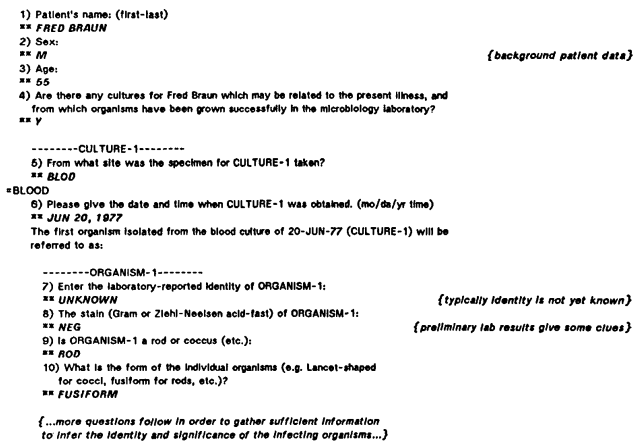
\includegraphics[width=7cm]{data/mycin.png}
			};
		\end{tikzpicture}
	\end{frame}

	\setbeamertemplate{footline}[backprop]

	\begin{frame}{The history of artificial intelligence} % ANNs: Paper
		\begin{tikzpicture}
			\node[] at (0, 0) {};
			\node[] at (10.5, -7.5) {};

			\draw[very thick, gray] (0.5, -1)  -- (5.82, -1) {};

			\node[
				circle,
				draw=passivehistory,
				fill=passivehistory
			] at (1.65, -1) {};
			\node[
				anchor=north,
				passivehistory,
				align=center,
				font=\small\linespread{0.9}\selectfont,
				text height=9pt,
				text depth=3pt,
				inner sep=0pt,
				align=center
			] at (1.65, -1.588) {Turing\\test\\(1950)};

			\node[
				circle,
				draw=passivehistory,
				fill=passivehistory,
			] at (2.35, -1) {};
			\node[
				anchor=south,
				passivehistory,
				font=\small\linespread{0.9}\selectfont,
				text height=9pt,
				text depth=3pt,
				inner sep=0pt,
				align=center
			] at (2.35, -0.87) {Dartmouth\\(1956)};

			\node[
				circle,
				draw=passivehistory,
				fill=passivehistory,
			] at (2.68, -1) {};
			\node[
				anchor=north,
				passivehistory,
				font=\small\linespread{0.9}\selectfont,
				text height=9pt,
				text depth=3pt,
				inner sep=0pt,
				align=center
			] at (2.68, -1.375) {Perceptron\\(1958)};

			\node[
				circle,
				draw=passivehistory,
				fill=passivehistory
			] at (3.28, -1) {};
			\node[
				circle,
				draw=passivehistory,
				fill=passivehistory,
			] at (2.35, -1) {};
			\node[
				anchor=south,
				passivehistory,
				font=\small\linespread{0.9}\selectfont,
				text height=9pt,
				text depth=3pt,
				inner sep=0pt,
				align=center
			] at (3.28, -0.87) {Eliza\\(1964)};

			\node[
				circle,
				draw=passivehistory,
				fill=passivehistory
			] at (5.13, -1) {};
			\node[
				anchor=north,
				passivehistory,
				font=\small\linespread{0.9}\selectfont,
				text height=9pt,
				text depth=3pt,
				inner sep=0pt,
				align=center
			] at (5.13, -1.625) {Expert\\systems\\(1980s)};

			\node[
				circle,
				draw=activehistory,
				fill=activehistory
			] at (5.82, -1) {};
			\node[
				anchor=south,
				activehistory,
				font=\small\linespread{0.9}\selectfont,
				text height=9pt,
				text depth=3pt,
				inner sep=0pt,
				align=center
			] at (5.82, -0.87) {ANNs\\(1986)};

			\node[inner sep=0pt, draw=black] (img3) at (5.25, -4.75) {
				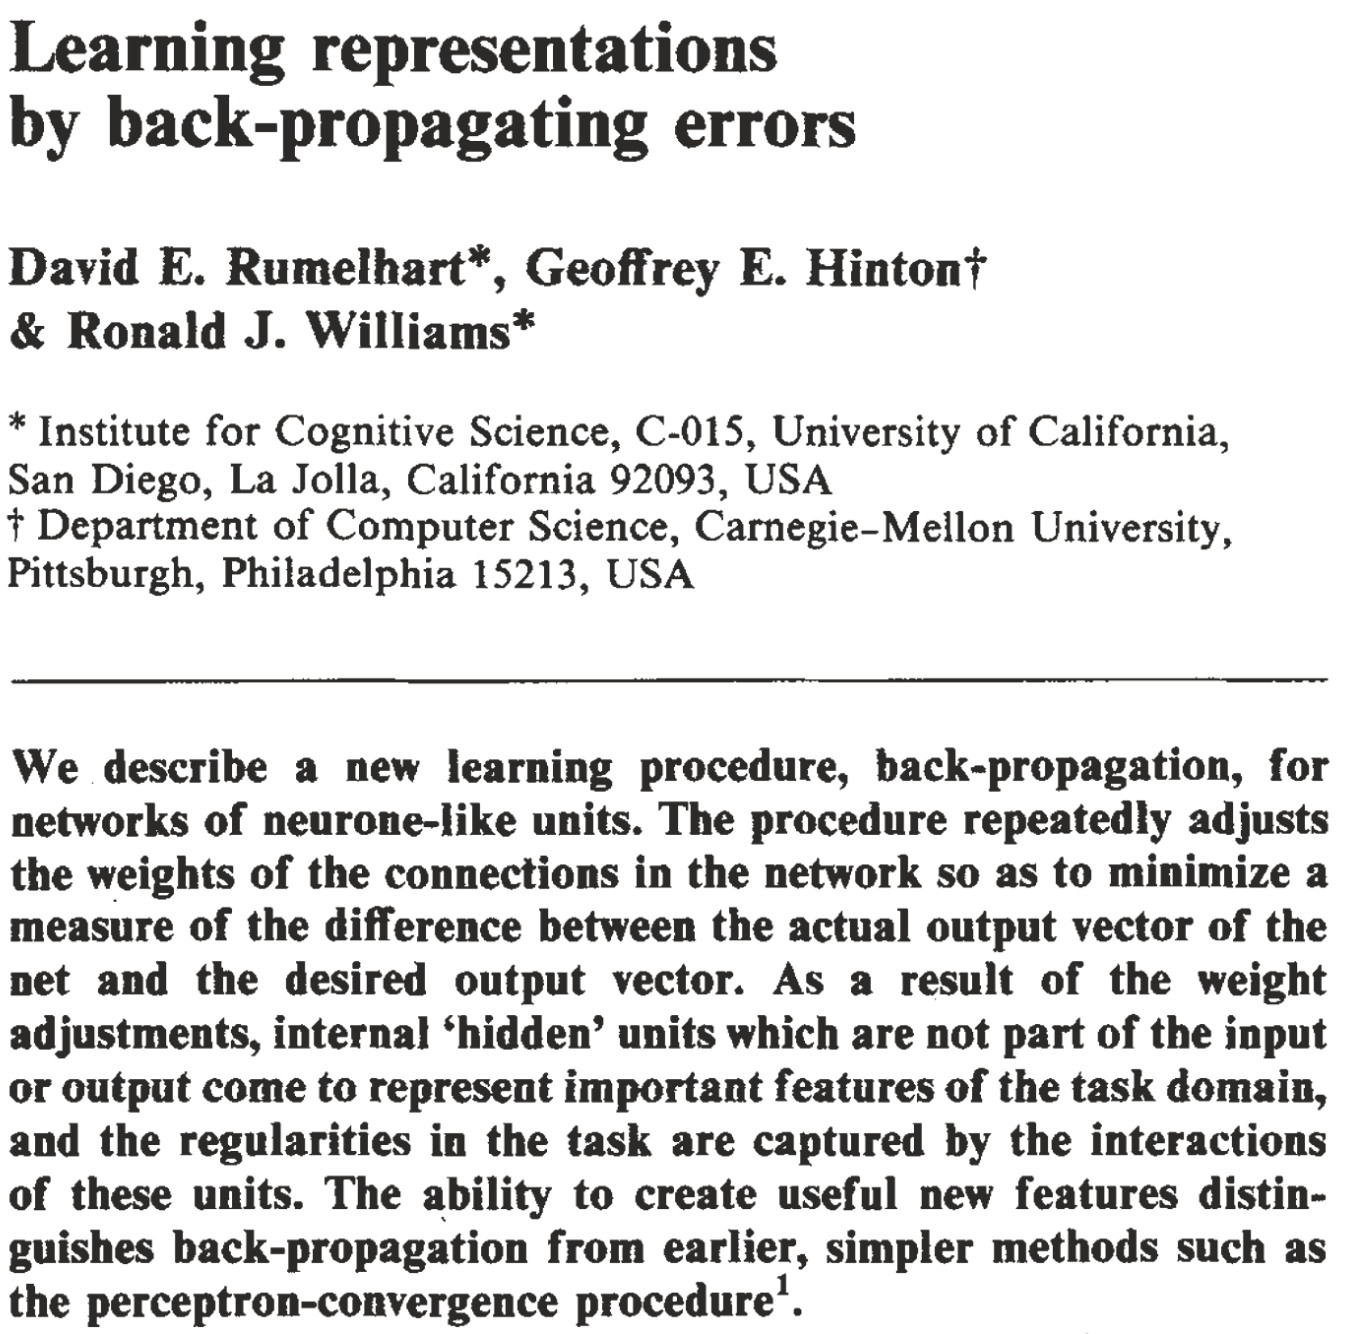
\includegraphics[width=4cm]{data/backprop.png}
			};
		\end{tikzpicture}
	\end{frame}

	\begin{frame}{The history of artificial intelligence} % ANNs: Perceptron
		\begin{tikzpicture}
			\node[] at (0, 0) {};
			\node[] at (10.5, -7.5) {};

			\draw[very thick, gray] (0.5, -1)  -- (5.82, -1) {};

			\node[
				circle,
				draw=passivehistory,
				fill=passivehistory
			] at (1.65, -1) {};
			\node[
				anchor=north,
				passivehistory,
				align=center,
				font=\small\linespread{0.9}\selectfont,
				text height=9pt,
				text depth=3pt,
				inner sep=0pt,
				align=center
			] at (1.65, -1.588) {Turing\\test\\(1950)};

			\node[
				circle,
				draw=passivehistory,
				fill=passivehistory,
			] at (2.35, -1) {};
			\node[
				anchor=south,
				passivehistory,
				font=\small\linespread{0.9}\selectfont,
				text height=9pt,
				text depth=3pt,
				inner sep=0pt,
				align=center
			] at (2.35, -0.87) {Dartmouth\\(1956)};

			\node[
				circle,
				draw=passivehistory,
				fill=passivehistory,
			] at (2.68, -1) {};
			\node[
				anchor=north,
				passivehistory,
				font=\small\linespread{0.9}\selectfont,
				text height=9pt,
				text depth=3pt,
				inner sep=0pt,
				align=center
			] at (2.68, -1.375) {Perceptron\\(1958)};

			\node[
				circle,
				draw=passivehistory,
				fill=passivehistory
			] at (3.28, -1) {};
			\node[
				circle,
				draw=passivehistory,
				fill=passivehistory,
			] at (2.35, -1) {};
			\node[
				anchor=south,
				passivehistory,
				font=\small\linespread{0.9}\selectfont,
				text height=9pt,
				text depth=3pt,
				inner sep=0pt,
				align=center
			] at (3.28, -0.87) {Eliza\\(1964)};

			\node[
				circle,
				draw=passivehistory,
				fill=passivehistory
			] at (5.13, -1) {};
			\node[
				anchor=north,
				passivehistory,
				font=\small\linespread{0.9}\selectfont,
				text height=9pt,
				text depth=3pt,
				inner sep=0pt,
				align=center
			] at (5.13, -1.625) {Expert\\systems\\(1980s)};

			\node[
				circle,
				draw=activehistory,
				fill=activehistory
			] at (5.82, -1) {};
			\node[
				anchor=south,
				activehistory,
				font=\small\linespread{0.9}\selectfont,
				text height=9pt,
				text depth=3pt,
				inner sep=0pt,
				align=center
			] at (5.82, -0.87) {ANNs\\(1986)};

			\node[inner sep=0pt, minimum size=0.4cm, draw=black, circle, fill=nodefill] (n00) at (5.25, -4.75) {};

			\node[] (x0) at (4, -4) {$\mathrm{input}_0$};
			\node[] (x1) at (4, -4.75) {$\mathrm{input}_1$};
			\node[] (x2) at (4, -5.5) {$\mathrm{input}_2$};

			\node[] (out) at (6.5, -4.75) {$\mathrm{output}$};

			\draw[-] (x0.east) -- (n00);
			\draw[-] (x1.east) -- (n00);
			\draw[-] (x2.east) -- (n00);

			\draw[->] (n00) -- (out);
		\end{tikzpicture}
	\end{frame}

	\begin{frame}{The history of artificial intelligence} % ANNs: Neural net
		\begin{tikzpicture}
			\node[] at (0, 0) {};
			\node[] at (10.5, -7.5) {};

			\draw[very thick, gray] (0.5, -1)  -- (5.82, -1) {};

			\node[
				circle,
				draw=passivehistory,
				fill=passivehistory
			] at (1.65, -1) {};
			\node[
				anchor=north,
				passivehistory,
				align=center,
				font=\small\linespread{0.9}\selectfont,
				text height=9pt,
				text depth=3pt,
				inner sep=0pt,
				align=center
			] at (1.65, -1.588) {Turing\\test\\(1950)};

			\node[
				circle,
				draw=passivehistory,
				fill=passivehistory,
			] at (2.35, -1) {};
			\node[
				anchor=south,
				passivehistory,
				font=\small\linespread{0.9}\selectfont,
				text height=9pt,
				text depth=3pt,
				inner sep=0pt,
				align=center
			] at (2.35, -0.87) {Dartmouth\\(1956)};

			\node[
				circle,
				draw=passivehistory,
				fill=passivehistory,
			] at (2.68, -1) {};
			\node[
				anchor=north,
				passivehistory,
				font=\small\linespread{0.9}\selectfont,
				text height=9pt,
				text depth=3pt,
				inner sep=0pt,
				align=center
			] at (2.68, -1.375) {Perceptron\\(1958)};

			\node[
				circle,
				draw=passivehistory,
				fill=passivehistory
			] at (3.28, -1) {};
			\node[
				circle,
				draw=passivehistory,
				fill=passivehistory,
			] at (2.35, -1) {};
			\node[
				anchor=south,
				passivehistory,
				font=\small\linespread{0.9}\selectfont,
				text height=9pt,
				text depth=3pt,
				inner sep=0pt,
				align=center
			] at (3.28, -0.87) {Eliza\\(1964)};

			\node[
				circle,
				draw=passivehistory,
				fill=passivehistory
			] at (5.13, -1) {};
			\node[
				anchor=north,
				passivehistory,
				font=\small\linespread{0.9}\selectfont,
				text height=9pt,
				text depth=3pt,
				inner sep=0pt,
				align=center
			] at (5.13, -1.625) {Expert\\systems\\(1980s)};

			\node[
				circle,
				draw=activehistory,
				fill=activehistory
			] at (5.82, -1) {};
			\node[
				anchor=south,
				activehistory,
				font=\small\linespread{0.9}\selectfont,
				text height=9pt,
				text depth=3pt,
				inner sep=0pt,
				align=center
			] at (5.82, -0.87) {ANNs\\(1986)};

			\node[] (x0) at (2.5, -4) {$\mathrm{input}_0$};
			\node[] (x1) at (2.5, -4.75) {$\mathrm{input}_1$};
			\node[] (x2) at (2.5, -5.5) {$\mathrm{input}_2$};

			\node[inner sep=0pt, minimum size=0.4cm, draw=black, circle, fill=nodefill] (n00) at (3.75, -3.75) {};
			\node[inner sep=0pt, minimum size=0.4cm, draw=black, circle, fill=nodefill] (n01) at (3.75, -4.25) {};
			\node[inner sep=0pt, minimum size=0.4cm, draw=black, circle, fill=nodefill] (n02) at (3.75, -4.75) {};
			\node[inner sep=0pt, minimum size=0.4cm, draw=black, circle, fill=nodefill] (n03) at (3.75, -5.25) {};
			\node[inner sep=0pt, minimum size=0.4cm, draw=black, circle, fill=nodefill] (n04) at (3.75, -5.75) {};

			\node[inner sep=0pt, minimum size=0.4cm, draw=black, circle, fill=nodefill] (n10) at (4.5, -4) {};
			\node[inner sep=0pt, minimum size=0.4cm, draw=black, circle, fill=nodefill] (n11) at (4.5, -4.5) {};
			\node[inner sep=0pt, minimum size=0.4cm, draw=black, circle, fill=nodefill] (n12) at (4.5, -5) {};
			\node[inner sep=0pt, minimum size=0.4cm, draw=black, circle, fill=nodefill] (n13) at (4.5, -5.5) {};

			\node[inner sep=0pt, minimum size=0.4cm, draw=black, circle, fill=nodefill] (n20) at (5.25, -4.25) {};
			\node[inner sep=0pt, minimum size=0.4cm, draw=black, circle, fill=nodefill] (n21) at (5.25, -4.75) {};
			\node[inner sep=0pt, minimum size=0.4cm, draw=black, circle, fill=nodefill] (n22) at (5.25, -5.25) {};

			\node[inner sep=0pt, minimum size=0.4cm, draw=black, circle, fill=nodefill] (n30) at (6, -4.5) {};
			\node[inner sep=0pt, minimum size=0.4cm, draw=black, circle, fill=nodefill] (n31) at (6, -5) {};

			\node[inner sep=0pt, minimum size=0.4cm, draw=black, circle, fill=nodefill, text depth=0] (n40) at (6.75, -4.75) {};
			\node[] (out) at (8, -4.75) {$\mathrm{output}$};

			\draw[-] (x0.east) -- (n00);
			\draw[-] (x0.east) -- (n01);
			\draw[-] (x0.east) -- (n02);
			\draw[-] (x0.east) -- (n03);
			\draw[-] (x0.east) -- (n04);
			\draw[-] (x1.east) -- (n00);
			\draw[-] (x1.east) -- (n01);
			\draw[-] (x1.east) -- (n02);
			\draw[-] (x1.east) -- (n03);
			\draw[-] (x1.east) -- (n04);
			\draw[-] (x2.east) -- (n00);
			\draw[-] (x2.east) -- (n01);
			\draw[-] (x2.east) -- (n02);
			\draw[-] (x2.east) -- (n03);
			\draw[-] (x2.east) -- (n04);

			\draw[-] (n00) -- (n10);
			\draw[-] (n00) -- (n11);
			\draw[-] (n00) -- (n12);
			\draw[-] (n00) -- (n13);
			\draw[-] (n01) -- (n10);
			\draw[-] (n01) -- (n11);
			\draw[-] (n01) -- (n12);
			\draw[-] (n01) -- (n13);
			\draw[-] (n02) -- (n10);
			\draw[-] (n02) -- (n11);
			\draw[-] (n02) -- (n12);
			\draw[-] (n02) -- (n13);
			\draw[-] (n03) -- (n10);
			\draw[-] (n03) -- (n11);
			\draw[-] (n03) -- (n12);
			\draw[-] (n03) -- (n13);
			\draw[-] (n04) -- (n10);
			\draw[-] (n04) -- (n11);
			\draw[-] (n04) -- (n12);
			\draw[-] (n04) -- (n13);

			\draw[-] (n10) -- (n20);
			\draw[-] (n10) -- (n21);
			\draw[-] (n10) -- (n22);
			\draw[-] (n11) -- (n20);
			\draw[-] (n11) -- (n21);
			\draw[-] (n11) -- (n22);
			\draw[-] (n12) -- (n20);
			\draw[-] (n12) -- (n21);
			\draw[-] (n12) -- (n22);
			\draw[-] (n13) -- (n20);
			\draw[-] (n13) -- (n21);
			\draw[-] (n13) -- (n22);

			\draw[-] (n20) -- (n30);
			\draw[-] (n20) -- (n31);
			\draw[-] (n21) -- (n30);
			\draw[-] (n21) -- (n31);
			\draw[-] (n22) -- (n30);
			\draw[-] (n22) -- (n31);

			\draw[-] (n30) -- (n40);
			\draw[-] (n31) -- (n40);

			\draw[->] (n40) -- (out);
		\end{tikzpicture}
	\end{frame}

	\begin{frame}{The history of artificial intelligence} % ANNs: Backprop
		\begin{tikzpicture}
			\node[] at (0, 0) {};
			\node[] at (10.5, -7.5) {};

			\draw[very thick, gray] (0.5, -1)  -- (5.82, -1) {};

			\node[
				circle,
				draw=passivehistory,
				fill=passivehistory
			] at (1.65, -1) {};
			\node[
				anchor=north,
				passivehistory,
				align=center,
				font=\small\linespread{0.9}\selectfont,
				text height=9pt,
				text depth=3pt,
				inner sep=0pt,
				align=center
			] at (1.65, -1.588) {Turing\\test\\(1950)};

			\node[
				circle,
				draw=passivehistory,
				fill=passivehistory,
			] at (2.35, -1) {};
			\node[
				anchor=south,
				passivehistory,
				font=\small\linespread{0.9}\selectfont,
				text height=9pt,
				text depth=3pt,
				inner sep=0pt,
				align=center
			] at (2.35, -0.87) {Dartmouth\\(1956)};

			\node[
				circle,
				draw=passivehistory,
				fill=passivehistory,
			] at (2.68, -1) {};
			\node[
				anchor=north,
				passivehistory,
				font=\small\linespread{0.9}\selectfont,
				text height=9pt,
				text depth=3pt,
				inner sep=0pt,
				align=center
			] at (2.68, -1.375) {Perceptron\\(1958)};

			\node[
				circle,
				draw=passivehistory,
				fill=passivehistory
			] at (3.28, -1) {};
			\node[
				circle,
				draw=passivehistory,
				fill=passivehistory,
			] at (2.35, -1) {};
			\node[
				anchor=south,
				passivehistory,
				font=\small\linespread{0.9}\selectfont,
				text height=9pt,
				text depth=3pt,
				inner sep=0pt,
				align=center
			] at (3.28, -0.87) {Eliza\\(1964)};

			\node[
				circle,
				draw=passivehistory,
				fill=passivehistory
			] at (5.13, -1) {};
			\node[
				anchor=north,
				passivehistory,
				font=\small\linespread{0.9}\selectfont,
				text height=9pt,
				text depth=3pt,
				inner sep=0pt,
				align=center
			] at (5.13, -1.625) {Expert\\systems\\(1980s)};

			\node[
				circle,
				draw=activehistory,
				fill=activehistory
			] at (5.82, -1) {};
			\node[
				anchor=south,
				activehistory,
				font=\small\linespread{0.9}\selectfont,
				text height=9pt,
				text depth=3pt,
				inner sep=0pt,
				align=center
			] at (5.82, -0.87) {ANNs\\(1986)};

			\node[] (x0) at (2.5, -4) {$\mathrm{input}_0$};
			\node[] (x1) at (2.5, -4.75) {$\mathrm{input}_1$};
			\node[] (x2) at (2.5, -5.5) {$\mathrm{input}_2$};

			\node[inner sep=0pt, minimum size=0.4cm, draw=black, circle, fill=nodefill] (n00) at (3.75, -3.75) {};
			\node[inner sep=0pt, minimum size=0.4cm, draw=black, circle, fill=nodefill] (n01) at (3.75, -4.25) {};
			\node[inner sep=0pt, minimum size=0.4cm, draw=black, circle, fill=nodefill] (n02) at (3.75, -4.75) {};
			\node[inner sep=0pt, minimum size=0.4cm, draw=black, circle, fill=nodefill] (n03) at (3.75, -5.25) {};
			\node[inner sep=0pt, minimum size=0.4cm, draw=black, circle, fill=nodefill] (n04) at (3.75, -5.75) {};

			\node[inner sep=0pt, minimum size=0.4cm, draw=black, circle, fill=nodefill] (n10) at (4.5, -4) {};
			\node[inner sep=0pt, minimum size=0.4cm, draw=black, circle, fill=nodefill] (n11) at (4.5, -4.5) {};
			\node[inner sep=0pt, minimum size=0.4cm, draw=black, circle, fill=nodefill] (n12) at (4.5, -5) {};
			\node[inner sep=0pt, minimum size=0.4cm, draw=black, circle, fill=nodefill] (n13) at (4.5, -5.5) {};

			\node[inner sep=0pt, minimum size=0.4cm, draw=black, circle, fill=nodefill] (n20) at (5.25, -4.25) {};
			\node[inner sep=0pt, minimum size=0.4cm, draw=black, circle, fill=nodefill] (n21) at (5.25, -4.75) {};
			\node[inner sep=0pt, minimum size=0.4cm, draw=black, circle, fill=nodefill] (n22) at (5.25, -5.25) {};

			\node[inner sep=0pt, minimum size=0.4cm, draw=black, circle, fill=nodefill] (n30) at (6, -4.5) {};
			\node[inner sep=0pt, minimum size=0.4cm, draw=black, circle, fill=nodefill] (n31) at (6, -5) {};

			\node[inner sep=0pt, minimum size=0.4cm, draw=black, circle, fill=nodefill, text depth=0] (n40) at (6.75, -4.75) {};
			\node[] (out) at (8, -4.75) {$\mathrm{output}$};

			\draw[-] (x0.east) -- (n00);
			\draw[-] (x0.east) -- (n01);
			\draw[-] (x0.east) -- (n02);
			\draw[-] (x0.east) -- (n03);
			\draw[-] (x0.east) -- (n04);
			\draw[-] (x1.east) -- (n00);
			\draw[-] (x1.east) -- (n01);
			\draw[-] (x1.east) -- (n02);
			\draw[-] (x1.east) -- (n03);
			\draw[-] (x1.east) -- (n04);
			\draw[-] (x2.east) -- (n00);
			\draw[-] (x2.east) -- (n01);
			\draw[-] (x2.east) -- (n02);
			\draw[-] (x2.east) -- (n03);
			\draw[-] (x2.east) -- (n04);

			\draw[Latex-, red] (n00) -- (n10);
			\draw[Latex-, red] (n00) -- (n11);
			\draw[Latex-, red] (n00) -- (n12);
			\draw[Latex-, red] (n00) -- (n13);
			\draw[Latex-, red] (n01) -- (n10);
			\draw[Latex-, red] (n01) -- (n11);
			\draw[Latex-, red] (n01) -- (n12);
			\draw[Latex-, red] (n01) -- (n13);
			\draw[Latex-, red] (n02) -- (n10);
			\draw[Latex-, red] (n02) -- (n11);
			\draw[Latex-, red] (n02) -- (n12);
			\draw[Latex-, red] (n02) -- (n13);
			\draw[Latex-, red] (n03) -- (n10);
			\draw[Latex-, red] (n03) -- (n11);
			\draw[Latex-, red] (n03) -- (n12);
			\draw[Latex-, red] (n03) -- (n13);
			\draw[Latex-, red] (n04) -- (n10);
			\draw[Latex-, red] (n04) -- (n11);
			\draw[Latex-, red] (n04) -- (n12);
			\draw[Latex-, red] (n04) -- (n13);

			\draw[Latex-, red] (n10) -- (n20);
			\draw[Latex-, red] (n10) -- (n21);
			\draw[Latex-, red] (n10) -- (n22);
			\draw[Latex-, red] (n11) -- (n20);
			\draw[Latex-, red] (n11) -- (n21);
			\draw[Latex-, red] (n11) -- (n22);
			\draw[Latex-, red] (n12) -- (n20);
			\draw[Latex-, red] (n12) -- (n21);
			\draw[Latex-, red] (n12) -- (n22);
			\draw[Latex-, red] (n13) -- (n20);
			\draw[Latex-, red] (n13) -- (n21);
			\draw[Latex-, red] (n13) -- (n22);

			\draw[Latex-, red] (n20) -- (n30);
			\draw[Latex-, red] (n20) -- (n31);
			\draw[Latex-, red] (n21) -- (n30);
			\draw[Latex-, red] (n21) -- (n31);
			\draw[Latex-, red] (n22) -- (n30);
			\draw[Latex-, red] (n22) -- (n31);

			\draw[Latex-, red] (n30) -- (n40);
			\draw[Latex-, red] (n31) -- (n40);

			\draw[Latex-, red] (n40) -- (out);
		\end{tikzpicture}
	\end{frame}

	\setbeamertemplate{footline}[default]

	\begin{frame}{The history of artificial intelligence} % Deep blue
		\begin{tikzpicture}
			\node[] at (0, 0) {};
			\node[] at (10.5, -7.5) {};

			\draw[very thick, gray] (0.5, -1)  -- (7.1, -1) {};

			\node[
				circle,
				draw=passivehistory,
				fill=passivehistory
			] at (1.65, -1) {};
			\node[
				anchor=north,
				passivehistory,
				align=center,
				font=\small\linespread{0.9}\selectfont,
				text height=9pt,
				text depth=3pt,
				inner sep=0pt,
				align=center
			] at (1.65, -1.588) {Turing\\test\\(1950)};

			\node[
				circle,
				draw=passivehistory,
				fill=passivehistory,
			] at (2.35, -1) {};
			\node[
				anchor=south,
				passivehistory,
				font=\small\linespread{0.9}\selectfont,
				text height=9pt,
				text depth=3pt,
				inner sep=0pt,
				align=center
			] at (2.35, -0.87) {Dartmouth\\(1956)};

			\node[
				circle,
				draw=passivehistory,
				fill=passivehistory,
			] at (2.68, -1) {};
			\node[
				anchor=north,
				passivehistory,
				font=\small\linespread{0.9}\selectfont,
				text height=9pt,
				text depth=3pt,
				inner sep=0pt,
				align=center
			] at (2.68, -1.375) {Perceptron\\(1958)};

			\node[
				circle,
				draw=passivehistory,
				fill=passivehistory
			] at (3.28, -1) {};
			\node[
				circle,
				draw=passivehistory,
				fill=passivehistory,
			] at (2.35, -1) {};
			\node[
				anchor=south,
				passivehistory,
				font=\small\linespread{0.9}\selectfont,
				text height=9pt,
				text depth=3pt,
				inner sep=0pt,
				align=center
			] at (3.28, -0.87) {Eliza\\(1964)};

			\node[
				circle,
				draw=passivehistory,
				fill=passivehistory
			] at (5.13, -1) {};
			\node[
				anchor=north,
				passivehistory,
				font=\small\linespread{0.9}\selectfont,
				text height=9pt,
				text depth=3pt,
				inner sep=0pt,
				align=center
			] at (5.13, -1.625) {Expert\\systems\\(1980s)};

			\node[
				circle,
				draw=passivehistory,
				fill=passivehistory
			] at (5.82, -1) {};
			\node[
				anchor=south,
				passivehistory,
				font=\small\linespread{0.9}\selectfont,
				text height=9pt,
				text depth=3pt,
				inner sep=0pt,
				align=center
			] at (5.82, -0.87) {ANNs\\(1986)};

			\node[
				circle,
				draw=activehistory,
				fill=activehistory
			] at (7.10, -1) {};
			\node[
				anchor=north,
				activehistory,
				font=\small\linespread{0.9}\selectfont,
				text height=9pt,
				text depth=3pt,
				inner sep=0pt,
				align=center
			] at (7.10, -1.372) {Deep blue\\(1997)};

			\node[inner sep=0pt, draw=black, label=below:{\small{DALL-E: "A robot playing chess"}}] (img) at (2.75, -4.75) {
				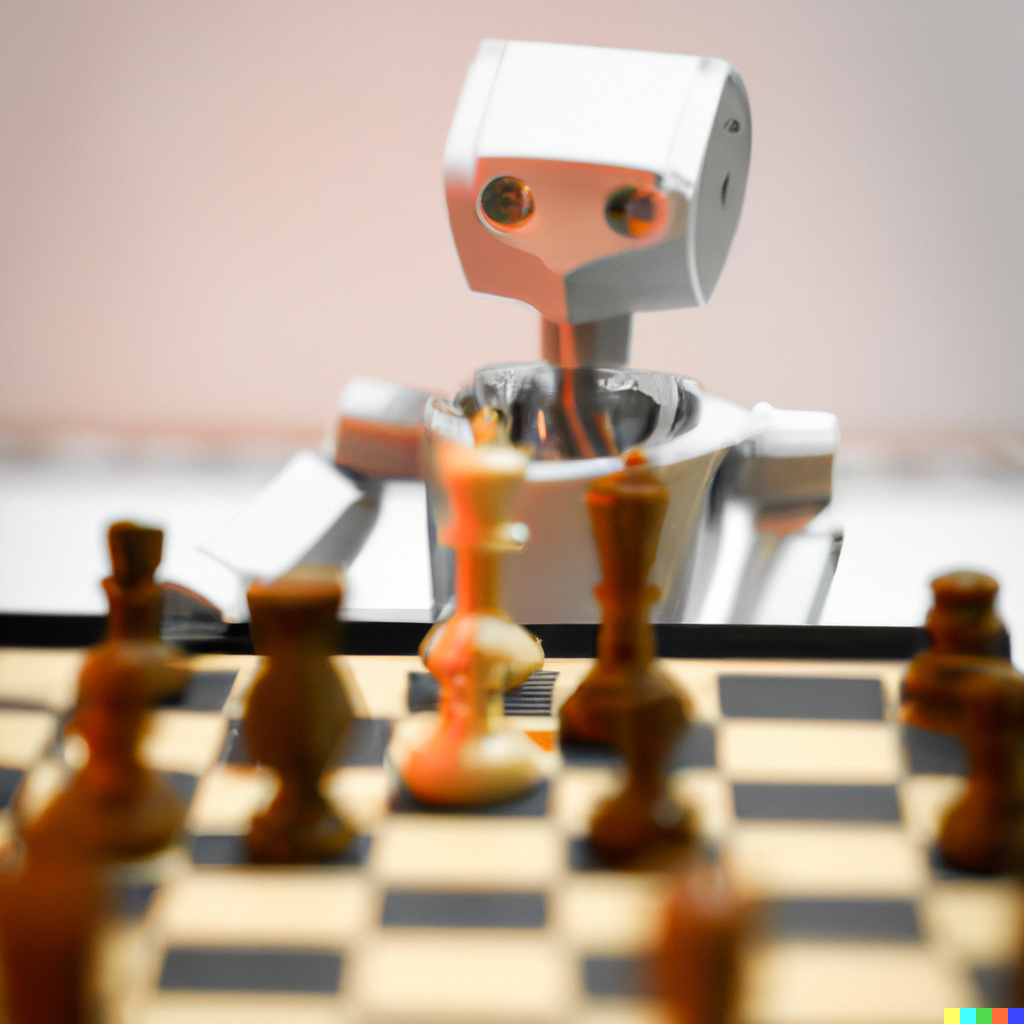
\includegraphics[width=4cm]{data/chess.png}
			};
			\node[anchor=north west, align=left] at ($ (img.north east)  + (0.1, 0) $) {
				\bullet\hspace{0.1cm}IBMs Deep Blue became the first computer\\ to beat the reigning human world champion\\ in chess.\\
				\bullet\hspace{0.1cm}Deep blue won with 3\textonehalf { }points to Garry\\Kasparovs 2\textonehalf{ } after six matches.\\
				\bullet\hspace{0.1cm}Kasparov famously stated that\\"Deep Blue was intelligent the way your\\programmable alarm clock is intelligent."\\
				\bullet\hspace{0.1cm}Combination of machine learning and\\preprogrammed knowledge from experts.
			};
		\end{tikzpicture}
	\end{frame}

	\begin{frame}{The history of artificial intelligence} %DL (image classification)
		\begin{tikzpicture}
			\node[] at (0, 0) {};
			\node[] at (10.5, -7.5) {};

			\draw[very thick, gray] (0.5, -1)  -- (8.84, -1) {};

			\node[
				circle,
				draw=passivehistory,
				fill=passivehistory
			] at (1.65, -1) {};
			\node[
				anchor=north,
				passivehistory,
				align=center,
				font=\small\linespread{0.9}\selectfont,
				text height=9pt,
				text depth=3pt,
				inner sep=0pt,
				align=center
			] at (1.65, -1.588) {Turing\\test\\(1950)};

			\node[
				circle,
				draw=passivehistory,
				fill=passivehistory,
			] at (2.35, -1) {};
			\node[
				anchor=south,
				passivehistory,
				font=\small\linespread{0.9}\selectfont,
				text height=9pt,
				text depth=3pt,
				inner sep=0pt,
				align=center
			] at (2.35, -0.87) {Dartmouth\\(1956)};

			\node[
				circle,
				draw=passivehistory,
				fill=passivehistory,
			] at (2.68, -1) {};
			\node[
				anchor=north,
				passivehistory,
				font=\small\linespread{0.9}\selectfont,
				text height=9pt,
				text depth=3pt,
				inner sep=0pt,
				align=center
			] at (2.68, -1.375) {Perceptron\\(1958)};

			\node[
				circle,
				draw=passivehistory,
				fill=passivehistory
			] at (3.28, -1) {};
			\node[
				circle,
				draw=passivehistory,
				fill=passivehistory,
			] at (2.35, -1) {};
			\node[
				anchor=south,
				passivehistory,
				font=\small\linespread{0.9}\selectfont,
				text height=9pt,
				text depth=3pt,
				inner sep=0pt,
				align=center
			] at (3.28, -0.87) {Eliza\\(1964)};

			\node[
				circle,
				draw=passivehistory,
				fill=passivehistory
			] at (5.13, -1) {};
			\node[
				anchor=north,
				passivehistory,
				font=\small\linespread{0.9}\selectfont,
				text height=9pt,
				text depth=3pt,
				inner sep=0pt,
				align=center
			] at (5.13, -1.625) {Expert\\systems\\(1980s)};

			\node[
				circle,
				draw=passivehistory,
				fill=passivehistory
			] at (5.82, -1) {};
			\node[
				anchor=south,
				passivehistory,
				font=\small\linespread{0.9}\selectfont,
				text height=9pt,
				text depth=3pt,
				inner sep=0pt,
				align=center
			] at (5.82, -0.87) {ANNs\\(1986)};

			\node[
				circle,
				draw=passivehistory,
				fill=passivehistory
			] at (7.10, -1) {};
			\node[
				anchor=north,
				passivehistory,
				font=\small\linespread{0.9}\selectfont,
				text height=9pt,
				text depth=3pt,
				inner sep=0pt,
				align=center
			] at (7.10, -1.372) {Deep blue\\(1997)};

			\node[
				circle,
				draw=activehistory,
				fill=activehistory
			] at (8.84, -1) {};
			\node[
				anchor=south,
				activehistory,
				font=\small\linespread{0.9}\selectfont,
				text height=9pt,
				text depth=3pt,
				inner sep=0pt,
				align=center
			] at (8.84, -0.87) {Deep learning\\(2012)};

			\node[inner sep=0pt, label=below:\small{Cat}] (img3) at (5.25, -4.75) {
				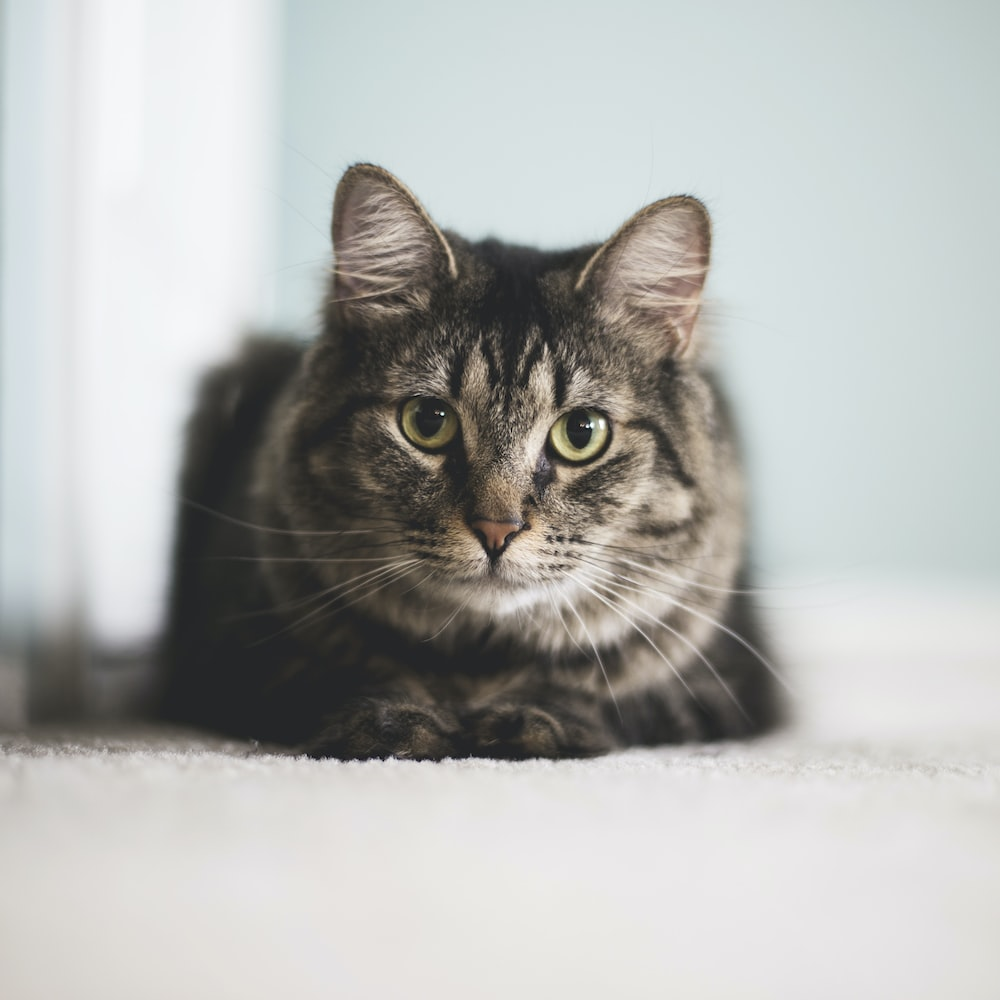
\includegraphics[width=1.5cm]{data/cat.jpeg}
			};
		\end{tikzpicture}
	\end{frame}

	\begin{frame}{The history of artificial intelligence} %DL (image classification)
		\begin{tikzpicture}
			\node[] at (0, 0) {};
			\node[] at (10.5, -7.5) {};

			\draw[very thick, gray] (0.5, -1)  -- (8.84, -1) {};

			\node[
				circle,
				draw=passivehistory,
				fill=passivehistory
			] at (1.65, -1) {};
			\node[
				anchor=north,
				passivehistory,
				align=center,
				font=\small\linespread{0.9}\selectfont,
				text height=9pt,
				text depth=3pt,
				inner sep=0pt,
				align=center
			] at (1.65, -1.588) {Turing\\test\\(1950)};

			\node[
				circle,
				draw=passivehistory,
				fill=passivehistory,
			] at (2.35, -1) {};
			\node[
				anchor=south,
				passivehistory,
				font=\small\linespread{0.9}\selectfont,
				text height=9pt,
				text depth=3pt,
				inner sep=0pt,
				align=center
			] at (2.35, -0.87) {Dartmouth\\(1956)};

			\node[
				circle,
				draw=passivehistory,
				fill=passivehistory,
			] at (2.68, -1) {};
			\node[
				anchor=north,
				passivehistory,
				font=\small\linespread{0.9}\selectfont,
				text height=9pt,
				text depth=3pt,
				inner sep=0pt,
				align=center
			] at (2.68, -1.375) {Perceptron\\(1958)};

			\node[
				circle,
				draw=passivehistory,
				fill=passivehistory
			] at (3.28, -1) {};
			\node[
				circle,
				draw=passivehistory,
				fill=passivehistory,
			] at (2.35, -1) {};
			\node[
				anchor=south,
				passivehistory,
				font=\small\linespread{0.9}\selectfont,
				text height=9pt,
				text depth=3pt,
				inner sep=0pt,
				align=center
			] at (3.28, -0.87) {Eliza\\(1964)};

			\node[
				circle,
				draw=passivehistory,
				fill=passivehistory
			] at (5.13, -1) {};
			\node[
				anchor=north,
				passivehistory,
				font=\small\linespread{0.9}\selectfont,
				text height=9pt,
				text depth=3pt,
				inner sep=0pt,
				align=center
			] at (5.13, -1.625) {Expert\\systems\\(1980s)};

			\node[
				circle,
				draw=passivehistory,
				fill=passivehistory
			] at (5.82, -1) {};
			\node[
				anchor=south,
				passivehistory,
				font=\small\linespread{0.9}\selectfont,
				text height=9pt,
				text depth=3pt,
				inner sep=0pt,
				align=center
			] at (5.82, -0.87) {ANNs\\(1986)};

			\node[
				circle,
				draw=passivehistory,
				fill=passivehistory
			] at (7.10, -1) {};
			\node[
				anchor=north,
				passivehistory,
				font=\small\linespread{0.9}\selectfont,
				text height=9pt,
				text depth=3pt,
				inner sep=0pt,
				align=center
			] at (7.10, -1.372) {Deep blue\\(1997)};

			\node[
				circle,
				draw=activehistory,
				fill=activehistory
			] at (8.84, -1) {};
			\node[
				anchor=south,
				activehistory,
				font=\small\linespread{0.9}\selectfont,
				text height=9pt,
				text depth=3pt,
				inner sep=0pt,
				align=center
			] at (8.84, -0.87) {Deep learning\\(2012)};

			\node[inner sep=0pt, label=below:\small{Cat}] (img3) at (5.25, -4.75) {
				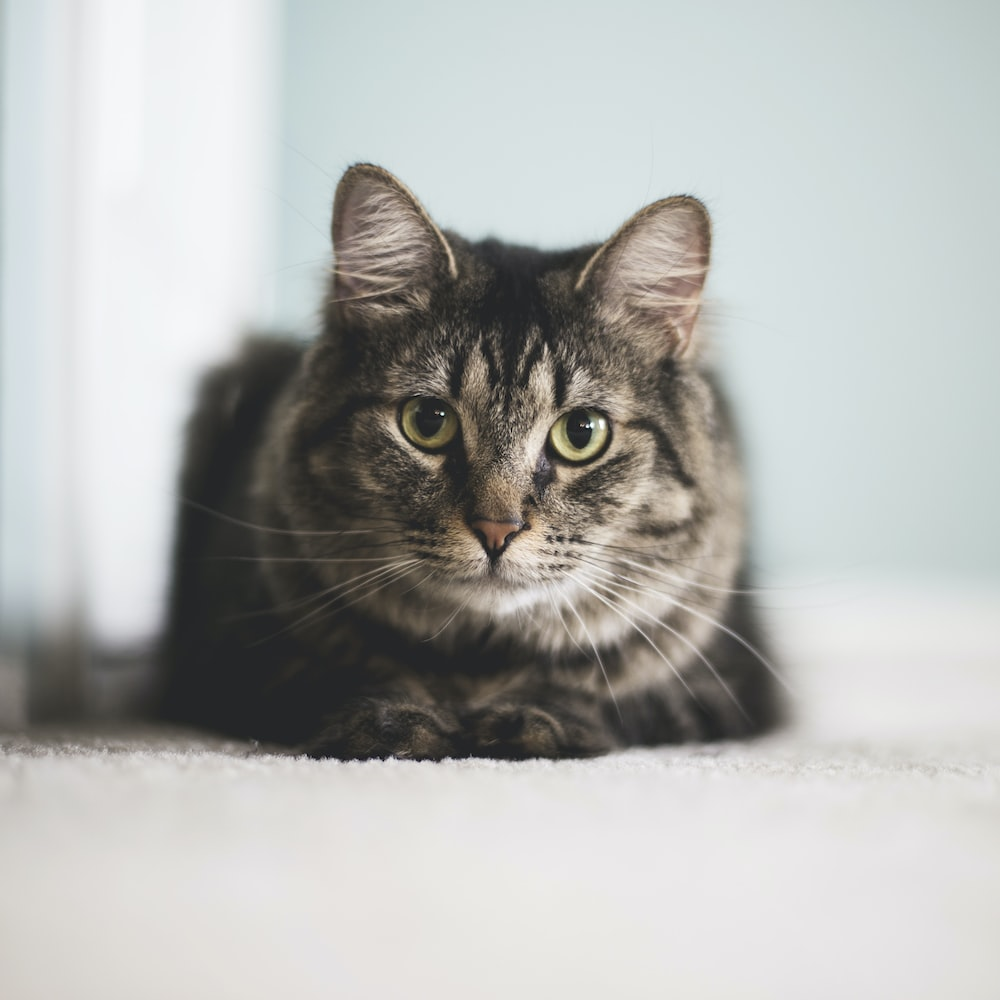
\includegraphics[width=1.5cm]{data/cat.jpeg}
			};
		\end{tikzpicture}
	\end{frame}

	\begin{frame}{The history of artificial intelligence} %DL (imagenet)
		\begin{tikzpicture}
			\node[] at (0, 0) {};
			\node[] at (10.5, -7.5) {};

			\draw[very thick, gray] (0.5, -1)  -- (8.84, -1) {};

			\node[
				circle,
				draw=passivehistory,
				fill=passivehistory
			] at (1.65, -1) {};
			\node[
				anchor=north,
				passivehistory,
				align=center,
				font=\small\linespread{0.9}\selectfont,
				text height=9pt,
				text depth=3pt,
				inner sep=0pt,
				align=center
			] at (1.65, -1.588) {Turing\\test\\(1950)};

			\node[
				circle,
				draw=passivehistory,
				fill=passivehistory,
			] at (2.35, -1) {};
			\node[
				anchor=south,
				passivehistory,
				font=\small\linespread{0.9}\selectfont,
				text height=9pt,
				text depth=3pt,
				inner sep=0pt,
				align=center
			] at (2.35, -0.87) {Dartmouth\\(1956)};

			\node[
				circle,
				draw=passivehistory,
				fill=passivehistory,
			] at (2.68, -1) {};
			\node[
				anchor=north,
				passivehistory,
				font=\small\linespread{0.9}\selectfont,
				text height=9pt,
				text depth=3pt,
				inner sep=0pt,
				align=center
			] at (2.68, -1.375) {Perceptron\\(1958)};

			\node[
				circle,
				draw=passivehistory,
				fill=passivehistory
			] at (3.28, -1) {};
			\node[
				circle,
				draw=passivehistory,
				fill=passivehistory,
			] at (2.35, -1) {};
			\node[
				anchor=south,
				passivehistory,
				font=\small\linespread{0.9}\selectfont,
				text height=9pt,
				text depth=3pt,
				inner sep=0pt,
				align=center
			] at (3.28, -0.87) {Eliza\\(1964)};

			\node[
				circle,
				draw=passivehistory,
				fill=passivehistory
			] at (5.13, -1) {};
			\node[
				anchor=north,
				passivehistory,
				font=\small\linespread{0.9}\selectfont,
				text height=9pt,
				text depth=3pt,
				inner sep=0pt,
				align=center
			] at (5.13, -1.625) {Expert\\systems\\(1980s)};

			\node[
				circle,
				draw=passivehistory,
				fill=passivehistory
			] at (5.82, -1) {};
			\node[
				anchor=south,
				passivehistory,
				font=\small\linespread{0.9}\selectfont,
				text height=9pt,
				text depth=3pt,
				inner sep=0pt,
				align=center
			] at (5.82, -0.87) {ANNs\\(1986)};

			\node[
				circle,
				draw=passivehistory,
				fill=passivehistory
			] at (7.10, -1) {};
			\node[
				anchor=north,
				passivehistory,
				font=\small\linespread{0.9}\selectfont,
				text height=9pt,
				text depth=3pt,
				inner sep=0pt,
				align=center
			] at (7.10, -1.372) {Deep blue\\(1997)};

			\node[
				circle,
				draw=activehistory,
				fill=activehistory
			] at (8.84, -1) {};
			\node[
				anchor=south,
				activehistory,
				font=\small\linespread{0.9}\selectfont,
				text height=9pt,
				text depth=3pt,
				inner sep=0pt,
				align=center
			] at (8.84, -0.87) {Deep learning\\(2012)};

			\node[inner sep=0pt, label=below:\small{Cat}] (img3) at (5.25, -4.75) {
				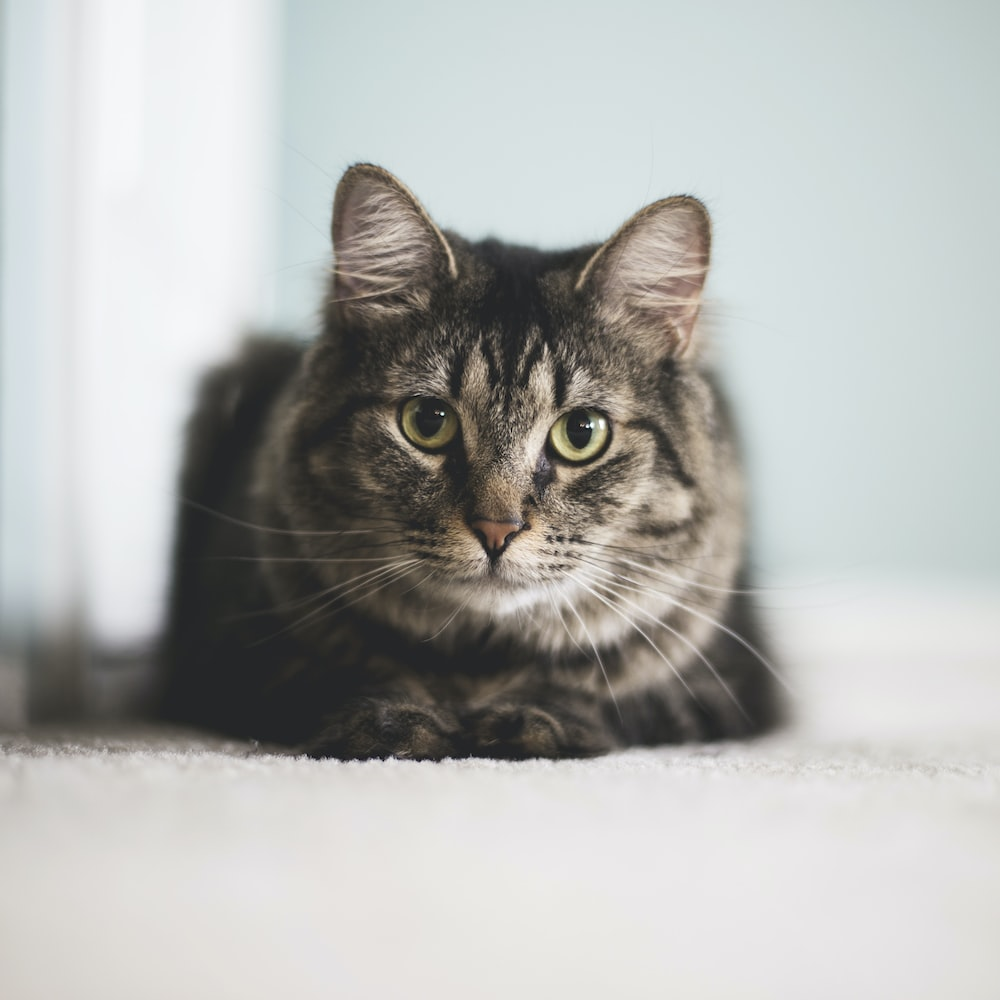
\includegraphics[width=1.5cm]{data/cat.jpeg}
			};
			\node[inner sep=0pt, label=below:\small{Airplane}, anchor=west] (img4) at ($ (img3.east) + (0.1, 0) $) {
				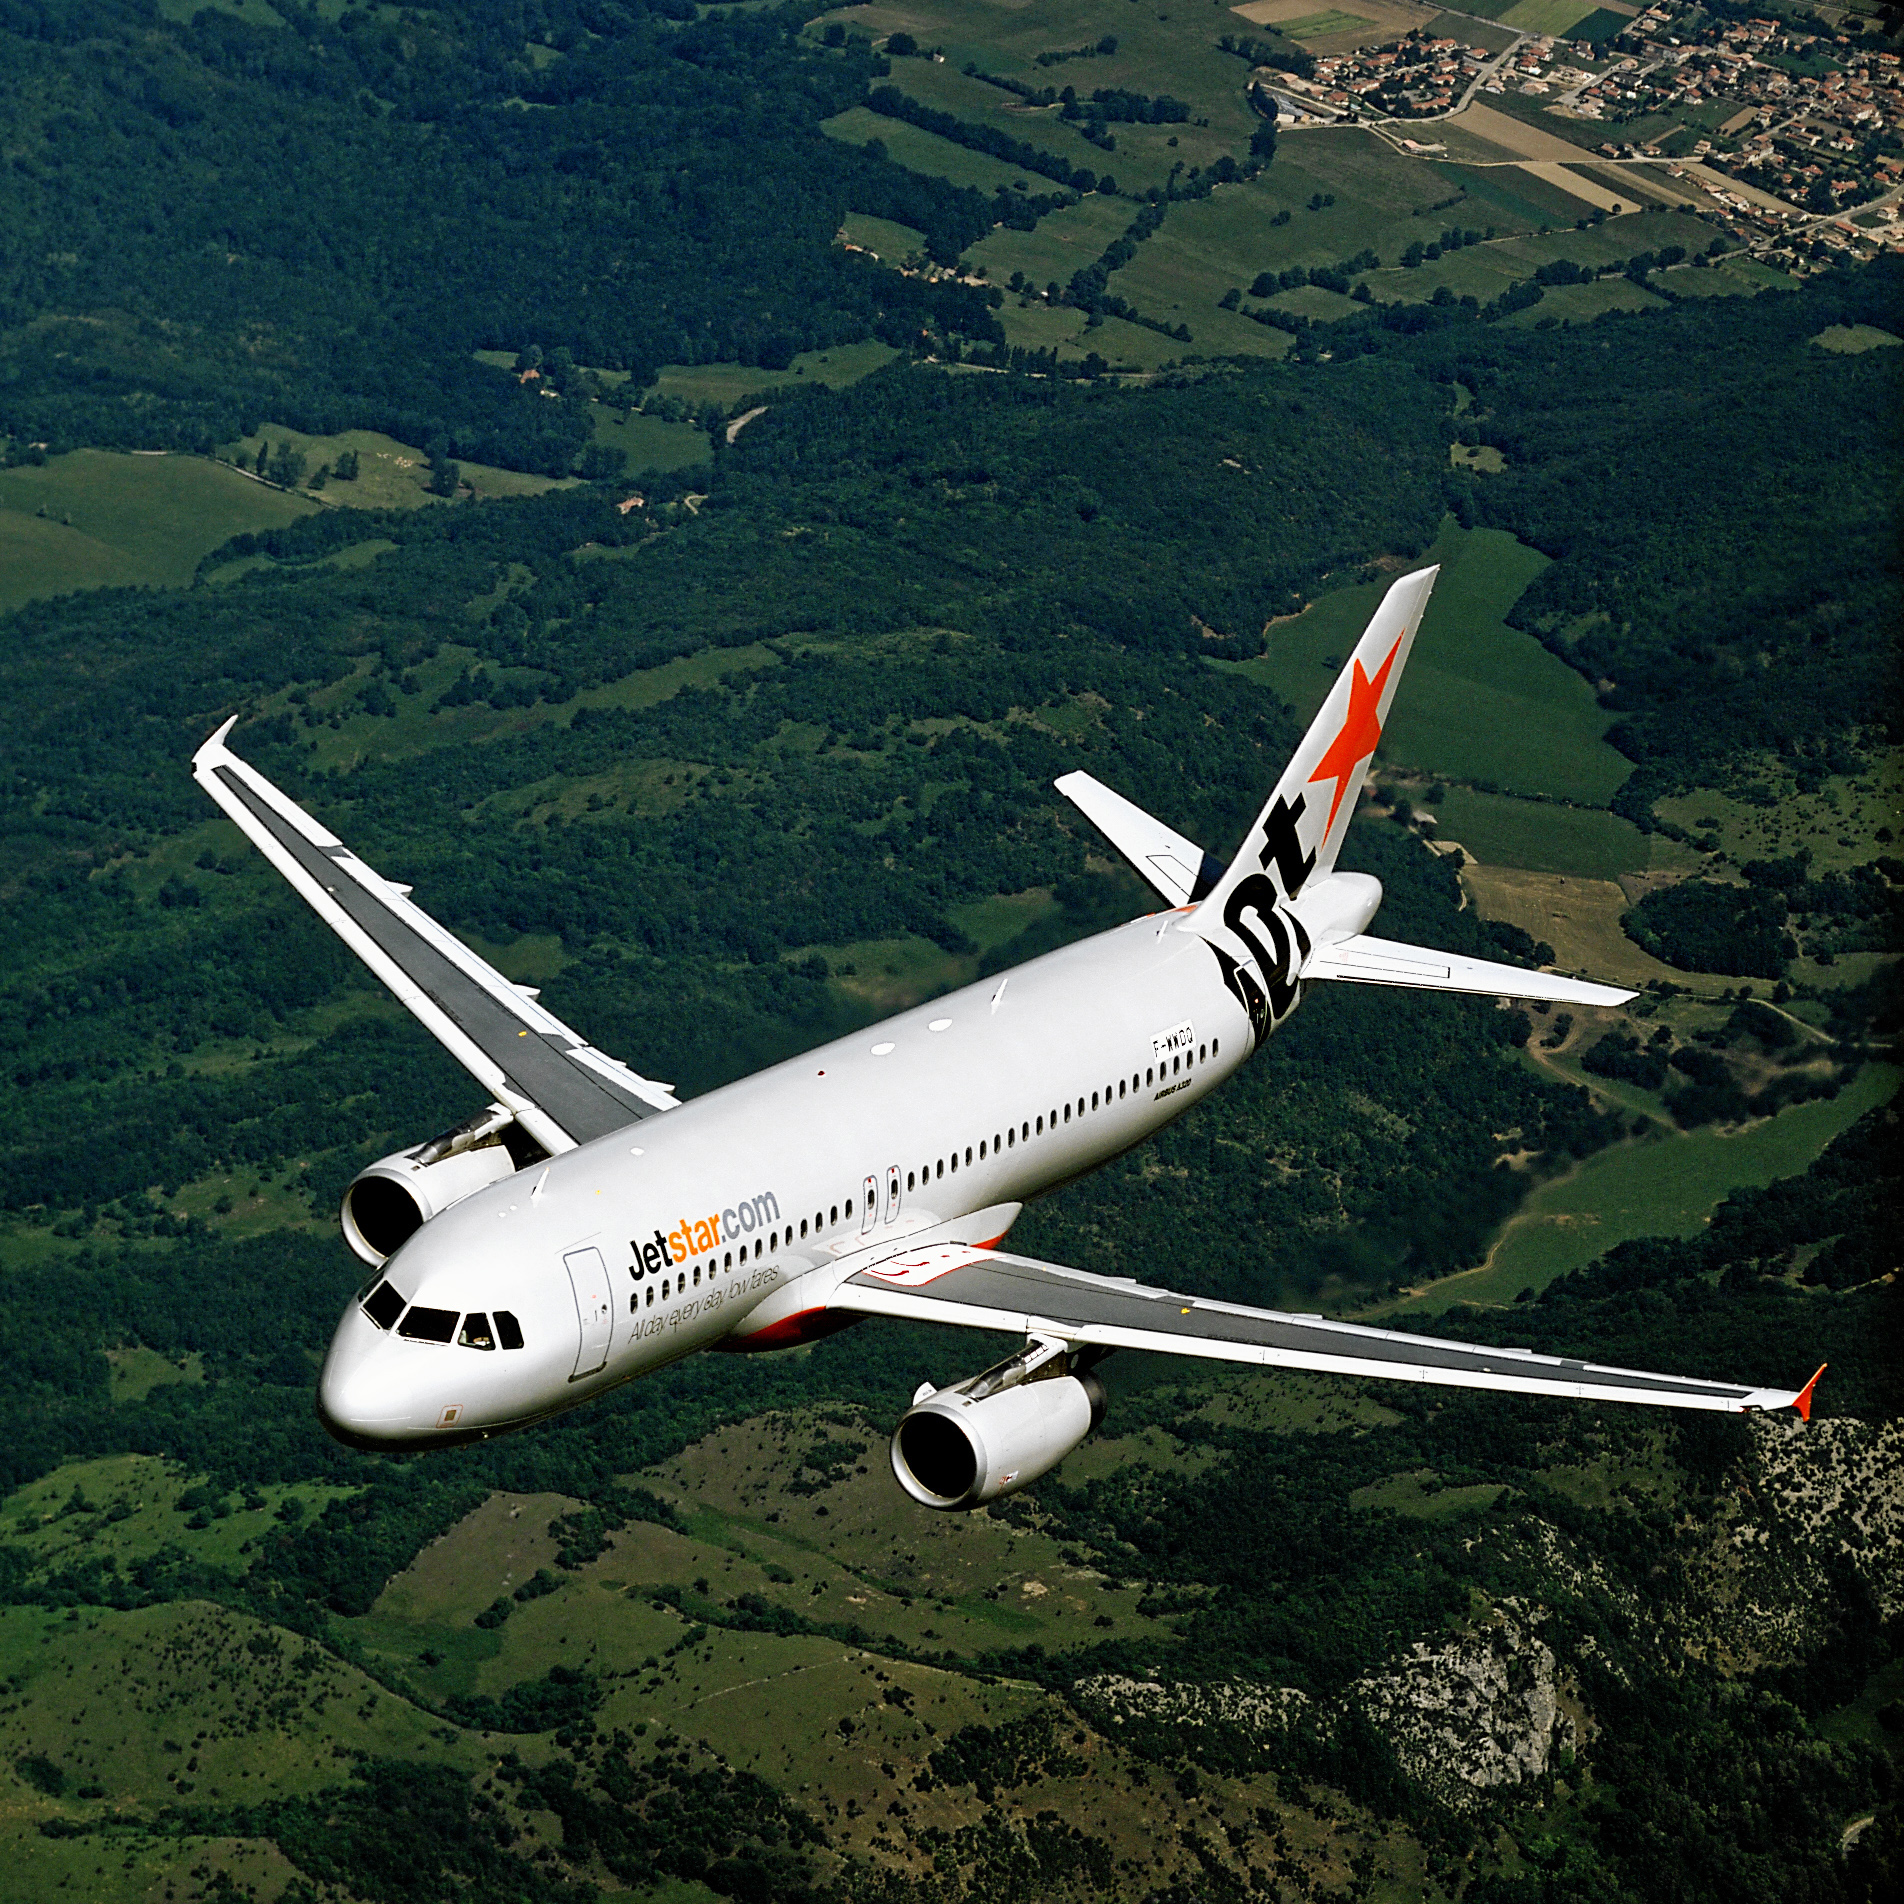
\includegraphics[width=1.5cm]{data/airplane.jpeg}
			};
			\node[inner sep=0pt, label=below:\small{Shark}, anchor=west] (img5) at ($ (img4.east) + (0.1, 0) $) {
				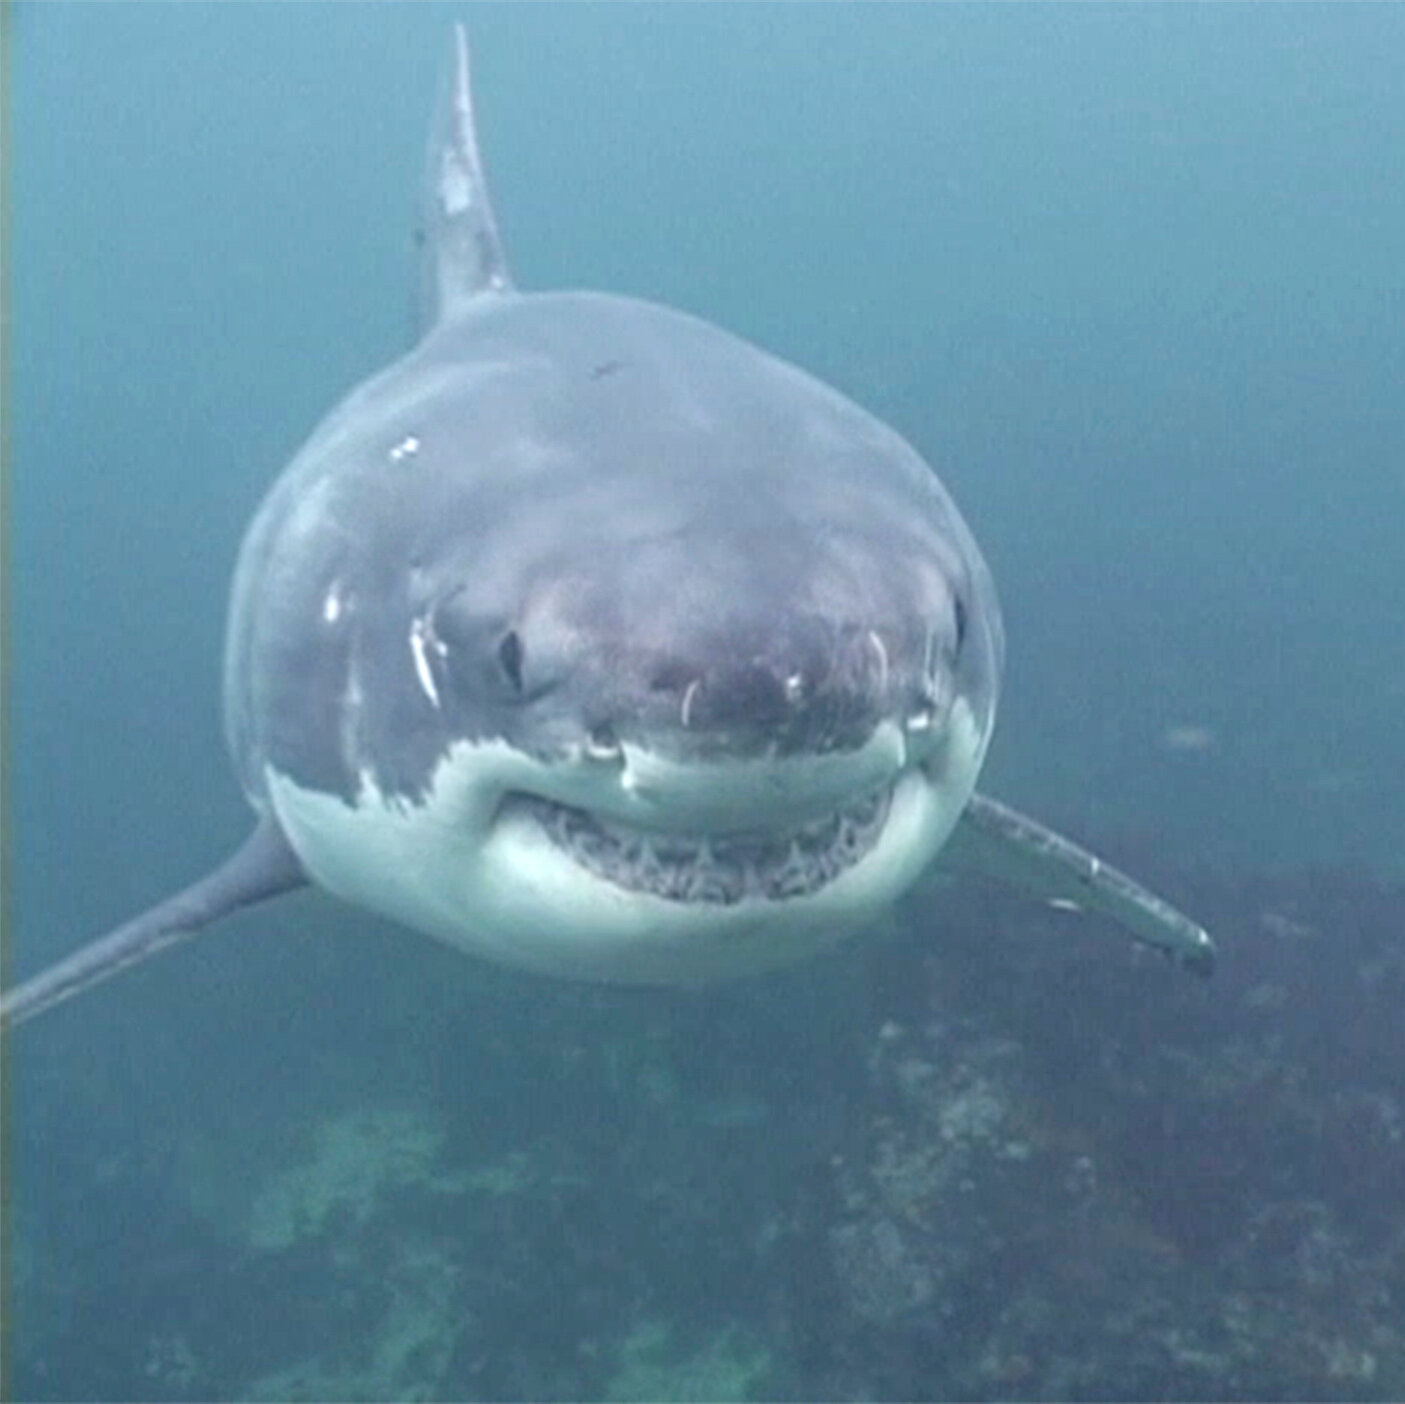
\includegraphics[width=1.5cm]{data/shark.jpeg}
			};
			\node[inner sep=0pt, label=below:\small{Ladybug}, anchor=east] (img2) at ($ (img3.west) - (0.1, 0) $) {
				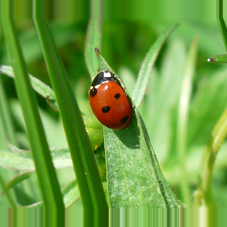
\includegraphics[width=1.5cm]{data/ladybug.png}
			};
			\node[inner sep=0pt, label=below:\small{Sunflower}, anchor=east] (img1) at ($ (img2.west) - (0.1, 0) $) {
				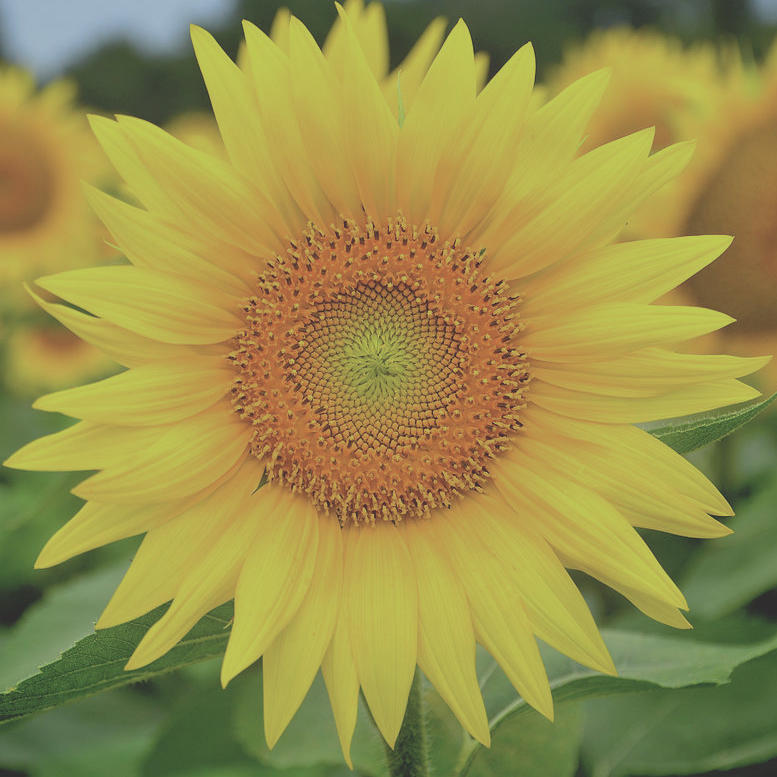
\includegraphics[width=1.5cm]{data/sunflower.jpeg}
			};
			\node[] at (5.25, -6.5) {
				ImageNet: $\sim$14m images, $\sim$22k categories
			};
		\end{tikzpicture}
	\end{frame}

	\begin{frame}{The history of artificial intelligence} %DL (old)
		\newsavebox{\imagenetold}
		\sbox{\imagenetold}{%
			\begin{tikzpicture}
				\begin{axis}[
					ylabel={Error rate},
					xlabel={Year},
					xtick={2010, 2012, 2014, 2016, 2018, 2020},
					xticklabels={2010, 2012, 2014, 2016, 2018, 2020},
					ytick={0, 10, 20, 30},
					yticklabels={0\%, 10\%, 20\%, 30\%},
					ytick style={draw=none},
					ytick pos=left,
					xtick pos=bottom,
					ymajorgrids=true,
					ymax=29,
					ymin=0,
					xmin=2009,
					xmax=2021,
					width=8cm,
					height=5cm
				]
					\addplot[mark=*, purple,thick] coordinates {
						(2010, 28.2)
						(2011, 25.8)
					};

					\node[anchor=north, inner sep=5pt] at (axis cs: 2010, 28.2) {
						\small{28.2}
					};
					\node[anchor=north, inner sep=5pt] at (axis cs: 2011, 25.8) {
						\small{25.8}
					};
				\end{axis}
			\end{tikzpicture}
		}

		\begin{tikzpicture}
			\node[] at (0, 0) {};
			\node[] at (10.5, -7.5) {};

			\draw[very thick, gray] (0.5, -1)  -- (8.84, -1) {};

			\node[
				circle,
				draw=passivehistory,
				fill=passivehistory
			] at (1.65, -1) {};
			\node[
				anchor=north,
				passivehistory,
				align=center,
				font=\small\linespread{0.9}\selectfont,
				text height=9pt,
				text depth=3pt,
				inner sep=0pt,
				align=center
			] at (1.65, -1.588) {Turing\\test\\(1950)};

			\node[
				circle,
				draw=passivehistory,
				fill=passivehistory,
			] at (2.35, -1) {};
			\node[
				anchor=south,
				passivehistory,
				font=\small\linespread{0.9}\selectfont,
				text height=9pt,
				text depth=3pt,
				inner sep=0pt,
				align=center
			] at (2.35, -0.87) {Dartmouth\\(1956)};

			\node[
				circle,
				draw=passivehistory,
				fill=passivehistory,
			] at (2.68, -1) {};
			\node[
				anchor=north,
				passivehistory,
				font=\small\linespread{0.9}\selectfont,
				text height=9pt,
				text depth=3pt,
				inner sep=0pt,
				align=center
			] at (2.68, -1.375) {Perceptron\\(1958)};

			\node[
				circle,
				draw=passivehistory,
				fill=passivehistory
			] at (3.28, -1) {};
			\node[
				circle,
				draw=passivehistory,
				fill=passivehistory,
			] at (2.35, -1) {};
			\node[
				anchor=south,
				passivehistory,
				font=\small\linespread{0.9}\selectfont,
				text height=9pt,
				text depth=3pt,
				inner sep=0pt,
				align=center
			] at (3.28, -0.87) {Eliza\\(1964)};

			\node[
				circle,
				draw=passivehistory,
				fill=passivehistory
			] at (5.13, -1) {};
			\node[
				anchor=north,
				passivehistory,
				font=\small\linespread{0.9}\selectfont,
				text height=9pt,
				text depth=3pt,
				inner sep=0pt,
				align=center
			] at (5.13, -1.625) {Expert\\systems\\(1980s)};

			\node[
				circle,
				draw=passivehistory,
				fill=passivehistory
			] at (5.82, -1) {};
			\node[
				anchor=south,
				passivehistory,
				font=\small\linespread{0.9}\selectfont,
				text height=9pt,
				text depth=3pt,
				inner sep=0pt,
				align=center
			] at (5.82, -0.87) {ANNs\\(1986)};

			\node[
				circle,
				draw=passivehistory,
				fill=passivehistory
			] at (7.10, -1) {};
			\node[
				anchor=north,
				passivehistory,
				font=\small\linespread{0.9}\selectfont,
				text height=9pt,
				text depth=3pt,
				inner sep=0pt,
				align=center
			] at (7.10, -1.372) {Deep blue\\(1997)};

			\node[
				circle,
				draw=activehistory,
				fill=activehistory
			] at (8.84, -1) {};
			\node[
				anchor=south,
				activehistory,
				font=\small\linespread{0.9}\selectfont,
				text height=9pt,
				text depth=3pt,
				inner sep=0pt,
				align=center
			] at (8.84, -0.87) {Deep learning\\(2012)};

			\node[inner sep=0pt] at (5.25, -4.75) {
				\usebox{\imagenetold}
			};
		\end{tikzpicture}
	\end{frame}

	\begin{frame}{The history of artificial intelligence} %DL (CNN)
		\newsavebox{\imagenetcnn}
		\sbox{\imagenetcnn}{%
			\begin{tikzpicture}
				\begin{axis}[
					ylabel={Error rate},
					xlabel={Year},
					xtick={2010, 2012, 2014, 2016, 2018, 2020},
					xticklabels={2010, 2012, 2014, 2016, 2018, 2020},
					ytick={0, 10, 20, 30},
					yticklabels={0\%, 10\%, 20\%, 30\%},
					ytick style={draw=none},
					ytick pos=left,
					xtick pos=bottom,
					ymajorgrids=true,
					ymax=29,
					ymin=0,
					xmin=2009,
					xmax=2021,
					width=8cm,
					height=5cm
				]
					\addplot[mark=*, purple,thick] coordinates {
						(2010, 28.2)
						(2011, 25.8)
						(2012, 16.4)
					};

					\node[anchor=north, inner sep=5pt] at (axis cs: 2010, 28.2) {
						\small{28.2}
					};
					\node[anchor=north, inner sep=5pt] at (axis cs: 2011, 25.8) {
						\small{25.8}
					};
					\node[anchor=north, inner sep=5pt] at (axis cs: 2012, 16.4) {
						\small{16.4}
					};

					\addplot[densely dotted] coordinates {
						(2011.5, 30)
						(2011.5, 0)
					};
				\end{axis}
			\end{tikzpicture}
		}

		\begin{tikzpicture}
			\node[] at (0, 0) {};
			\node[] at (10.5, -7.5) {};

			\draw[very thick, gray] (0.5, -1)  -- (8.84, -1) {};

			\node[
				circle,
				draw=passivehistory,
				fill=passivehistory
			] at (1.65, -1) {};
			\node[
				anchor=north,
				passivehistory,
				align=center,
				font=\small\linespread{0.9}\selectfont,
				text height=9pt,
				text depth=3pt,
				inner sep=0pt,
				align=center
			] at (1.65, -1.588) {Turing\\test\\(1950)};

			\node[
				circle,
				draw=passivehistory,
				fill=passivehistory,
			] at (2.35, -1) {};
			\node[
				anchor=south,
				passivehistory,
				font=\small\linespread{0.9}\selectfont,
				text height=9pt,
				text depth=3pt,
				inner sep=0pt,
				align=center
			] at (2.35, -0.87) {Dartmouth\\(1956)};

			\node[
				circle,
				draw=passivehistory,
				fill=passivehistory,
			] at (2.68, -1) {};
			\node[
				anchor=north,
				passivehistory,
				font=\small\linespread{0.9}\selectfont,
				text height=9pt,
				text depth=3pt,
				inner sep=0pt,
				align=center
			] at (2.68, -1.375) {Perceptron\\(1958)};

			\node[
				circle,
				draw=passivehistory,
				fill=passivehistory
			] at (3.28, -1) {};
			\node[
				circle,
				draw=passivehistory,
				fill=passivehistory,
			] at (2.35, -1) {};
			\node[
				anchor=south,
				passivehistory,
				font=\small\linespread{0.9}\selectfont,
				text height=9pt,
				text depth=3pt,
				inner sep=0pt,
				align=center
			] at (3.28, -0.87) {Eliza\\(1964)};

			\node[
				circle,
				draw=passivehistory,
				fill=passivehistory
			] at (5.13, -1) {};
			\node[
				anchor=north,
				passivehistory,
				font=\small\linespread{0.9}\selectfont,
				text height=9pt,
				text depth=3pt,
				inner sep=0pt,
				align=center
			] at (5.13, -1.625) {Expert\\systems\\(1980s)};

			\node[
				circle,
				draw=passivehistory,
				fill=passivehistory
			] at (5.82, -1) {};
			\node[
				anchor=south,
				passivehistory,
				font=\small\linespread{0.9}\selectfont,
				text height=9pt,
				text depth=3pt,
				inner sep=0pt,
				align=center
			] at (5.82, -0.87) {ANNs\\(1986)};

			\node[
				circle,
				draw=passivehistory,
				fill=passivehistory
			] at (7.10, -1) {};
			\node[
				anchor=north,
				passivehistory,
				font=\small\linespread{0.9}\selectfont,
				text height=9pt,
				text depth=3pt,
				inner sep=0pt,
				align=center
			] at (7.10, -1.372) {Deep blue\\(1997)};

			\node[
				circle,
				draw=activehistory,
				fill=activehistory
			] at (8.84, -1) {};
			\node[
				anchor=south,
				activehistory,
				font=\small\linespread{0.9}\selectfont,
				text height=9pt,
				text depth=3pt,
				inner sep=0pt,
				align=center
			] at (8.84, -0.87) {Deep learning\\(2012)};

			\node[inner sep=0pt] at (5.25, -4.75) {
				\usebox{\imagenetcnn}
			};
		\end{tikzpicture}
	\end{frame}

	\begin{frame}{The history of artificial intelligence} %DL (2020)
		\newsavebox{\imagenetlatest}
		\sbox{\imagenetlatest}{%
			\begin{tikzpicture}
				\begin{axis}[
					ylabel={Error rate},
					xlabel={Year},
					xtick={2010, 2012, 2014, 2016, 2018, 2020},
					xticklabels={2010, 2012, 2014, 2016, 2018, 2020},
					ytick={0, 10, 20, 30},
					yticklabels={0\%, 10\%, 20\%, 30\%},
					ytick style={draw=none},
					ytick pos=left,
					xtick pos=bottom,
					ymajorgrids=true,
					ymax=29,
					ymin=0,
					xmin=2009,
					xmax=2021,
					width=8cm,
					height=5cm
				]
					\addplot[mark=*, purple,thick] coordinates {
						(2010, 28.2)
						(2011, 25.8)
						(2012, 16.4)
						(2013, 11.7)
						(2014, 7.3)
						(2015, 3.5)
						(2016, 3.0)
						(2017, 2.3)
						(2018, 1.8)
						(2019, 1.3)
						(2020, 0.9)
					};

					\node[anchor=north, inner sep=5pt] at (axis cs: 2010, 28.2) {
						\small{28.2}
					};
					\node[anchor=north, inner sep=5pt] at (axis cs: 2011, 25.8) {
						\small{25.8}
					};
					\node[anchor=north, inner sep=5pt] at (axis cs: 2012, 16.4) {
						\small{16.4}
					};
					\node[anchor=north, inner sep=5pt] at (axis cs: 2013, 11.7) {
						\small{11.7}
					};
					\node[anchor=north, inner sep=5pt] at (axis cs: 2014, 7.3) {
						\small{7.3}
					};
					\node[anchor=north, inner sep=5pt] at (axis cs: 2015, 3.5) {
						\small{3.5}
					};
					\node[anchor=south, inner sep=5pt] at (axis cs: 2016, 3.0) {
						\small{3.0}
					};
					\node[anchor=south, inner sep=5pt] at (axis cs: 2017, 2.3) {
						\small{2.3}
					};
					\node[anchor=south, inner sep=5pt] at (axis cs: 2018, 1.8) {
						\small{1.8}
					};
					\node[anchor=south, inner sep=5pt] at (axis cs: 2019, 1.3) {
						\small{1.3}
					};
					\node[anchor=south, inner sep=5pt] at (axis cs: 2020, 0.9) {
						\small{\textbf{0.9}}
					};

					\addplot[densely dotted] coordinates {
						(2011.5, 30)
						(2011.5, 0)
					};
				\end{axis}
			\end{tikzpicture}
		}

		\begin{tikzpicture}
			\node[] at (0, 0) {};
			\node[] at (10.5, -7.5) {};

			\draw[very thick, gray] (0.5, -1)  -- (8.84, -1) {};

			\node[
				circle,
				draw=passivehistory,
				fill=passivehistory
			] at (1.65, -1) {};
			\node[
				anchor=north,
				passivehistory,
				align=center,
				font=\small\linespread{0.9}\selectfont,
				text height=9pt,
				text depth=3pt,
				inner sep=0pt,
				align=center
			] at (1.65, -1.588) {Turing\\test\\(1950)};

			\node[
				circle,
				draw=passivehistory,
				fill=passivehistory,
			] at (2.35, -1) {};
			\node[
				anchor=south,
				passivehistory,
				font=\small\linespread{0.9}\selectfont,
				text height=9pt,
				text depth=3pt,
				inner sep=0pt,
				align=center
			] at (2.35, -0.87) {Dartmouth\\(1956)};

			\node[
				circle,
				draw=passivehistory,
				fill=passivehistory,
			] at (2.68, -1) {};
			\node[
				anchor=north,
				passivehistory,
				font=\small\linespread{0.9}\selectfont,
				text height=9pt,
				text depth=3pt,
				inner sep=0pt,
				align=center
			] at (2.68, -1.375) {Perceptron\\(1958)};

			\node[
				circle,
				draw=passivehistory,
				fill=passivehistory
			] at (3.28, -1) {};
			\node[
				circle,
				draw=passivehistory,
				fill=passivehistory,
			] at (2.35, -1) {};
			\node[
				anchor=south,
				passivehistory,
				font=\small\linespread{0.9}\selectfont,
				text height=9pt,
				text depth=3pt,
				inner sep=0pt,
				align=center
			] at (3.28, -0.87) {Eliza\\(1964)};

			\node[
				circle,
				draw=passivehistory,
				fill=passivehistory
			] at (5.13, -1) {};
			\node[
				anchor=north,
				passivehistory,
				font=\small\linespread{0.9}\selectfont,
				text height=9pt,
				text depth=3pt,
				inner sep=0pt,
				align=center
			] at (5.13, -1.625) {Expert\\systems\\(1980s)};

			\node[
				circle,
				draw=passivehistory,
				fill=passivehistory
			] at (5.82, -1) {};
			\node[
				anchor=south,
				passivehistory,
				font=\small\linespread{0.9}\selectfont,
				text height=9pt,
				text depth=3pt,
				inner sep=0pt,
				align=center
			] at (5.82, -0.87) {ANNs\\(1986)};

			\node[
				circle,
				draw=passivehistory,
				fill=passivehistory
			] at (7.10, -1) {};
			\node[
				anchor=north,
				passivehistory,
				font=\small\linespread{0.9}\selectfont,
				text height=9pt,
				text depth=3pt,
				inner sep=0pt,
				align=center
			] at (7.10, -1.372) {Deep blue\\(1997)};

			\node[
				circle,
				draw=activehistory,
				fill=activehistory
			] at (8.84, -1) {};
			\node[
				anchor=south,
				activehistory,
				font=\small\linespread{0.9}\selectfont,
				text height=9pt,
				text depth=3pt,
				inner sep=0pt,
				align=center
			] at (8.84, -0.87) {Deep learning\\(2012)};

			\node[inner sep=0pt] at (5.25, -4.75) {
				\usebox{\imagenetlatest}
			};
		\end{tikzpicture}
	\end{frame}

	\begin{frame}{The history of artificial intelligence} %DL (human)
		\newsavebox{\imagenethuman}
		\sbox{\imagenethuman}{%
			\begin{tikzpicture}
				\begin{axis}[
					ylabel={Error rate},
					xlabel={Year},
					xtick={2010, 2012, 2014, 2016, 2018, 2020},
					xticklabels={2010, 2012, 2014, 2016, 2018, 2020},
					ytick={0, 10, 20, 30},
					yticklabels={0\%, 10\%, 20\%, 30\%},
					ytick style={draw=none},
					ytick pos=left,
					xtick pos=bottom,
					ymajorgrids=true,
					ymax=29,
					ymin=0,
					xmin=2009,
					xmax=2021,
					width=8cm,
					height=5cm
				]
					\addplot[mark=*, purple,thick] coordinates {
						(2010, 28.2)
						(2011, 25.8)
						(2012, 16.4)
						(2013, 11.7)
						(2014, 7.3)
						(2015, 3.5)
						(2016, 3.0)
						(2017, 2.3)
						(2018, 1.8)
						(2019, 1.3)
						(2020, 0.9)
					};

					\node[anchor=north, inner sep=5pt] at (axis cs: 2010, 28.2) {
						\small{28.2}
					};
					\node[anchor=north, inner sep=5pt] at (axis cs: 2011, 25.8) {
						\small{25.8}
					};
					\node[anchor=north, inner sep=5pt] at (axis cs: 2012, 16.4) {
						\small{16.4}
					};
					\node[anchor=north, inner sep=5pt] at (axis cs: 2013, 11.7) {
						\small{11.7}
					};
					\node[anchor=north, inner sep=5pt] at (axis cs: 2014, 7.3) {
						\small{7.3}
					};
					\node[anchor=north, inner sep=5pt] at (axis cs: 2015, 3.5) {
						\small{3.5}
					};
					\node[anchor=south, inner sep=5pt] at (axis cs: 2016, 3.0) {
						\small{3.0}
					};
					\node[anchor=south, inner sep=5pt] at (axis cs: 2017, 2.3) {
						\small{2.3}
					};
					\node[anchor=south, inner sep=5pt] at (axis cs: 2018, 1.8) {
						\small{1.8}
					};
					\node[anchor=south, inner sep=5pt] at (axis cs: 2019, 1.3) {
						\small{1.3}
					};
					\node[anchor=south, inner sep=5pt] at (axis cs: 2020, 0.9) {
						\small{\textbf{0.9}}
					};

					\addplot[densely dotted] coordinates {
						(2011.5, 30)
						(2011.5, 0)
					};

					\addplot[dashed, red] coordinates {
						(2009, 5.1)
						(2021, 5.1)
					};

					\node[anchor=south east] at (axis cs: 2021, 5.1) {
						\textcolor{red}{\small{Human level}}
					};
				\end{axis}
			\end{tikzpicture}
		}

		\begin{tikzpicture}
			\node[] at (0, 0) {};
			\node[] at (10.5, -7.5) {};

			\draw[very thick, gray] (0.5, -1)  -- (8.84, -1) {};

			\node[
				circle,
				draw=passivehistory,
				fill=passivehistory
			] at (1.65, -1) {};
			\node[
				anchor=north,
				passivehistory,
				align=center,
				font=\small\linespread{0.9}\selectfont,
				text height=9pt,
				text depth=3pt,
				inner sep=0pt,
				align=center
			] at (1.65, -1.588) {Turing\\test\\(1950)};

			\node[
				circle,
				draw=passivehistory,
				fill=passivehistory,
			] at (2.35, -1) {};
			\node[
				anchor=south,
				passivehistory,
				font=\small\linespread{0.9}\selectfont,
				text height=9pt,
				text depth=3pt,
				inner sep=0pt,
				align=center
			] at (2.35, -0.87) {Dartmouth\\(1956)};

			\node[
				circle,
				draw=passivehistory,
				fill=passivehistory,
			] at (2.68, -1) {};
			\node[
				anchor=north,
				passivehistory,
				font=\small\linespread{0.9}\selectfont,
				text height=9pt,
				text depth=3pt,
				inner sep=0pt,
				align=center
			] at (2.68, -1.375) {Perceptron\\(1958)};

			\node[
				circle,
				draw=passivehistory,
				fill=passivehistory
			] at (3.28, -1) {};
			\node[
				circle,
				draw=passivehistory,
				fill=passivehistory,
			] at (2.35, -1) {};
			\node[
				anchor=south,
				passivehistory,
				font=\small\linespread{0.9}\selectfont,
				text height=9pt,
				text depth=3pt,
				inner sep=0pt,
				align=center
			] at (3.28, -0.87) {Eliza\\(1964)};

			\node[
				circle,
				draw=passivehistory,
				fill=passivehistory
			] at (5.13, -1) {};
			\node[
				anchor=north,
				passivehistory,
				font=\small\linespread{0.9}\selectfont,
				text height=9pt,
				text depth=3pt,
				inner sep=0pt,
				align=center
			] at (5.13, -1.625) {Expert\\systems\\(1980s)};

			\node[
				circle,
				draw=passivehistory,
				fill=passivehistory
			] at (5.82, -1) {};
			\node[
				anchor=south,
				passivehistory,
				font=\small\linespread{0.9}\selectfont,
				text height=9pt,
				text depth=3pt,
				inner sep=0pt,
				align=center
			] at (5.82, -0.87) {ANNs\\(1986)};

			\node[
				circle,
				draw=passivehistory,
				fill=passivehistory
			] at (7.10, -1) {};
			\node[
				anchor=north,
				passivehistory,
				font=\small\linespread{0.9}\selectfont,
				text height=9pt,
				text depth=3pt,
				inner sep=0pt,
				align=center
			] at (7.10, -1.372) {Deep blue\\(1997)};

			\node[
				circle,
				draw=activehistory,
				fill=activehistory
			] at (8.84, -1) {};
			\node[
				anchor=south,
				activehistory,
				font=\small\linespread{0.9}\selectfont,
				text height=9pt,
				text depth=3pt,
				inner sep=0pt,
				align=center
			] at (8.84, -0.87) {Deep learning\\(2012)};

			\node[inner sep=0pt] at (5.25, -4.75) {
				\usebox{\imagenethuman}
			};
		\end{tikzpicture}
	\end{frame}

	\begin{frame}{The history of artificial intelligence} %ChatGPT
		\begin{tikzpicture}
			\node[] at (0, 0) {};
			\node[] at (10.5, -7.5) {};

			\draw[very thick, gray] (0.5, -1)  -- (10, -1) {};

			\node[
				circle,
				draw=passivehistory,
				fill=passivehistory
			] at (1.65, -1) {};
			\node[
				anchor=north,
				passivehistory,
				align=center,
				font=\small\linespread{0.9}\selectfont,
				text height=9pt,
				text depth=3pt,
				inner sep=0pt,
				align=center
			] at (1.65, -1.588) {Turing\\test\\(1950)};

			\node[
				circle,
				draw=passivehistory,
				fill=passivehistory,
			] at (2.35, -1) {};
			\node[
				anchor=south,
				passivehistory,
				font=\small\linespread{0.9}\selectfont,
				text height=9pt,
				text depth=3pt,
				inner sep=0pt,
				align=center
			] at (2.35, -0.87) {Dartmouth\\(1956)};

			\node[
				circle,
				draw=passivehistory,
				fill=passivehistory,
			] at (2.68, -1) {};
			\node[
				anchor=north,
				passivehistory,
				font=\small\linespread{0.9}\selectfont,
				text height=9pt,
				text depth=3pt,
				inner sep=0pt,
				align=center
			] at (2.68, -1.375) {Perceptron\\(1958)};

			\node[
				circle,
				draw=passivehistory,
				fill=passivehistory
			] at (3.28, -1) {};
			\node[
				circle,
				draw=passivehistory,
				fill=passivehistory,
			] at (2.35, -1) {};
			\node[
				anchor=south,
				passivehistory,
				font=\small\linespread{0.9}\selectfont,
				text height=9pt,
				text depth=3pt,
				inner sep=0pt,
				align=center
			] at (3.28, -0.87) {Eliza\\(1964)};

			\node[
				circle,
				draw=passivehistory,
				fill=passivehistory
			] at (5.13, -1) {};
			\node[
				anchor=north,
				passivehistory,
				font=\small\linespread{0.9}\selectfont,
				text height=9pt,
				text depth=3pt,
				inner sep=0pt,
				align=center
			] at (5.13, -1.625) {Expert\\systems\\(1980s)};

			\node[
				circle,
				draw=passivehistory,
				fill=passivehistory
			] at (5.82, -1) {};
			\node[
				anchor=south,
				passivehistory,
				font=\small\linespread{0.9}\selectfont,
				text height=9pt,
				text depth=3pt,
				inner sep=0pt,
				align=center
			] at (5.82, -0.87) {ANNs\\(1986)};

			\node[
				circle,
				draw=passivehistory,
				fill=passivehistory
			] at (7.10, -1) {};
			\node[
				anchor=north,
				passivehistory,
				font=\small\linespread{0.9}\selectfont,
				text height=9pt,
				text depth=3pt,
				inner sep=0pt,
				align=center
			] at (7.10, -1.372) {Deep blue\\(1997)};

			\node[
				circle,
				draw=passivehistory,
				fill=passivehistory
			] at (8.84, -1) {};
			\node[
				anchor=south,
				passivehistory,
				font=\small\linespread{0.9}\selectfont,
				text height=9pt,
				text depth=3pt,
				inner sep=0pt,
				align=center
			] at (8.84, -0.87) {Deep learning\\(2012)};

			\node[
				circle,
				draw=activehistory,
				fill=activehistory
			] at (10, -1) {};
			\node[
				anchor=north,
				activehistory,
				font=\small\linespread{0.9}\selectfont,
				text height=9pt,
				text depth=3pt,
				inner sep=0pt,
				align=center
			] at (10, -1.33) {ChatGPT\\(2022)};

			\node[inner sep=0pt, draw=black] at (5.25, -4.75) {
				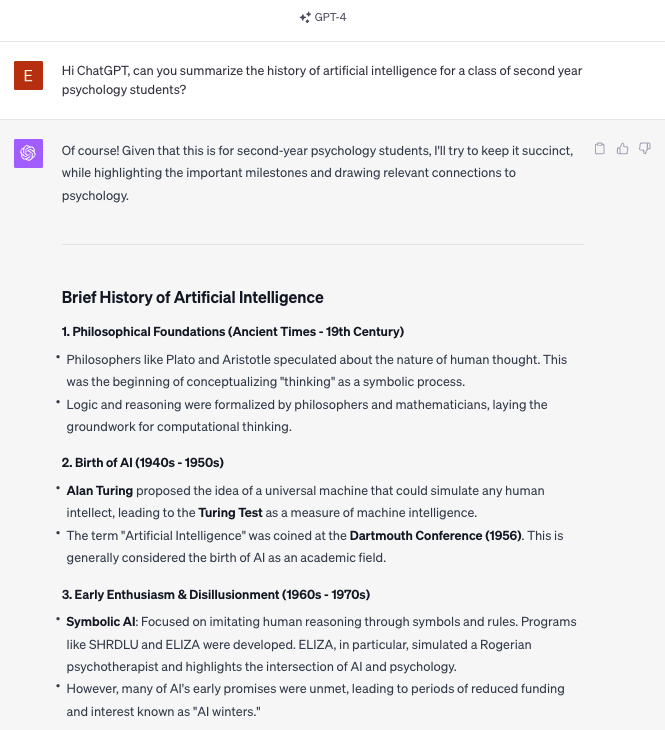
\includegraphics[width=4cm]{data/chatgpt.png}
			};
		\end{tikzpicture}
	\end{frame}

	% \section{Terminology and concepts}

	% \begin{frame}{Terminology and concepts: Taxonomy} % Taxonomy, Artificial intelligence
	% 	\centering
	% 	\vfill
	% 	\begin{tikzpicture}
	% 		\node[circle, fill=blue!60, minimum size=6cm] (ai) at (0, 0) {};
	% 		\node[text=white, anchor=north] at ($ (ai.north) - (0, 0.3) $) {\textbf{Artificial intelligence}};
	% 		\node[anchor=north west, align=left, font=\small] (ai-text) at ($ (ai.north) + (3.5, 0.2) $) {\textbf{Artificial intelligence:}\\Machines that solve tasks\\requiring intelligence};
	% 		\node[] at (-3, 3) {};
	% 		\node[] at (7.7, -3.2) {};
	% 	\end{tikzpicture}
	% 	\vfill
	% \end{frame}

	% \begin{frame}{Terminology and concepts: Taxonomy} % Taxonomy, Symbolic AI
	% 	\centering
	% 	\vfill
	% 	\begin{tikzpicture}
	% 		\node[circle, fill=blue!60, minimum size=6cm] (ai) at (0, 0) {};
	% 		\node[text=white, anchor=north] at ($ (ai.north) - (0, 0.3) $) {\textbf{Artificial intelligence}};
	% 		\node[text=white] at ($ (ai.north) - (-1.1, 1.2) $) {Symbolic AI};
	% 		\node[anchor=north west, align=left, font=\small, text=gray!40] (ai-text) at ($ (ai.north) + (3.5, 0.2) $) {\textbf{Artificial intelligence:}\\Machines that solve tasks\\requiring intelligence};

	% 		\node[] at (-3, 3) {};
	% 		\node[] at (7.7, -3.2) {};
	% 	\end{tikzpicture}
	% 	\vfill
	% \end{frame}

	% \begin{frame}{Terminology and concepts: Taxonomy} % Taxonomy, Machine learning explanation
	% 	\centering
	% 	\vfill
	% 	\begin{tikzpicture}
	% 		\node[circle, fill=blue!60, minimum size=6cm] (ai) at (0, 0) {};
	% 		\node[text=white, anchor=north] at ($ (ai.north) - (0, 0.3) $) {\textbf{Artificial intelligence}};
	% 		\node[text=white] at ($ (ai.north) - (-1.1, 1.2) $) {Symbolic AI};
	% 		\node[circle, fill=purple!60, minimum size=4.5cm, anchor=south] (ml) at ($ (ai.south) + (0, 0.05) $) {};
	% 		\node[text=white, anchor=north] at ($ (ml.north) - (0, 0.3) $) {\textbf{Machine learning}};
	% 		\node[anchor=north west, align=left, font=\small, text=gray!40] (ai-text) at ($ (ai.north) + (3.5, 0.2) $) {\textbf{Artificial intelligence:}\\Machines that solve tasks\\requiring intelligence};
	% 		\node[anchor=north west, align=left, font=\small] (ml-text) at ($ (ai-text.south west) - (0, 0) $) {\textbf{Machine learning:}\\Machines that learn to\\solve tasks through\\learning patterns from data};
	% 		\node[] at (-3, 3) {};
	% 		\node[] at (7.7, -3.2) {};
	% 	\end{tikzpicture}
	% 	\vfill
	% \end{frame}

	% \begin{frame}{Terminology and concepts: Taxonomy} % Taxonomy, Deep learning
	% 	\centering
	% 	\vfill
	% 	\begin{tikzpicture}
	% 		\node[circle, fill=blue!60, minimum size=6cm] (ai) at (0, 0) {};
	% 		\node[text=white, anchor=north] at ($ (ai.north) - (0, 0.3) $) {\textbf{Artificial intelligence}};
	% 		\node[text=white] at ($ (ai.north) - (-1.1, 1.2) $) {Symbolic AI};
	% 		\node[circle, fill=purple!60, minimum size=4.5cm, anchor=south] (ml) at ($ (ai.south) + (0, 0.05) $) {};
	% 		\node[text=white, anchor=north] at ($ (ml.north) - (0, 0.3) $) {\textbf{Machine learning}};
	% 		\node[text=white, align=center, font=\linespread{0.5}\selectfont] at ($ (ml.north) - (1, 1.1) $) {Linear\\regression};
	% 		\node[anchor=north west, align=left, font=\small, text=gray!40] (ai-text) at ($ (ai.north) + (3.5, 0.2) $) {\textbf{Artificial intelligence:}\\Machines that solve tasks\\requiring intelligence};
	% 		\node[anchor=north west, align=left, font=\small, text=gray!40] (ml-text) at ($ (ai-text.south west) - (0, 0) $) {\textbf{Machine learning:}\\Machines that learn to\\solve tasks through\\learning patterns from data};

	% 		\node[] at (-3, 3) {};
	% 		\node[] at (7.7, -3.2) {};
	% 	\end{tikzpicture}
	% 	\vfill
	% \end{frame}

	% \begin{frame}{Terminology and concepts: Taxonomy} % Taxonomy, Deep learning
	% 	\centering
	% 	\vfill
	% 	\begin{tikzpicture}
	% 		\node[circle, fill=blue!60, minimum size=6cm] (ai) at (0, 0) {};
	% 		\node[text=white, anchor=north] at ($ (ai.north) - (0, 0.3) $) {\textbf{Artificial intelligence}};
	% 		\node[text=white] at ($ (ai.north) - (-1.1, 1.2) $) {Symbolic AI};
	% 		\node[circle, fill=purple!60, minimum size=4.5cm, anchor=south] (ml) at ($ (ai.south) + (0, 0.05) $) {};
	% 		\node[text=white, anchor=north] at ($ (ml.north) - (0, 0.3) $) {\textbf{Machine learning}};
	% 		\node[text=white, align=center, font=\linespread{0.5}\selectfont] at ($ (ml.north) - (1, 1.1) $) {Linear\\regression};
	% 		\node[circle, fill=red!60, minimum size=3cm, anchor=south] (dl) at ($ (ai.south) + (0, 0.1) $) {};
	% 		\node[text=white, anchor=north] at ($ (dl.north) - (0, 0.3) $) {\textbf{Deep learning}};
	% 		\node[anchor=north west, align=left, font=\small, text=gray!40] (ai-text) at ($ (ai.north) + (3.5, 0.2) $) {\textbf{Artificial intelligence:}\\Machines that solve tasks\\requiring intelligence};
	% 		\node[anchor=north west, align=left, font=\small, text=gray!40] (ml-text) at ($ (ai-text.south west) - (0, 0) $) {\textbf{Machine learning:}\\Machines that learn to\\solve tasks through\\learning patterns from data};
	% 		\node[anchor=north west, align=left, font=\small] (dl-text) at ($ (ml-text.south west) - (0, 0) $) {\textbf{Deep learning:}\\Machine learning models\\ organized in hierarchies\\($\approx$ deep neural networks)\\inspired by the brain};
	% 		\node[] at (-3, 3) {};
	% 		\node[] at (7.7, -3.2) {};
	% 	\end{tikzpicture}
	% 	\vfill
	% \end{frame}

	% \begin{frame}{Terminology and concepts: Taxonomy} % Taxonomy, CNNs and LLMs
	% 	\centering
	% 	\vfill
	% 	\begin{tikzpicture}
	% 		\node[circle, fill=blue!60, minimum size=6cm] (ai) at (0, 0) {};
	% 		\node[text=white, anchor=north] at ($ (ai.north) - (0, 0.3) $) {\textbf{Artificial intelligence}};
	% 		\node[text=white] at ($ (ai.north) - (-1.1, 1.2) $) {Symbolic AI};
	% 		\node[circle, fill=purple!60, minimum size=4.5cm, anchor=south] (ml) at ($ (ai.south) + (0, 0.05) $) {};
	% 		\node[text=white, anchor=north] at ($ (ml.north) - (0, 0.3) $) {\textbf{Machine learning}};
	% 		\node[text=white, align=center, font=\linespread{0.5}\selectfont] at ($ (ml.north) - (1, 1.1) $) {Linear\\regression};
	% 		\node[circle, fill=red!60, minimum size=3cm, anchor=south] (dl) at ($ (ai.south) + (0, 0.1) $) {};
	% 		\node[text=white, anchor=north] at ($ (dl.north) - (0, 0.3) $) {\textbf{Deep learning}};
	% 		\node[align=center, text=white, font=\linespread{0.5}\selectfont] at ($ (dl.north) - (-0.2, 1.2) $) {Convolutional\\neural networks};
	% 		\node[align=center, text=white, font=\linespread{0.5}\selectfont] at ($ (dl.north) - (0.2, 2.1) $) {Large language\\models};
	% 		\node[anchor=north west, align=left, font=\small, text=gray!40] (ai-text) at ($ (ai.north) + (3.5, 0.2) $) {\textbf{Artificial intelligence:}\\Machines that solve tasks\\requiring intelligence};
	% 		\node[anchor=north west, align=left, font=\small, text=gray!40] (ml-text) at ($ (ai-text.south west) - (0, 0) $) {\textbf{Machine learning:}\\Machines that learn to\\solve tasks through\\learning patterns from data};
	% 		\node[anchor=north west, align=left, font=\small, text=gray!40] (dl-text) at ($ (ml-text.south west) - (0, 0) $) {\textbf{Deep learning:}\\Machine learning models\\ organized in hierarchies\\($\approx$ deep neural networks)\\inspired by the brain};
	% 		\node[anchor=north west, align=left, font=\small] (cnn-text) at ($ (dl-text.south west) - (0, 0) $) {\textbf{Convolutional neural nets:}\\Neural networks for image\\data};
	% 		\node[anchor=north west, align=left, font=\small] at ($ (cnn-text.south west) - (0, 0) $) {\textbf{Large language models:}\\Neural networks for natural\\language (ChatGPT)};
	% 		\node[] at (-3, 3) {};
	% 		\node[] at (7.7, -3.2) {};
	% 	\end{tikzpicture}
	% 	\vfill
	% \end{frame}

	% \begin{frame}{Terminology: Supervision} % Supervised vs unsupervised
	% 	\centering
	% 	\vfill
	% 	\begin{tikzpicture}
	% 		\node[align=center, anchor=north] (supervised) at (0, 0) {Supervised learning};
	% 		\node[align=center, anchor=north] (unsupervised) at (7, 0) {Unsupervised learning};
	% 		\draw[] (3.5, 0) -- (3.5, -7.5);
	% 		\node[] (cat1) at ($ (supervised.south) + (-1, -0.8) $) {
	% 			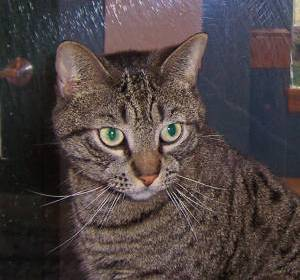
\includegraphics[width=1.2cm]{data/cat.1.jpg}
	% 		};
	% 		\node[anchor=west] (cattext1) at ($ (cat1.east) + (1.2, 0) $) {Cat};
	% 		\draw[->] (cat1) -- (cattext1);
	% 		\node[anchor=north] (dog1) at ($ (cat1.south) + (0, -0.1) $) {
	% 			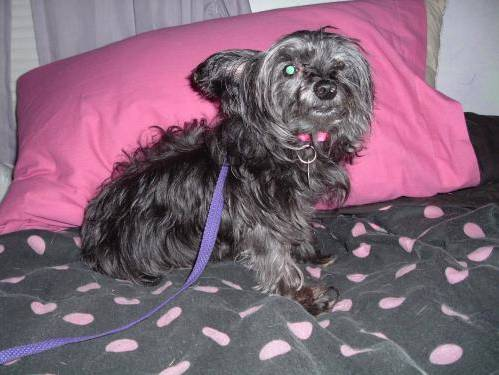
\includegraphics[width=1.2cm]{data/dog.0.jpg}
	% 		};
	% 		\node[anchor=west] (dogtext1) at ($ (dog1.east) + (1.2, 0) $) {Dog};
	% 		\draw[->] (dog1) -- (dogtext1);
	% 		\node[anchor=north] (cat2) at ($ (dog1.south) + (0, -0.1) $) {
	% 			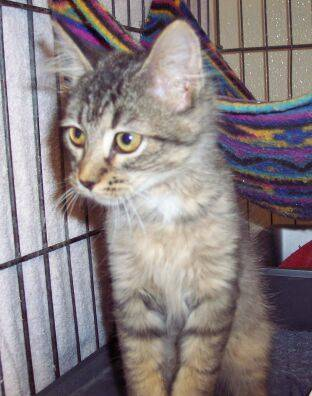
\includegraphics[width=1.2cm]{data/cat.2.jpg}
	% 		};
	% 		\node[anchor=west] (cattext2) at ($ (cat2.east) + (1.2, 0) $) {Cat};
	% 		\draw[->] (cat2) -- (cattext2);
	% 		\node[anchor=north] (dog2) at ($ (cat2.south) + (0, -0.1) $) {
	% 			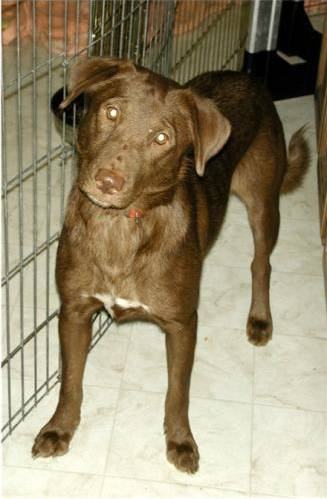
\includegraphics[width=1.2cm]{data/dog.1.jpg}
	% 		};
	% 		\node[anchor=west] (dogtext2) at ($ (dog2.east) + (1.2, 0) $) {Dog};
	% 		\draw[->] (dog2) -- (dogtext2);

	% 		\node[] (cat1) at ($ (unsupervised.south) + (-1.2, -2.4) $) {
	% 			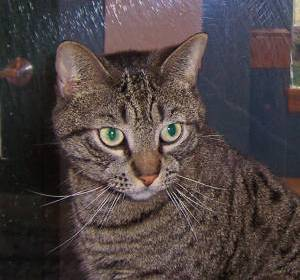
\includegraphics[width=0.8cm]{data/cat.1.jpg}
	% 		};
	% 		\node[] (cat2) at ($ (cat1) + (-0.9, 0.2) $) {
	% 			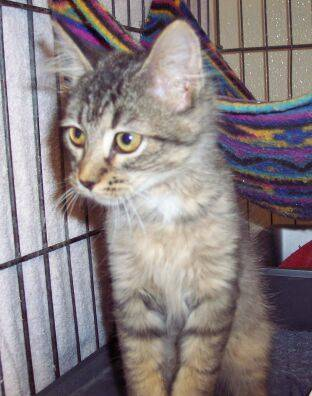
\includegraphics[width=0.8cm]{data/cat.2.jpg}
	% 		};
	% 		\node[] (cat3) at ($ (cat1) + (-0.5, -0.8) $) {
	% 			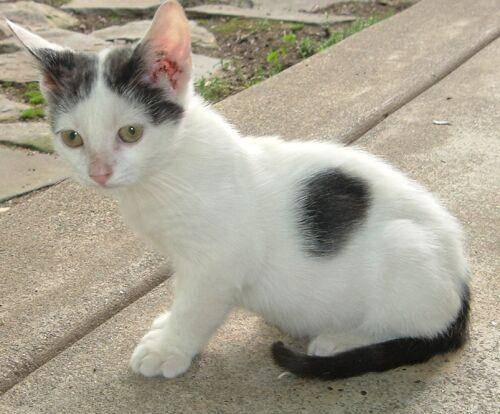
\includegraphics[width=0.8cm]{data/cat.3.jpg}
	% 		};
	% 		\node[] (cat4) at ($ (cat1) + (0.9, -0.1) $) {
	% 			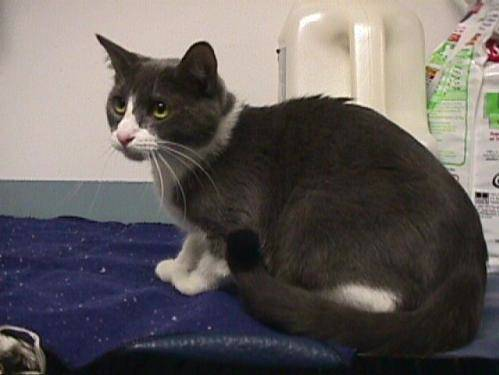
\includegraphics[width=0.8cm]{data/cat.4.jpg}
	% 		};

	% 		\node[] (dog1) at ($ (cat1) + (1.8, -1.5) $) {
	% 			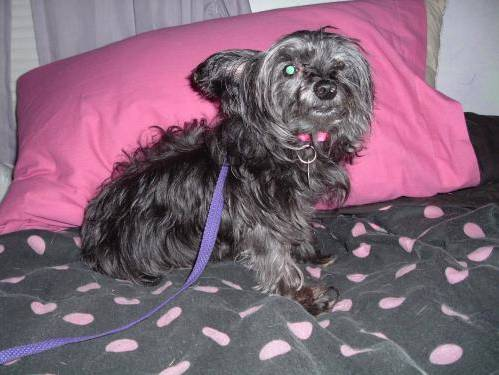
\includegraphics[width=0.8cm]{data/dog.0.jpg}
	% 		};
	% 		\node[] (dog2) at ($ (dog1) + (0.9, 0.1) $) {
	% 			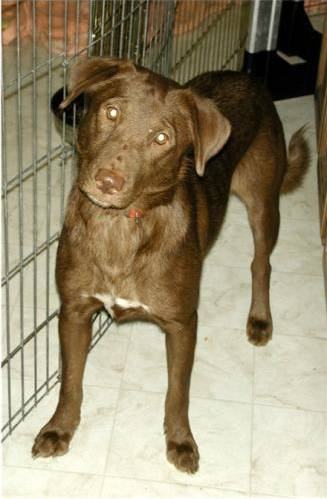
\includegraphics[width=0.8cm]{data/dog.1.jpg}
	% 		};
	% 		\node[] (dog3) at ($ (dog1) + (0.3, -0.8) $) {
	% 			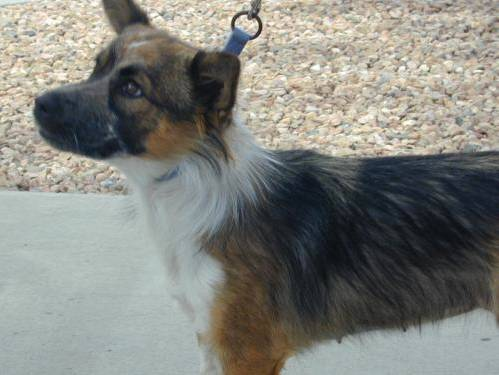
\includegraphics[width=0.8cm]{data/dog.3.jpg}
	% 		};
	% 		\node[] (dog4) at ($ (dog1) + (-0.9, -0.3) $) {
	% 			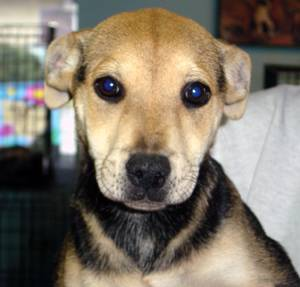
\includegraphics[width=0.8cm]{data/dog.4.jpg}
	% 		};
	% 		\draw[dashed, thick, red] ($ (cat1) + (-0.9, -1.7) $) -- ($ (dog1) + (1.2, 1.7) $);
	% 	\end{tikzpicture}
	% 	\vfill
	% \end{frame}

	% \begin{frame}{Terminology: Strong and weak AI} % Strong vs weak, axis
	% 	\centering
	% 	\vfill
	% 	\begin{tikzpicture}
	% 		\draw[<->] (0, 0) -- (10, 0);
	% 		\node[anchor=north west] at (0, -0.1) {More specific};
	% 		\node[anchor=north east] at (10, -0.1) {More general};
	% 		\node[anchor=north west] at (0, 6) {Narrow (weak)};
	% 		\node[anchor=north east] at (10, 6) {General (strong)};

	% 		\draw[red, ->, thick] (2, 4) -- (8, 4);
	% 		\node[anchor=south,align=center,text=red] at (5, 4.1) {Able to solve a broader spectrum of\\problems in a wider array of domains};

	% 		\node[] at (10.2, -0.4) {};
	% 		\node[] at (-0.2, 5.9) {};
	% 	\end{tikzpicture}
	% 	\vfill
	% \end{frame}

	% \begin{frame}{Terminology: Strong and weak AI} % Strong vs weak, dichotomi
	% 	\centering
	% 	\vfill
	% 	\begin{tikzpicture}
	% 		\draw[<->] (0, 0) -- (10, 0);
	% 		\node[anchor=north west] at (0, -0.1) {More specific};
	% 		\node[anchor=north east] at (10, -0.1) {More general};
	% 		\node[anchor=north west] at (0, 6) {Narrow (weak)};
	% 		\node[anchor=north east] at (10, 6) {General (strong)};

	% 		\draw[red, ->, thick] (2, 4) -- (8, 4);
	% 		\node[anchor=south,align=center,text=red] at (5, 4.1) {Able to solve a broader spectrum of\\problems in a wider array of domains};
	% 		\node[anchor=south east] at (9.5, 0.2) {
	% 			
\includegraphics[width=1.3cm]{data/human.png}
	% 		};
	% 		\node[anchor=south west] at (0.5, 0.2) {
	% 			
\includegraphics[width=1.3cm]{data/laptop.png}
	% 		};
	% 		\node[] at (10.2, -0.4) {};
	% 		\node[] at (-0.2, 5.9) {};
	% 	\end{tikzpicture}
	% 	\vfill
	% \end{frame}

	% \begin{frame}{Terminology: Strong and weak AI} % Strong vs weak, weak
	% 	\centering
	% 	\vfill
	% 	\begin{tikzpicture}
	% 		\draw[<->] (0, 0) -- (10, 0);
	% 		\node[anchor=north west] at (0, -0.1) {More specific};
	% 		\node[anchor=north east] at (10, -0.1) {More general};
	% 		\node[anchor=north west] at (0, 6) {Narrow (weak)};
	% 		\node[anchor=north east] at (10, 6) {General (strong)};

	% 		\draw[red, ->, thick] (2, 4) -- (8, 4);
	% 		\node[anchor=south,align=center,text=red] at (5, 4.1) {Able to solve a broader spectrum of\\problems in a wider array of domains};
	% 		\node[anchor=south east] at (9.5, 0.2) {
	% 			
\includegraphics[width=1.3cm]{data/human.png}
	% 		};
	% 		\node[anchor=south west] at (0.5, 0.2) {
	% 			
\includegraphics[width=1.3cm]{data/laptop.png}
	% 		};
	% 		\node[align=center,font=\small, fill=blue!60, text=white, minimum width=1.6cm, rounded corners=.1cm] at (3, 2.1) {
	% 			Image\\
	% 			diagnostics
	% 		};
	% 		\node[align=center,font=\small, fill=blue!60, text=white, minimum width=1.6cm, rounded corners=.1cm] at (3, 1.3) {
	% 			Insurance\\
	% 			pricing
	% 		};
	% 		\node[align=center,font=\small, fill=blue!60, text=white, minimum width=1.6cm, rounded corners=.1cm] at (3, 0.5) {
	% 			Document\\
	% 			reading
	% 		};
	% 		\node[] at (10.2, -0.4) {};
	% 		\node[] at (-0.2, 5.9) {};
	% 	\end{tikzpicture}
	% 	\vfill
	% \end{frame}

	% \begin{frame}{Terminology: Strong and weak AI} % Strong vs weak, stronger
	% 	\centering
	% 	\vfill
	% 	\begin{tikzpicture}
	% 		\draw[<->] (0, 0) -- (10, 0);
	% 		\node[anchor=north west] at (0, -0.1) {More specific};
	% 		\node[anchor=north east] at (10, -0.1) {More general};
	% 		\node[anchor=north west] at (0, 6) {Narrow (weak)};
	% 		\node[anchor=north east] at (10, 6) {General (strong)};

	% 		\draw[red, ->, thick] (2, 4) -- (8, 4);
	% 		\node[anchor=south,align=center,text=red] at (5, 4.1) {Able to solve a broader spectrum of\\problems in a wider array of domains};
	% 		\node[anchor=south east] at (9.5, 0.2) {
	% 			
\includegraphics[width=1.3cm]{data/human.png}
	% 		};
	% 		\node[anchor=south west] at (0.5, 0.2) {
	% 			
\includegraphics[width=1.3cm]{data/laptop.png}
	% 		};
	% 		\node[align=center,font=\small, fill=blue!60, text=white, minimum width=1.6cm, rounded corners=.1cm] at (3, 2.1) {
	% 			Image\\
	% 			diagnostics
	% 		};
	% 		\node[align=center,font=\small, fill=blue!60, text=white, minimum width=1.6cm, rounded corners=.1cm] at (3, 1.3) {
	% 			Insurance\\
	% 			pricing
	% 		};
	% 		\node[align=center,font=\small, fill=blue!60, text=white, minimum width=1.6cm, rounded corners=.1cm] at (3, 0.5) {
	% 			Document\\
	% 			reading
	% 		};
	% 		\node[align=center,font=\small, fill=blue!60, text=white, minimum width=1.6cm, rounded corners=.1cm] at (4.8, 0.5) {
	% 			Tesla
	% 		};
	% 		\node[align=center,font=\small, fill=blue!60, text=white, minimum width=1.6cm, rounded corners=.1cm] at (5.4, 1.1) {
	% 			ChatGPT
	% 		};
	% 		\node[] at (10.2, -0.4) {};
	% 		\node[] at (-0.2, 5.9) {};
	% 	\end{tikzpicture}
	% 	\vfill
	% \end{frame}

	% \section{How does AI make decisions?}

	% \begin{frame}{Decision making: Expert systems vs. machine learning} % Expert system
	% 	\begin{tikzpicture}
	% 		\node[draw=black, dashed] (in) at (-4, -0.75) {Laboratory report};

	% 		\node[draw=black, fill=background] (n00) at (0, 0) {
	% 			gram stain = gramneg
	% 		};
	% 		\node[draw=black, fill=background] (n01) at (0, -0.75) {
	% 			morphology = rod
	% 		};
	% 		\node[draw=black, fill=background] (n02) at (0, -1.5) {
	% 			aerobicity = anaerobic
	% 		};

	% 		\node[] (out) at (4, -0.75) {bacteroides};

	% 		\draw[-Latex] (in.east) -- (n00.west);
	% 		\draw[-Latex] (in.east) -- (n01.west);
	% 		\draw[-Latex] (in.east) -- (n02.west);
	% 		\draw[-Latex] (n00.east) -- (out.west);
	% 		\draw[-Latex] (n01.east) -- (out.west);
	% 		\draw[-Latex] (n02.east) -- (out.west);

	% 		\node[anchor=south west] at (-5.3, -2.2) {Expert system};

	% 		\node[] at (-5.3, 0.75) {};
	% 		\node[] at (5.3, -5.5) {};

	% 	\end{tikzpicture}
	% \end{frame}

	% \begin{frame}{Decision making: Expert systems vs. machine learning} % Black box
	% 	\begin{tikzpicture}
	% 		\node[draw=black, dashed] (in) at (-4, -0.75) {Laboratory report};

	% 		\node[draw=black, fill=background] (n00) at (0, 0) {
	% 			gram stain = gramneg
	% 		};
	% 		\node[draw=black, fill=background] (n01) at (0, -0.75) {
	% 			morphology = rod
	% 		};
	% 		\node[draw=black, fill=background] (n02) at (0, -1.5) {
	% 			aerobicity = anaerobic
	% 		};

	% 		\node[] (out) at (4, -0.75) {bacteroides};

	% 		\draw[-Latex] (in.east) -- (n00.west);
	% 		\draw[-Latex] (in.east) -- (n01.west);
	% 		\draw[-Latex] (in.east) -- (n02.west);
	% 		\draw[-Latex] (n00.east) -- (out.west);
	% 		\draw[-Latex] (n01.east) -- (out.west);
	% 		\draw[-Latex] (n02.east) -- (out.west);

	% 		\draw[fill=background] (-1.85, -2.65) rectangle (1.85, -5.35);

	% 		\node[draw=black, dashed] (in) at (-4, -4) {Laboratory report};

	% 		\node[] (out) at (4, -4) {bacteroides};

	% 		\draw[-Latex] (in.east) -- (-1.85, -4);

	% 		\draw[-Latex] (1.85, -4) -- (out);

	% 		\draw[densely dotted] (-5.3, -2.2) -- (5.3, -2.2);
	% 		\node[anchor=south west] at (-5.3, -2.2) {Expert system};
	% 		\node[anchor=north west] at (-5.3, -2.2) {Machine learning};

	% 		\node[] at (-5.3, 0.75) {};
	% 		\node[] at (5.3, -5.5) {};

	% 	\end{tikzpicture}
	% \end{frame}

	% \begin{frame}{Decision making: Expert systems vs. machine learning} % Comparison
	% 	\begin{tikzpicture}
	% 		\node[draw=black, dashed] (in) at (-4, -0.75) {Laboratory report};

	% 		\node[draw=black, fill=background] (n00) at (0, 0) {
	% 			gram stain = gramneg
	% 		};
	% 		\node[draw=black, fill=background] (n01) at (0, -0.75) {
	% 			morphology = rod
	% 		};
	% 		\node[draw=black, fill=background] (n02) at (0, -1.5) {
	% 			aerobicity = anaerobic
	% 		};

	% 		\node[] (out) at (4, -0.75) {bacteroides};

	% 		\draw[-Latex] (in.east) -- (n00.west);
	% 		\draw[-Latex] (in.east) -- (n01.west);
	% 		\draw[-Latex] (in.east) -- (n02.west);
	% 		\draw[-Latex] (n00.east) -- (out.west);
	% 		\draw[-Latex] (n01.east) -- (out.west);
	% 		\draw[-Latex] (n02.east) -- (out.west);

	% 		\draw[fill=background] (-1.85, -2.65) rectangle (1.85, -5.35);
	% 		\node[anchor=north east] at (1.85, -2.65) {\small{Neural network}};

	% 		\node[draw=black, dashed] (in) at (-4, -4) {Laboratory report};

	% 		\node[draw=black, fill=nodefill, circle, inner sep=4pt] (n00) at (-1.5, -3) {};
	% 		\node[draw=black, fill=nodefill, circle, inner sep=4pt] (n01) at (-1.5, -3.5) {};
	% 		\node[draw=black, fill=nodefill, circle, inner sep=4pt] (n02) at (-1.5, -4) {};
	% 		\node[draw=black, fill=nodefill, circle, inner sep=4pt] (n03) at (-1.5, -4.5) {};
	% 		\node[draw=black, fill=nodefill, circle, inner sep=4pt] (n04) at (-1.5, -5) {};

	% 		\node[draw=black, fill=nodefill, circle, inner sep=4pt] (n10) at (-0.75, -3.25) {};
	% 		\node[draw=black, fill=nodefill, circle, inner sep=4pt] (n11) at (-0.75, -3.75) {};
	% 		\node[draw=black, fill=nodefill, circle, inner sep=4pt] (n12) at (-0.75, -4.25) {};
	% 		\node[draw=black, fill=nodefill, circle, inner sep=4pt] (n13) at (-0.75, -4.75) {};

	% 		\node[draw=black, fill=nodefill, circle, inner sep=4pt] (n20) at (0, -3.5) {};
	% 		\node[draw=black, fill=nodefill, circle, inner sep=4pt] (n21) at (0, -4) {};
	% 		\node[draw=black, fill=nodefill, circle, inner sep=4pt] (n22) at (0, -4.5) {};

	% 		\node[draw=black, fill=nodefill, circle, inner sep=4pt] (n30) at (0.75, -3.75) {};
	% 		\node[draw=black, fill=nodefill, circle, inner sep=4pt] (n31) at (0.75, -4.25) {};

	% 		\node[draw=black, fill=nodefill, circle, inner sep=4pt] (n40) at (1.5, -4) {};

	% 		\node[] (out) at (4, -4) {bacteroides};

	% 		\draw[-Latex] (in.east) -- (n00);
	% 		\draw[-Latex] (in.east) -- (n01);
	% 		\draw[-Latex] (in.east) -- (n02);
	% 		\draw[-Latex] (in.east) -- (n03);
	% 		\draw[-Latex] (in.east) -- (n04);

	% 		\draw[] (n00) -- (n10);
	% 		\draw[] (n00) -- (n11);
	% 		\draw[] (n00) -- (n12);
	% 		\draw[] (n00) -- (n13);
	% 		\draw[] (n01) -- (n10);
	% 		\draw[] (n01) -- (n11);
	% 		\draw[] (n01) -- (n12);
	% 		\draw[] (n01) -- (n13);
	% 		\draw[] (n02) -- (n10);
	% 		\draw[] (n02) -- (n11);
	% 		\draw[] (n02) -- (n12);
	% 		\draw[] (n02) -- (n13);
	% 		\draw[] (n03) -- (n10);
	% 		\draw[] (n03) -- (n11);
	% 		\draw[] (n03) -- (n12);
	% 		\draw[] (n03) -- (n13);
	% 		\draw[] (n04) -- (n10);
	% 		\draw[] (n04) -- (n11);
	% 		\draw[] (n04) -- (n12);
	% 		\draw[] (n04) -- (n13);

	% 		\draw[] (n10) -- (n20);
	% 		\draw[] (n10) -- (n21);
	% 		\draw[] (n10) -- (n22);
	% 		\draw[] (n11) -- (n20);
	% 		\draw[] (n11) -- (n21);
	% 		\draw[] (n11) -- (n22);
	% 		\draw[] (n12) -- (n20);
	% 		\draw[] (n12) -- (n21);
	% 		\draw[] (n12) -- (n22);
	% 		\draw[] (n13) -- (n20);
	% 		\draw[] (n13) -- (n21);
	% 		\draw[] (n13) -- (n22);

	% 		\draw[] (n20) -- (n30);
	% 		\draw[] (n20) -- (n31);
	% 		\draw[] (n21) -- (n30);
	% 		\draw[] (n21) -- (n31);
	% 		\draw[] (n22) -- (n30);
	% 		\draw[] (n22) -- (n31);

	% 		\draw[] (n30) -- (n40);
	% 		\draw[] (n31) -- (n40);

	% 		\draw[-Latex] (n40) -- (out);

	% 		\draw[densely dotted] (-5.3, -2.2) -- (5.3, -2.2);
	% 		\node[anchor=south west] at (-5.3, -2.2) {Expert system};
	% 		\node[anchor=north west] at (-5.3, -2.2) {Machine learning};

	% 		\node[] at (-5.3, 0.75) {};
	% 		\node[] at (5.3, -5.5) {};

	% 	\end{tikzpicture}
	% \end{frame}

	% \begin{frame}[t]{Decision making: Loss functions} % Loss definition
	% 	\vspace{2cm}
	% 	A loss function formalizes what we want the machine learning model to do:\\
	% \end{frame}

	% \begin{frame}[t]{Decision making: Loss functions} % Classification
	% 	\vspace{2cm}
	% 	A loss function formalizes what we want the machine learning model to do:\\
	% 	\begin{itemize}
	% 		\item \textbf{\underline{Classification}}\\
	% 		What category does the input belong to?\\
	% 	\end{itemize}
	% \end{frame}

	% \begin{frame}[t]{Decision making: Loss functions} % Probabilities
	% 	\vspace{2cm}
	% 	A loss function formalizes what we want the machine learning model to do:\\
	% 	\begin{itemize}
	% 		\item \textbf{\underline{Classification}}\\
	% 		What category does the input belong to?\\
	% 		\rightarrow \hspace{0.2cm} What is the probability that input is a cat/dog/giraffe?
	% 	\end{itemize}
	% \end{frame}

	% \begin{frame}[t]{Decision making: Loss functions} % Formula
	% 	\vspace{2cm}
	% 	A loss function formalizes what we want the machine learning model to do:\\
	% 	\begin{itemize}
	% 		\item \textbf{\underline{Classification}}\\
	% 		What category does the input belong to?\\
	% 		\rightarrow \hspace{0.2cm} What is the probability that input is a cat/dog/giraffe?\\
	% 		\rightarrow \hspace{0.2cm} $-\dfrac{1}{N}\sum\limits_{i=0}^N \left[ y_i \log \hat{y}_i + (1 - y_i) \log (1 - \hat{y}_i) \right]$\\[0.2cm]
	% 		where $y_i$ is the correct label and $\hat{y}_i$ is the predicted probability.
	% 	\end{itemize}
	% \end{frame}

	% \begin{frame}[t]{Decision making: Loss functions} % Regression
	% 	\vspace{2cm}
	% 	A loss function formalizes what we want the machine learning model to do:\\
	% 	\begin{itemize}
	% 		\item \textbf{\underline{Classification}}\\
	% 		What category does the input belong to?\\
	% 		\rightarrow \hspace{0.2cm} What is the probability that input is a cat/dog/giraffe?\\
	% 		\rightarrow \hspace{0.2cm} $-\dfrac{1}{N}\sum\limits_{i=0}^N \left[ y_i \log \hat{y}_i + (1 - y_i) \log (1 - \hat{y}_i) \right]$\\[0.2cm]
	% 		where $y_i$ is the correct label and $\hat{y}_i$ is the predicted probability.
	% 		\item \textbf{\underline{Regression}}\\
	% 		What is the correct (continuous) output for the input?\\
	% 		\rightarrow \hspace{0.2cm} $\left(y - \hat{y}\right)^2$.
	% 	\end{itemize}
	% \end{frame}

	% \begin{frame}{Decision making: Learning} % Model
	% 	\centering
	% 	\begin{tikzpicture}

	% 		\node[draw=black, fill=nodefill, circle, inner sep=4pt] (n00) at (-1.5, -3) {};
	% 		\node[draw=black, fill=nodefill, circle, inner sep=4pt] (n01) at (-1.5, -3.5) {};
	% 		\node[draw=black, fill=nodefill, circle, inner sep=4pt] (n02) at (-1.5, -4) {};
	% 		\node[draw=black, fill=nodefill, circle, inner sep=4pt] (n03) at (-1.5, -4.5) {};
	% 		\node[draw=black, fill=nodefill, circle, inner sep=4pt] (n04) at (-1.5, -5) {};

	% 		\node[draw=black, fill=nodefill, circle, inner sep=4pt] (n10) at (-0.75, -3.25) {};
	% 		\node[draw=black, fill=nodefill, circle, inner sep=4pt] (n11) at (-0.75, -3.75) {};
	% 		\node[draw=black, fill=nodefill, circle, inner sep=4pt] (n12) at (-0.75, -4.25) {};
	% 		\node[draw=black, fill=nodefill, circle, inner sep=4pt] (n13) at (-0.75, -4.75) {};

	% 		\node[draw=black, fill=nodefill, circle, inner sep=4pt] (n20) at (0, -3.5) {};
	% 		\node[draw=black, fill=nodefill, circle, inner sep=4pt] (n21) at (0, -4) {};
	% 		\node[draw=black, fill=nodefill, circle, inner sep=4pt] (n22) at (0, -4.5) {};

	% 		\node[draw=black, fill=nodefill, circle, inner sep=4pt] (n30) at (0.75, -3.75) {};
	% 		\node[draw=black, fill=nodefill, circle, inner sep=4pt] (n31) at (0.75, -4.25) {};

	% 		\node[draw=black, fill=nodefill, circle, inner sep=4pt] (n40) at (1.5, -4) {};

	% 		\draw[] (n00) -- (n10);
	% 		\draw[] (n00) -- (n11);
	% 		\draw[] (n00) -- (n12);
	% 		\draw[] (n00) -- (n13);
	% 		\draw[] (n01) -- (n10);
	% 		\draw[] (n01) -- (n11);
	% 		\draw[] (n01) -- (n12);
	% 		\draw[] (n01) -- (n13);
	% 		\draw[] (n02) -- (n10);
	% 		\draw[] (n02) -- (n11);
	% 		\draw[] (n02) -- (n12);
	% 		\draw[] (n02) -- (n13);
	% 		\draw[] (n03) -- (n10);
	% 		\draw[] (n03) -- (n11);
	% 		\draw[] (n03) -- (n12);
	% 		\draw[] (n03) -- (n13);
	% 		\draw[] (n04) -- (n10);
	% 		\draw[] (n04) -- (n11);
	% 		\draw[] (n04) -- (n12);
	% 		\draw[] (n04) -- (n13);

	% 		\draw[] (n10) -- (n20);
	% 		\draw[] (n10) -- (n21);
	% 		\draw[] (n10) -- (n22);
	% 		\draw[] (n11) -- (n20);
	% 		\draw[] (n11) -- (n21);
	% 		\draw[] (n11) -- (n22);
	% 		\draw[] (n12) -- (n20);
	% 		\draw[] (n12) -- (n21);
	% 		\draw[] (n12) -- (n22);
	% 		\draw[] (n13) -- (n20);
	% 		\draw[] (n13) -- (n21);
	% 		\draw[] (n13) -- (n22);

	% 		\draw[] (n20) -- (n30);
	% 		\draw[] (n20) -- (n31);
	% 		\draw[] (n21) -- (n30);
	% 		\draw[] (n21) -- (n31);
	% 		\draw[] (n22) -- (n30);
	% 		\draw[] (n22) -- (n31);

	% 		\draw[] (n30) -- (n40);
	% 		\draw[] (n31) -- (n40);

	% 		\node[] at (-5, -3) {};
	% 		\node[] at (3.75, -6.2) {};
	% 	\end{tikzpicture}
	% \end{frame}

	% \begin{frame}{Decision making: Learning} % Input
	% 	\centering
	% 	\begin{tikzpicture}
	% 		\node[draw=black, inner sep=0pt, label=below:cat] (in) at (-4, -4) {
	% 			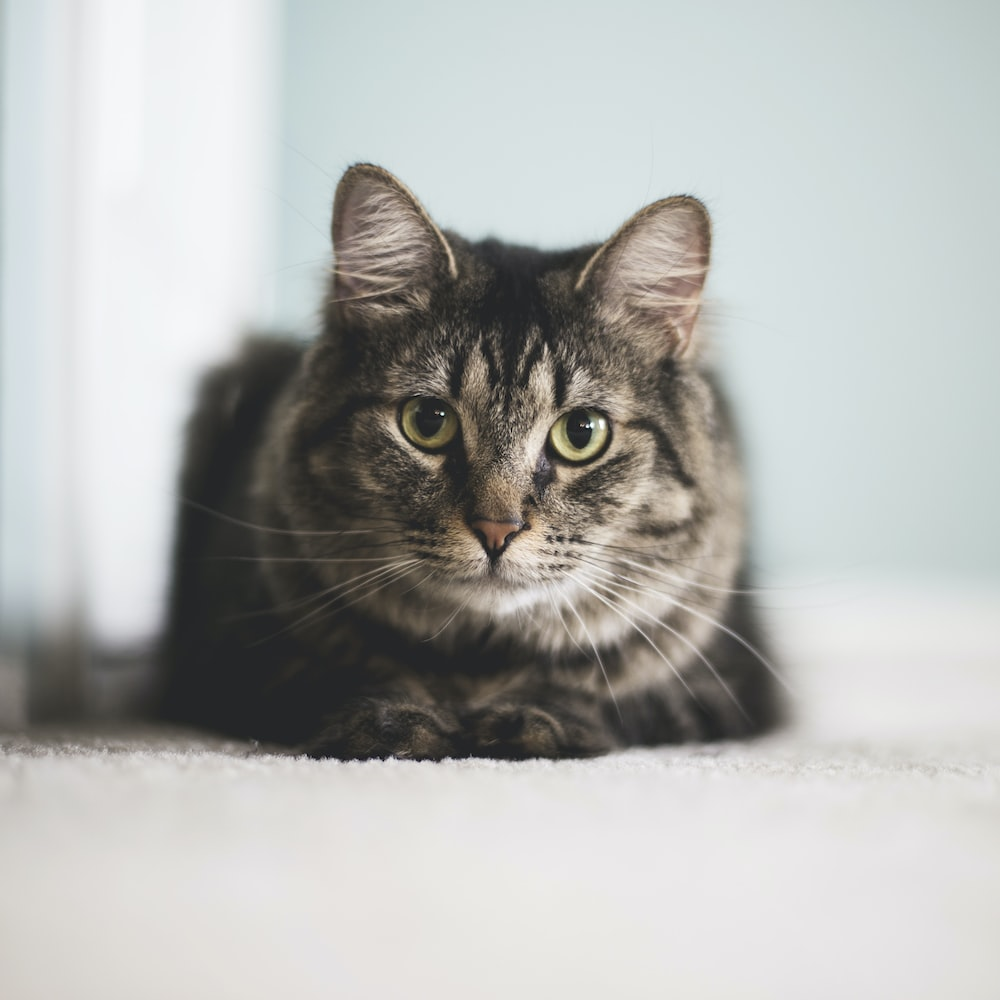
\includegraphics[width=2cm]{data/cat.jpeg}
	% 		};

	% 		\node[draw=black, fill=nodefill, circle, inner sep=4pt] (n00) at (-1.5, -3) {};
	% 		\node[draw=black, fill=nodefill, circle, inner sep=4pt] (n01) at (-1.5, -3.5) {};
	% 		\node[draw=black, fill=nodefill, circle, inner sep=4pt] (n02) at (-1.5, -4) {};
	% 		\node[draw=black, fill=nodefill, circle, inner sep=4pt] (n03) at (-1.5, -4.5) {};
	% 		\node[draw=black, fill=nodefill, circle, inner sep=4pt] (n04) at (-1.5, -5) {};

	% 		\node[draw=black, fill=nodefill, circle, inner sep=4pt] (n10) at (-0.75, -3.25) {};
	% 		\node[draw=black, fill=nodefill, circle, inner sep=4pt] (n11) at (-0.75, -3.75) {};
	% 		\node[draw=black, fill=nodefill, circle, inner sep=4pt] (n12) at (-0.75, -4.25) {};
	% 		\node[draw=black, fill=nodefill, circle, inner sep=4pt] (n13) at (-0.75, -4.75) {};

	% 		\node[draw=black, fill=nodefill, circle, inner sep=4pt] (n20) at (0, -3.5) {};
	% 		\node[draw=black, fill=nodefill, circle, inner sep=4pt] (n21) at (0, -4) {};
	% 		\node[draw=black, fill=nodefill, circle, inner sep=4pt] (n22) at (0, -4.5) {};

	% 		\node[draw=black, fill=nodefill, circle, inner sep=4pt] (n30) at (0.75, -3.75) {};
	% 		\node[draw=black, fill=nodefill, circle, inner sep=4pt] (n31) at (0.75, -4.25) {};

	% 		\node[draw=black, fill=nodefill, circle, inner sep=4pt] (n40) at (1.5, -4) {};

	% 		\draw[-Latex] (in.east) -- (n00);
	% 		\draw[-Latex] (in.east) -- (n01);
	% 		\draw[-Latex] (in.east) -- (n02);
	% 		\draw[-Latex] (in.east) -- (n03);
	% 		\draw[-Latex] (in.east) -- (n04);

	% 		\draw[] (n00) -- (n10);
	% 		\draw[] (n00) -- (n11);
	% 		\draw[] (n00) -- (n12);
	% 		\draw[] (n00) -- (n13);
	% 		\draw[] (n01) -- (n10);
	% 		\draw[] (n01) -- (n11);
	% 		\draw[] (n01) -- (n12);
	% 		\draw[] (n01) -- (n13);
	% 		\draw[] (n02) -- (n10);
	% 		\draw[] (n02) -- (n11);
	% 		\draw[] (n02) -- (n12);
	% 		\draw[] (n02) -- (n13);
	% 		\draw[] (n03) -- (n10);
	% 		\draw[] (n03) -- (n11);
	% 		\draw[] (n03) -- (n12);
	% 		\draw[] (n03) -- (n13);
	% 		\draw[] (n04) -- (n10);
	% 		\draw[] (n04) -- (n11);
	% 		\draw[] (n04) -- (n12);
	% 		\draw[] (n04) -- (n13);

	% 		\draw[] (n10) -- (n20);
	% 		\draw[] (n10) -- (n21);
	% 		\draw[] (n10) -- (n22);
	% 		\draw[] (n11) -- (n20);
	% 		\draw[] (n11) -- (n21);
	% 		\draw[] (n11) -- (n22);
	% 		\draw[] (n12) -- (n20);
	% 		\draw[] (n12) -- (n21);
	% 		\draw[] (n12) -- (n22);
	% 		\draw[] (n13) -- (n20);
	% 		\draw[] (n13) -- (n21);
	% 		\draw[] (n13) -- (n22);

	% 		\draw[] (n20) -- (n30);
	% 		\draw[] (n20) -- (n31);
	% 		\draw[] (n21) -- (n30);
	% 		\draw[] (n21) -- (n31);
	% 		\draw[] (n22) -- (n30);
	% 		\draw[] (n22) -- (n31);

	% 		\draw[] (n30) -- (n40);
	% 		\draw[] (n31) -- (n40);

	% 		\node[] at (-5, -3) {};
	% 		\node[] at (3.75, -6.2) {};
	% 	\end{tikzpicture}
	% \end{frame}

	% \begin{frame}{Decision making: Learning} % Prediction
	% 	\centering
	% 	\begin{tikzpicture}
	% 		\node[draw=black, inner sep=0pt, label=below:cat] (in) at (-4, -4) {
	% 			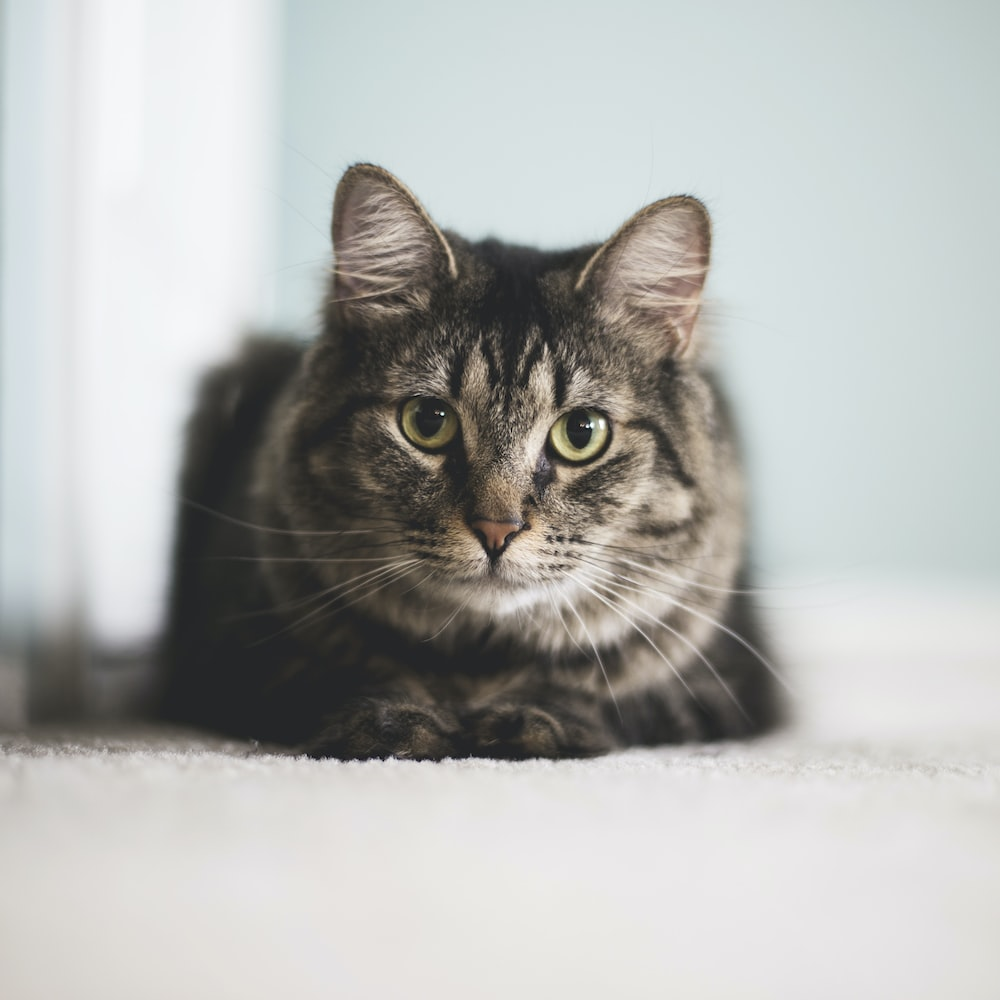
\includegraphics[width=2cm]{data/cat.jpeg}
	% 		};

	% 		\node[draw=black, fill=nodefill, circle, inner sep=4pt] (n00) at (-1.5, -3) {};
	% 		\node[draw=black, fill=nodefill, circle, inner sep=4pt] (n01) at (-1.5, -3.5) {};
	% 		\node[draw=black, fill=nodefill, circle, inner sep=4pt] (n02) at (-1.5, -4) {};
	% 		\node[draw=black, fill=nodefill, circle, inner sep=4pt] (n03) at (-1.5, -4.5) {};
	% 		\node[draw=black, fill=nodefill, circle, inner sep=4pt] (n04) at (-1.5, -5) {};

	% 		\node[draw=black, fill=nodefill, circle, inner sep=4pt] (n10) at (-0.75, -3.25) {};
	% 		\node[draw=black, fill=nodefill, circle, inner sep=4pt] (n11) at (-0.75, -3.75) {};
	% 		\node[draw=black, fill=nodefill, circle, inner sep=4pt] (n12) at (-0.75, -4.25) {};
	% 		\node[draw=black, fill=nodefill, circle, inner sep=4pt] (n13) at (-0.75, -4.75) {};

	% 		\node[draw=black, fill=nodefill, circle, inner sep=4pt] (n20) at (0, -3.5) {};
	% 		\node[draw=black, fill=nodefill, circle, inner sep=4pt] (n21) at (0, -4) {};
	% 		\node[draw=black, fill=nodefill, circle, inner sep=4pt] (n22) at (0, -4.5) {};

	% 		\node[draw=black, fill=nodefill, circle, inner sep=4pt] (n30) at (0.75, -3.75) {};
	% 		\node[draw=black, fill=nodefill, circle, inner sep=4pt] (n31) at (0.75, -4.25) {};

	% 		\node[draw=black, fill=nodefill, circle, inner sep=4pt] (n40) at (1.5, -4) {};

	% 		\node[] (out) at (3, -4) {dog};

	% 		\draw[-Latex] (in.east) -- (n00);
	% 		\draw[-Latex] (in.east) -- (n01);
	% 		\draw[-Latex] (in.east) -- (n02);
	% 		\draw[-Latex] (in.east) -- (n03);
	% 		\draw[-Latex] (in.east) -- (n04);

	% 		\draw[] (n00) -- (n10);
	% 		\draw[] (n00) -- (n11);
	% 		\draw[] (n00) -- (n12);
	% 		\draw[] (n00) -- (n13);
	% 		\draw[] (n01) -- (n10);
	% 		\draw[] (n01) -- (n11);
	% 		\draw[] (n01) -- (n12);
	% 		\draw[] (n01) -- (n13);
	% 		\draw[] (n02) -- (n10);
	% 		\draw[] (n02) -- (n11);
	% 		\draw[] (n02) -- (n12);
	% 		\draw[] (n02) -- (n13);
	% 		\draw[] (n03) -- (n10);
	% 		\draw[] (n03) -- (n11);
	% 		\draw[] (n03) -- (n12);
	% 		\draw[] (n03) -- (n13);
	% 		\draw[] (n04) -- (n10);
	% 		\draw[] (n04) -- (n11);
	% 		\draw[] (n04) -- (n12);
	% 		\draw[] (n04) -- (n13);

	% 		\draw[] (n10) -- (n20);
	% 		\draw[] (n10) -- (n21);
	% 		\draw[] (n10) -- (n22);
	% 		\draw[] (n11) -- (n20);
	% 		\draw[] (n11) -- (n21);
	% 		\draw[] (n11) -- (n22);
	% 		\draw[] (n12) -- (n20);
	% 		\draw[] (n12) -- (n21);
	% 		\draw[] (n12) -- (n22);
	% 		\draw[] (n13) -- (n20);
	% 		\draw[] (n13) -- (n21);
	% 		\draw[] (n13) -- (n22);

	% 		\draw[] (n20) -- (n30);
	% 		\draw[] (n20) -- (n31);
	% 		\draw[] (n21) -- (n30);
	% 		\draw[] (n21) -- (n31);
	% 		\draw[] (n22) -- (n30);
	% 		\draw[] (n22) -- (n31);

	% 		\draw[] (n30) -- (n40);
	% 		\draw[] (n31) -- (n40);

	% 		\draw[-Latex] (n40) -- (out);

	% 		\node[] at (-5, -3) {};
	% 		\node[] at (3.75, -6.2) {};
	% 	\end{tikzpicture}
	% \end{frame}


	% \begin{frame}{Decision making: Learning} % Loss
	% 	\centering
	% 	\begin{tikzpicture}
	% 		\node[draw=black, inner sep=0pt, label=below:cat] (in) at (-4, -4) {
	% 			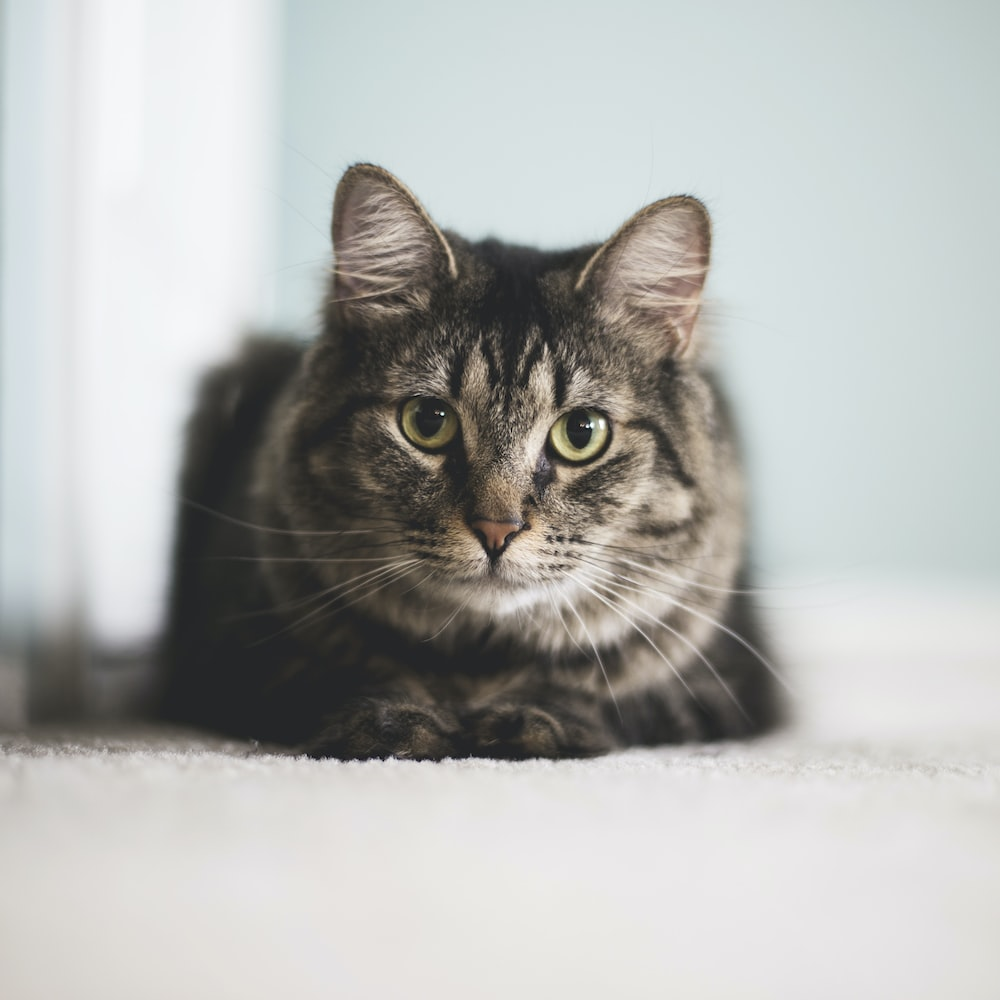
\includegraphics[width=2cm]{data/cat.jpeg}
	% 		};

	% 		\node[draw=black, fill=nodefill, circle, inner sep=4pt] (n00) at (-1.5, -3) {};
	% 		\node[draw=black, fill=nodefill, circle, inner sep=4pt] (n01) at (-1.5, -3.5) {};
	% 		\node[draw=black, fill=nodefill, circle, inner sep=4pt] (n02) at (-1.5, -4) {};
	% 		\node[draw=black, fill=nodefill, circle, inner sep=4pt] (n03) at (-1.5, -4.5) {};
	% 		\node[draw=black, fill=nodefill, circle, inner sep=4pt] (n04) at (-1.5, -5) {};

	% 		\node[draw=black, fill=nodefill, circle, inner sep=4pt] (n10) at (-0.75, -3.25) {};
	% 		\node[draw=black, fill=nodefill, circle, inner sep=4pt] (n11) at (-0.75, -3.75) {};
	% 		\node[draw=black, fill=nodefill, circle, inner sep=4pt] (n12) at (-0.75, -4.25) {};
	% 		\node[draw=black, fill=nodefill, circle, inner sep=4pt] (n13) at (-0.75, -4.75) {};

	% 		\node[draw=black, fill=nodefill, circle, inner sep=4pt] (n20) at (0, -3.5) {};
	% 		\node[draw=black, fill=nodefill, circle, inner sep=4pt] (n21) at (0, -4) {};
	% 		\node[draw=black, fill=nodefill, circle, inner sep=4pt] (n22) at (0, -4.5) {};

	% 		\node[draw=black, fill=nodefill, circle, inner sep=4pt] (n30) at (0.75, -3.75) {};
	% 		\node[draw=black, fill=nodefill, circle, inner sep=4pt] (n31) at (0.75, -4.25) {};

	% 		\node[draw=black, fill=nodefill, circle, inner sep=4pt] (n40) at (1.5, -4) {};

	% 		\node[] (out) at (3, -4) {dog};

	% 		\draw[-Latex] (in.east) -- (n00);
	% 		\draw[-Latex] (in.east) -- (n01);
	% 		\draw[-Latex] (in.east) -- (n02);
	% 		\draw[-Latex] (in.east) -- (n03);
	% 		\draw[-Latex] (in.east) -- (n04);

	% 		\draw[] (n00) -- (n10);
	% 		\draw[] (n00) -- (n11);
	% 		\draw[] (n00) -- (n12);
	% 		\draw[] (n00) -- (n13);
	% 		\draw[] (n01) -- (n10);
	% 		\draw[] (n01) -- (n11);
	% 		\draw[] (n01) -- (n12);
	% 		\draw[] (n01) -- (n13);
	% 		\draw[] (n02) -- (n10);
	% 		\draw[] (n02) -- (n11);
	% 		\draw[] (n02) -- (n12);
	% 		\draw[] (n02) -- (n13);
	% 		\draw[] (n03) -- (n10);
	% 		\draw[] (n03) -- (n11);
	% 		\draw[] (n03) -- (n12);
	% 		\draw[] (n03) -- (n13);
	% 		\draw[] (n04) -- (n10);
	% 		\draw[] (n04) -- (n11);
	% 		\draw[] (n04) -- (n12);
	% 		\draw[] (n04) -- (n13);

	% 		\draw[] (n10) -- (n20);
	% 		\draw[] (n10) -- (n21);
	% 		\draw[] (n10) -- (n22);
	% 		\draw[] (n11) -- (n20);
	% 		\draw[] (n11) -- (n21);
	% 		\draw[] (n11) -- (n22);
	% 		\draw[] (n12) -- (n20);
	% 		\draw[] (n12) -- (n21);
	% 		\draw[] (n12) -- (n22);
	% 		\draw[] (n13) -- (n20);
	% 		\draw[] (n13) -- (n21);
	% 		\draw[] (n13) -- (n22);

	% 		\draw[] (n20) -- (n30);
	% 		\draw[] (n20) -- (n31);
	% 		\draw[] (n21) -- (n30);
	% 		\draw[] (n21) -- (n31);
	% 		\draw[] (n22) -- (n30);
	% 		\draw[] (n22) -- (n31);

	% 		\draw[] (n30) -- (n40);
	% 		\draw[] (n31) -- (n40);

	% 		\draw[-Latex] (n40) -- (out);
	% 		\node[draw=black, dotted, label=below:\small{loss}] (loss) at ($ (out.south) - (0, 1.3) $) {\textcolor{red}{dog $\neq$ cat}};

	% 		\draw[-Latex] (out) -- (loss);

	% 		\node[] at (-5, -3) {};
	% 		\node[] at (3.75, -6.2) {};
	% 	\end{tikzpicture}
	% \end{frame}

	% \begin{frame}{Decision making: Learning} % Update
	% 	\centering
	% 	\begin{tikzpicture}
	% 		\node[draw=black, inner sep=0pt, label=below:cat] (in) at (-4, -4) {
	% 			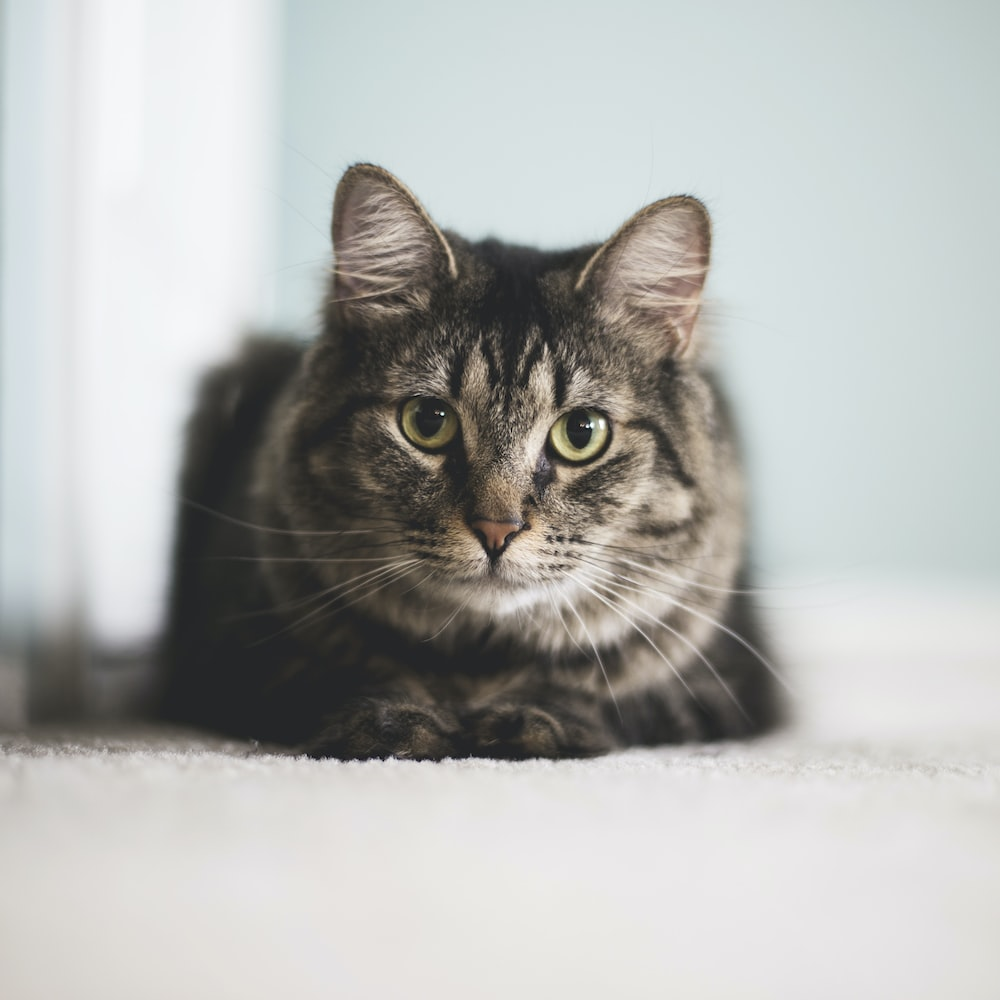
\includegraphics[width=2cm]{data/cat.jpeg}
	% 		};

	% 		\node[draw=black, fill=nodefill, circle, inner sep=4pt] (n00) at (-1.5, -3) {};
	% 		\node[draw=black, fill=nodefill, circle, inner sep=4pt] (n01) at (-1.5, -3.5) {};
	% 		\node[draw=black, fill=nodefill, circle, inner sep=4pt] (n02) at (-1.5, -4) {};
	% 		\node[draw=black, fill=nodefill, circle, inner sep=4pt] (n03) at (-1.5, -4.5) {};
	% 		\node[draw=black, fill=nodefill, circle, inner sep=4pt] (n04) at (-1.5, -5) {};

	% 		\node[draw=black, fill=nodefill, circle, inner sep=4pt] (n10) at (-0.75, -3.25) {};
	% 		\node[draw=black, fill=nodefill, circle, inner sep=4pt] (n11) at (-0.75, -3.75) {};
	% 		\node[draw=black, fill=nodefill, circle, inner sep=4pt] (n12) at (-0.75, -4.25) {};
	% 		\node[draw=black, fill=nodefill, circle, inner sep=4pt] (n13) at (-0.75, -4.75) {};

	% 		\node[draw=black, fill=nodefill, circle, inner sep=4pt] (n20) at (0, -3.5) {};
	% 		\node[draw=black, fill=nodefill, circle, inner sep=4pt] (n21) at (0, -4) {};
	% 		\node[draw=black, fill=nodefill, circle, inner sep=4pt] (n22) at (0, -4.5) {};

	% 		\node[draw=black, fill=nodefill, circle, inner sep=4pt] (n30) at (0.75, -3.75) {};
	% 		\node[draw=black, fill=nodefill, circle, inner sep=4pt] (n31) at (0.75, -4.25) {};

	% 		\node[draw=black, fill=nodefill, circle, inner sep=4pt] (n40) at (1.5, -4) {};

	% 		\node[] (out) at (3, -4) {dog};

	% 		\draw[-Latex] (in.east) -- (n00);
	% 		\draw[-Latex] (in.east) -- (n01);
	% 		\draw[-Latex] (in.east) -- (n02);
	% 		\draw[-Latex] (in.east) -- (n03);
	% 		\draw[-Latex] (in.east) -- (n04);

	% 		\draw[red] (n00) -- (n10);
	% 		\draw[red] (n00) -- (n11);
	% 		\draw[red] (n00) -- (n12);
	% 		\draw[red] (n00) -- (n13);
	% 		\draw[red] (n01) -- (n10);
	% 		\draw[red] (n01) -- (n11);
	% 		\draw[red] (n01) -- (n12);
	% 		\draw[red] (n01) -- (n13);
	% 		\draw[red] (n02) -- (n10);
	% 		\draw[red] (n02) -- (n11);
	% 		\draw[red] (n02) -- (n12);
	% 		\draw[red] (n02) -- (n13);
	% 		\draw[red] (n03) -- (n10);
	% 		\draw[red] (n03) -- (n11);
	% 		\draw[red] (n03) -- (n12);
	% 		\draw[red] (n03) -- (n13);
	% 		\draw[red] (n04) -- (n10);
	% 		\draw[red] (n04) -- (n11);
	% 		\draw[red] (n04) -- (n12);
	% 		\draw[red] (n04) -- (n13);

	% 		\draw[red] (n10) -- (n20);
	% 		\draw[red] (n10) -- (n21);
	% 		\draw[red] (n10) -- (n22);
	% 		\draw[red] (n11) -- (n20);
	% 		\draw[red] (n11) -- (n21);
	% 		\draw[red] (n11) -- (n22);
	% 		\draw[red] (n12) -- (n20);
	% 		\draw[red] (n12) -- (n21);
	% 		\draw[red] (n12) -- (n22);
	% 		\draw[red] (n13) -- (n20);
	% 		\draw[red] (n13) -- (n21);
	% 		\draw[red] (n13) -- (n22);

	% 		\draw[red] (n20) -- (n30);
	% 		\draw[red] (n20) -- (n31);
	% 		\draw[red] (n21) -- (n30);
	% 		\draw[red] (n21) -- (n31);
	% 		\draw[red] (n22) -- (n30);
	% 		\draw[red] (n22) -- (n31);

	% 		\draw[red] (n30) -- (n40);
	% 		\draw[red] (n31) -- (n40);

	% 		\draw[Latex-,red] (n40) -- (out);
	% 		\node[draw=black, dotted, label=below:\small{loss}] (loss) at ($ (out.south) - (0, 1.3) $) {\textcolor{red}{dog $\neq$ cat}};

	% 		\draw[Latex-,red] (out) -- (loss);

	% 		\node[] at (-5, -3) {};
	% 		\node[] at (3.75, -6.2) {};
	% 	\end{tikzpicture}
	% \end{frame}

	% \begin{frame}[t]{Decision making: Summary}
	% 	\vspace{2cm}
	% 	\textbf{How does a neural network make a decision?}\\
	% 	By looking for patterns in input data it has learned to recognize based on training to solve a specific task, represented by a loss function, using training data.
	% \end{frame}

	% \begin{frame}[t]{Decision making: Summary}
	% 	\vspace{2cm}
	% 	\textbf{How does a neural network make a decision?}\\
	% 	By looking for patterns in input data it has learned to recognize based on training to solve a \textcolor{red}{\textit{specific} task}, represented by a \textcolor{red}{loss function}, using \textcolor{red}{training data}.
	% 	\begin{itemize}
	% 		\item[\textcolor{green}+] The model will get very good at this task.
	% 		\item[\textcolor{red}-] The model will not take considerations beyond this task, e.g. emotions, justice, morality.
	% 		\item[\textcolor{green}+] The model apply patterns from its training data that were sufficient to solve the task there.
	% 		\item[\textcolor{red}-] There is no guarantee these patterns are sufficient in new data.
	% 		\item[\textcolor{red}-] No guarantee these patterns are ones we want to use (e.g. bias).
	% 	\end{itemize}
	% \end{frame}

	% \begin{frame}{Decision making: Group work}
	% 	We are dealing with an automatic systems in a bank that decide which clients are allowed a loan.
	% 	\begin{itemize}
	% 		\item In the center of the system is a machine learning model that predicts the probability of a client defaulting. This model is a fully deterministic mathematical formula that takes some numbers in a give a number out. The model was trained on training data from the bank.
	% 		\item Around the neural network is a software system which the user interacts with. After the user has input data, the system gives it to the neural network. If the neural network predicts a probability higher than 20\%, the loan is declined. The threshold of 20\% was implemented by a programmer, informed on the basis of a business analyst.
	% 	\end{itemize}
	% 	A client gets his loan declined. Who or what made the decision?
	% \end{frame}

	% \begin{frame}[t]{Decision making: Generalization} % Train/test
	% 	\centering
	% 	\textbf{There is no guarantee the patterns the model has learned are sufficient in new data.}
	% 	\begin{itemize}
	% 		\item "AI that is based on datasets cannot go beyond what is in the data." - Reasoning, Judging, Deciding: The Science of Thinking, Ch. 15
	% 	\end{itemize}
	% 	\vspace{0.5cm}
	% \end{frame}

	% \begin{frame}[t]{Decision making: Generalization} % Inference
	% 	\centering
	% 	\textbf{There is no guarantee the patterns the model has learned are sufficient in new data.}
	% 	\begin{itemize}
	% 		\item "AI that is based on datasets cannot go beyond what is in the data." - Reasoning, Judging, Deciding: The Science of Thinking, Ch. 15
	% 		\item While machine learning models are trained on a specific dataset (commonly referred to as the training set), they are almost always evaluated on a different dataset (called the test set).
	% 	\end{itemize}
	% \end{frame}

	% \begin{frame}[t]{Decision making: Generalization} % Inference
	% 	\centering
	% 	\textbf{There is no guarantee the patterns the model has learned are sufficient in new data.}
	% 	\begin{itemize}
	% 		\item "AI that is based on datasets cannot go beyond what is in the data." -Reasoning, Judging, Deciding: The Science of Thinking, Ch. 15
	% 		\item While machine learning models are trained on a specific dataset (commonly referred to as the training set), they are almost always evaluated on a different dataset (called the test set).
	% 	\end{itemize}
	% 	\vspace{0.5cm}
	% 	\begin{tikzpicture}
	% 		\begin{axis}[
	% 			xlabel={Apartment size (sq. m.)},
	% 			ylabel={Apartment value (NOK)},
	% 			width=8cm,
	% 			height=6cm,
	% 			ymax=6,
	% 			ymin=-2,
	% 			xmin=0,
	% 			xmax=3,
	% 			ticks=none,
	% 			axis x line=bottom,
	% 			axis y line=left
	% 		]

	% 		\addplot[blue!60, only marks] coordinates {
	% 			(1, 2)
	% 			(2, 4)
	% 		};

	% 		\end{axis}
	% 	\end{tikzpicture}
	% \end{frame}

	% \begin{frame}[t]{Decision making: Generalization} % Interpolation
	% 	\centering
	% 	\textbf{There is no guarantee the patterns the model has learned are sufficient in new data.}
	% 	\begin{itemize}
	% 		\item "AI that is based on datasets cannot go beyond what is in the data." - Reasoning, Judging, Deciding: The Science of Thinking, Ch. 15
	% 		\item While machine learning models are trained on a specific dataset (commonly referred to as the training set), they are almost always evaluated on a different dataset (called the test set).
	% 	\end{itemize}
	% 	\vspace{0.5cm}
	% 	\begin{tikzpicture}
	% 		\begin{axis}[
	% 			xlabel={Apartment size (sq. m.)},
	% 			ylabel={Apartment value (NOK)},
	% 			width=8cm,
	% 			height=6cm,
	% 			ymax=6,
	% 			ymin=-2,
	% 			xmin=0,
	% 			xmax=3,
	% 			ticks=none,
	% 			axis x line=bottom,
	% 			axis y line=left
	% 		]

	% 		\addplot[blue!60, only marks] coordinates {
	% 			(1, 2)
	% 			(2, 4)
	% 		};
	% 		\addplot[green!60, only marks] coordinates {
	% 			(1.5, 3)
	% 		};

	% 		\end{axis}
	% 	\end{tikzpicture}
	% \end{frame}

	% \begin{frame}[t]{Decision making: Generalization} % Extrapolation
	% 	\centering
	% 	\textbf{There is no guarantee the patterns the model has learned are sufficient in new data.}
	% 	\begin{itemize}
	% 		\item "AI that is based on datasets cannot go beyond what is in the data." - Reasoning, Judging, Deciding: The Science of Thinking, Ch. 15
	% 		\item While machine learning models are trained on a specific dataset (commonly referred to as the training set), they are almost always evaluated on a different dataset (called the test set).
	% 	\end{itemize}
	% 	\vspace{0.5cm}
	% 	\begin{tikzpicture}
	% 		\begin{axis}[
	% 			xlabel={Apartment size (sq. m.)},
	% 			ylabel={Apartment value (NOK)},
	% 			width=8cm,
	% 			height=6cm,
	% 			ymax=6,
	% 			ymin=-2,
	% 			xmin=0,
	% 			xmax=3,
	% 			ticks=none,
	% 			axis x line=bottom,
	% 			axis y line=left
	% 		]

	% 		\addplot[blue!60, only marks] coordinates {
	% 			(1, 2)
	% 			(2, 4)
	% 		};
	% 		\addplot[green!60, only marks] coordinates {
	% 			(1.5, 3)
	% 		};
	% 		\addplot[red!60, only marks] coordinates {
	% 			(0.5, 1)
	% 			(2.5, 5)
	% 		};

	% 		\end{axis}
	% 	\end{tikzpicture}
	% \end{frame}

	% \begin{frame}[t]{Decision making: Biases} % Plot
	% 	\textbf{No guarantee the patterns the models has learned are ones we want to use}
	% 	\begin{itemize}
	% 		\item The model can rely on variables we do not want to drive the predictions (age, gender, nationality) due to correlations in training data.
	% 		\item This can occur even when the model is not explicitly trained to use these variables.
	% 		\item Thus models perpetuate and potentially amplify societal biases occuring in its training data.
	% 	\end{itemize}
	% \end{frame}

	% \setbeamertemplate{footline}[compas]

	% \begin{frame}[t]{Decision making: Biases} % COMPAS
	% 	\textbf{No guarantee the patterns the models has learned are ones we want to use}
	% 	\begin{itemize}
	% 		\item The model can rely on variables we do not want to drive the predictions (age, gender, nationality) due to correlations in training data.
	% 		\item This can occur even when the model is not explicitly trained to use these variables.
	% 		\item Thus models perpetuate and potentially amplify societal biases occuring in its training data.
	% 	\end{itemize}
	% 	\textbf{Bias in criminal risk assessment (Dressel \& Farid, 2018)}
	% 	\begin{itemize}
	% 		\item Comparison of the ability of COMPAS, a commercial risk assessment software, and non-expert humans to predict re-arrest.
	% 	\end{itemize}
	% \end{frame}

	% \begin{frame}[t]{Decision making: Biases} % COMPAS: Plot
	% 	\textbf{No guarantee the patterns the models has learned are ones we want to use}
	% 	\begin{itemize}
	% 		\item The model can rely on variables we do not want to drive the predictions (age, gender, nationality) due to correlations in training data.
	% 		\item This can occur even when the model is not explicitly trained to use these variables.
	% 		\item Thus models perpetuate and potentially amplify societal biases occuring in its training data.
	% 	\end{itemize}
	% 	\textbf{Bias in criminal risk assessment (Dressel \& Farid, 2018)}
	% 	\begin{itemize}
	% 		\item Comparison of the ability of COMPAS, a commercial risk assessment software, and non-expert humans to predict re-arrest.
	% 	\end{itemize}
	% 	\centering
	% 	\begin{tikzpicture}
	% 		\node[inner sep=0pt, draw=black] {
	% 			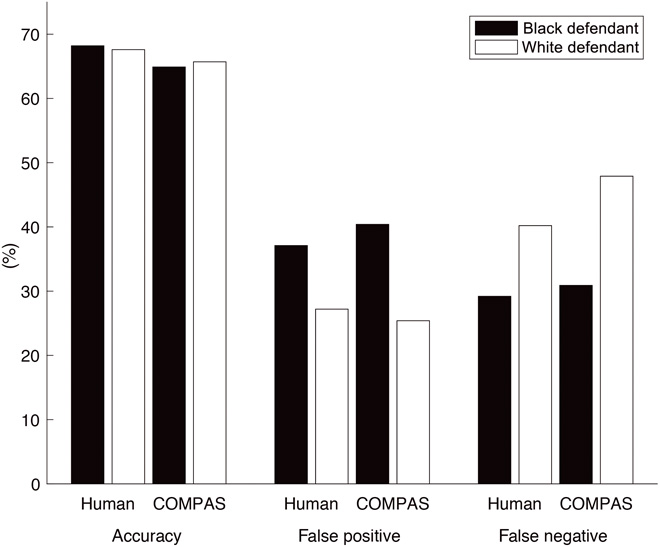
\includegraphics[width=3cm]{data/compas.jpeg}
	% 		};
	% 	\end{tikzpicture}
	% \end{frame}

	% \begin{frame}[t]{Decision making: Biases} % COMPAS: Bias
	% 	\textbf{No guarantee the patterns the models has learned are ones we want to use}
	% 	\begin{itemize}
	% 		\item The model can rely on variables we do not want to drive the predictions (age, gender, nationality) due to correlations in training data.
	% 		\item This can occur even when the model is not explicitly trained to use these variables.
	% 		\item Thus models perpetuate and potentially amplify societal biases occuring in its training data.
	% 	\end{itemize}
	% 	\textbf{Bias in criminal risk assessment (Dressel \& Farid, 2018)}
	% 	\begin{itemize}
	% 		\item Comparison of the ability of COMPAS, a commercial risk assessment software, and non-expert humans to predict re-arrest.
	% 		\item Both COMPAS and humans were biased against black offenders, even when race was not used in the data.
	% 	\end{itemize}
	% \end{frame}

	% \begin{frame}[t]{Decision making: Biases} % COMPAS: Accuracy
	% 	\textbf{No guarantee the patterns the models has learned are ones we want to use}
	% 	\begin{itemize}
	% 		\item The model can rely on variables we do not want to drive the predictions (age, gender, nationality) due to correlations in training data.
	% 		\item This can occur even when the model is not explicitly trained to use these variables.
	% 		\item Thus models perpetuate and potentially amplify societal biases occuring in its training data.
	% 	\end{itemize}
	% 	\textbf{Bias in criminal risk assessment (Dressel \& Farid, 2018)}
	% 	\begin{itemize}
	% 		\item Comparison of the ability of COMPAS, a commercial risk assessment software, and non-expert humans to predict re-arrest.
	% 		\item Both COMPAS and humans were biased against black offenders, even when race was not used in the data.
	% 		\item "it is valuable to ask whether we would put these decisions in the hands of random people ..., [which] appear to be indistinguishable."
	% 	\end{itemize}
	% \end{frame}

	% \setbeamertemplate{footline}[humanbias]

	% \begin{frame}[t]{Decision making: Biases} % COMPAS: Accuracy
	% 	\textbf{No guarantee the patterns the models has learned are ones we want to use}
	% 	\begin{itemize}
	% 		\item The model can rely on variables we do not want to drive the predictions (age, gender, nationality) due to correlations in training data.
	% 		\item This can occur even when the model is not explicitly trained to use these variables.
	% 		\item Thus models perpetuate and potentially amplify societal biases occuring in its training data.
	% 	\end{itemize}
	% 	\textbf{Bias in hiring (Bertrand \& Mullainathan, 2004)}
	% 	\begin{itemize}
	% 		\item Evaluation of bias in human decision making in help-wanted advertisements in the US.
	% 		\item "Applicants" were given very African American or European-sounding names.
	% 		\item European names received 50\% more callbacks for interviews.
	% 		\item Applicants from neighbourhoods considered higher class received more callbacks.
	% 		\item Employers listing themselves as an "Equal Opportunity Employer" were as biased as others.
	% 	\end{itemize}
	% \end{frame}

	% \setbeamertemplate{footline}[default]

	% \begin{frame}[t]{Decision making: Theory of mind}
	% 	\textbf{Does AI consider humans as thinking and feeling beings?}
	% 	\begin{itemize}
	% 		\item "... This is an instance of AI programs lacking true Theory of Mind capability." - Reasoning, Judging, Deciding: The Science of Thinking, Ch. 15
	% 		\item Theory of mind: The ability to "track others' unobservable mental states, such as their knowledge, intentions, beliefs, and desires." (Kosinski 2023)
	% 	\end{itemize}
	% \end{frame}

	% \setbeamertemplate{footline}[pedestrian]

	% \begin{frame}[t]{Decision making: Theory of mind}
	% 	\textbf{Does AI consider humans as thinking and feeling beings?}
	% 	\begin{itemize}
	% 		\item "... This is an instance of AI programs lacking true Theory of Mind capability." - Reasoning, Judging, Deciding: The Science of Thinking, Ch. 15
	% 		\item Theory of mind: The ability to "track others' unobservable mental states, such as their knowledge, intentions, beliefs, and desires." (Kosinski 2023)
	% 	\end{itemize}
	% 	\textbf{Pedestrian modelling in self-driving cars (Gulzar et al., 2021)}\\
	% 	\centering
	% 	\vspace{0.5cm}
	% 	\begin{tikzpicture}
	% 		\node[inner sep=0pt, draw=black] {
	% 			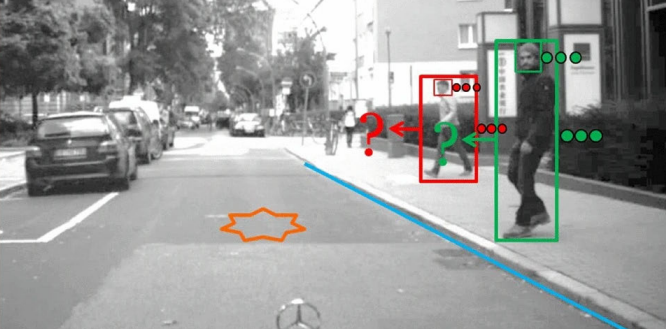
\includegraphics[width=8cm]{data/pedestrian.png}
	% 		};
	% 	\end{tikzpicture}
	% \end{frame}

	% \setbeamertemplate{footline}[theoryofmind]

	% \begin{frame}[t]{Decision making: Theory of mind}
	% 	\textbf{Does AI consider humans as thinking and feeling beings?}
	% 	\begin{itemize}
	% 		\item "... This is an instance of AI programs lacking true Theory of Mind capability." - Reasoning, Judging, Deciding: The Science of Thinking, Ch. 15
	% 		\item Theory of mind: The ability to "track others' unobservable mental states, such as their knowledge, intentions, beliefs, and desires." (Kosinski 2023)
	% 	\end{itemize}
	% 	\textbf{Theory of mind in ChatGPT (Kosinski, 2023)}\\
	% 	\centering
	% 	\vspace{0.5cm}
	% 	\begin{tikzpicture}
	% 		\node[inner sep=0pt, draw=black] {
	% 			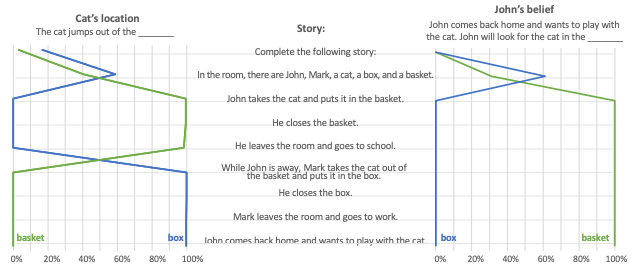
\includegraphics[width=9cm]{data/theory_of_mind.png}
	% 		};
	% 	\end{tikzpicture}
	% \end{frame}

	% \setbeamertemplate{footline}[default]

	% \begin{frame}[t]{Decision making: Creativity}
	% 	\textbf{Can AI create anything new?}
	% 	\begin{itemize}
	% 		\item "AI does not truly create" - Reasoning, Judging, Deciding: The Science of Thinking, Ch. 15
	% 		\item "AI lacks true imagination" - Reasoning, Judging, Deciding: The Science of Thinking, Ch. 15
	% 	\end{itemize}
	% \end{frame}

	% \begin{frame}[t]{Decision making: Creativity}
	% 	\textbf{Can AI create anything new?}
	% 	\begin{itemize}
	% 		\item "AI does not truly create" - Reasoning, Judging, Deciding: The Science of Thinking, Ch. 15
	% 		\item "AI lacks true imagination" - Reasoning, Judging, Deciding: The Science of Thinking, Ch. 15
	% 	\end{itemize}
	% 	\centering
	% 	\vspace{0.5cm}
	% 	\begin{tikzpicture}
	% 		\node[label=below:{Imagen: A cute corgi lives in a house made out of sushi}, inner sep=0pt, draw=black] {
	% 			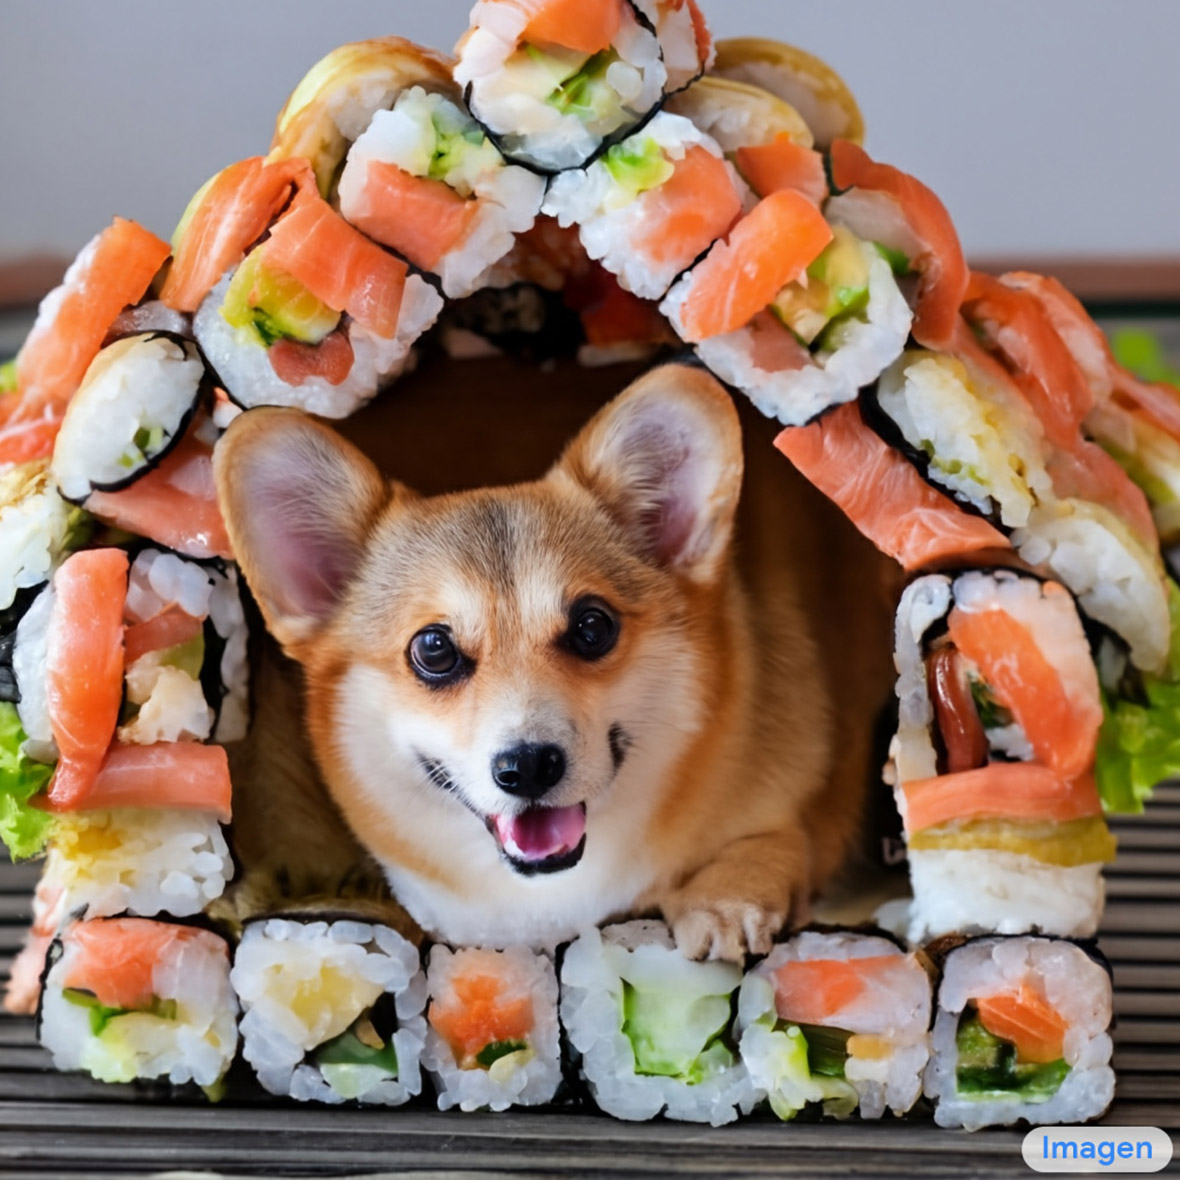
\includegraphics[width=5cm]{data/corgi.jpeg}
	% 		};
	% 	\end{tikzpicture}
	% \end{frame}

	% \setbeamertemplate{footline}[sparks]

	% \begin{frame}[t]{Decision making: Creativity}
	% 	\textbf{Can AI create anything new?}
	% 	\begin{itemize}
	% 		\item "AI does not truly create" - Reasoning, Judging, Deciding: The Science of Thinking, Ch. 15
	% 		\item "AI lacks true imagination" - Reasoning, Judging, Deciding: The Science of Thinking, Ch. 15
	% 	\end{itemize}
	% 	\textbf{GPT-4 displays creative mathematical thinking (Bubeck et al., 2023)}
	% 	\begin{itemize}
	% 		\item "The conversation reflects profound understanding of the undergraduate-level
	% 		mathematical concepts discussed, as well as a significant extent of creativity"
	% 	\end{itemize}
	% 	\vspace{0.5cm}
	% 	\centering
	% 	\begin{tikzpicture}
	% 		\node[inner sep=0pt, draw=black] {
	% 			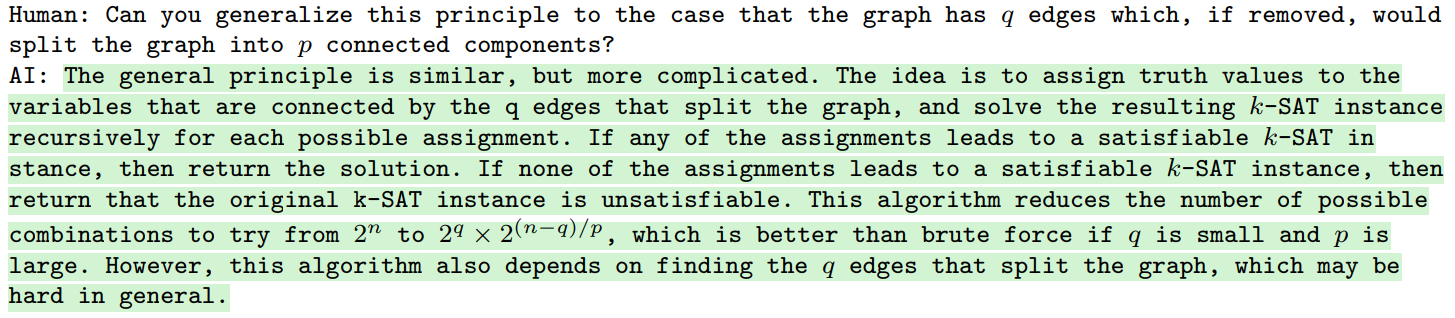
\includegraphics[width=8cm]{data/ksat}
	% 		};
	% 	\end{tikzpicture}
	% \end{frame}

	% \setbeamertemplate{footline}[creativity]

	% \begin{frame}[t]{Decision making: Creativity}
	% 	\textbf{Can AI create anything new?}
	% 	\begin{itemize}
	% 		\item "AI does not truly create" - Reasoning, Judging, Deciding: The Science of Thinking, Ch. 15
	% 		\item "AI lacks true imagination" - Reasoning, Judging, Deciding: The Science of Thinking, Ch. 15
	% 	\end{itemize}
	% 	\textbf{ChatGPTs creative prowess impresses Twitter (Taecharungroj, 2023)}
	% 	\begin{itemize}
	% 		\item "One of the most prominent features of ChatGPT is its ability
	% 		to generate creative writing. Twitter users have shared examples
	% 		of poems, rap songs, and made-up stories that ChatGPT has written"
	% 	\end{itemize}
	% 	\vspace{0.3cm}
	% 	\centering
	% 	\begin{tikzpicture}
	% 		\node[inner sep=0pt, draw=black] {
	% 			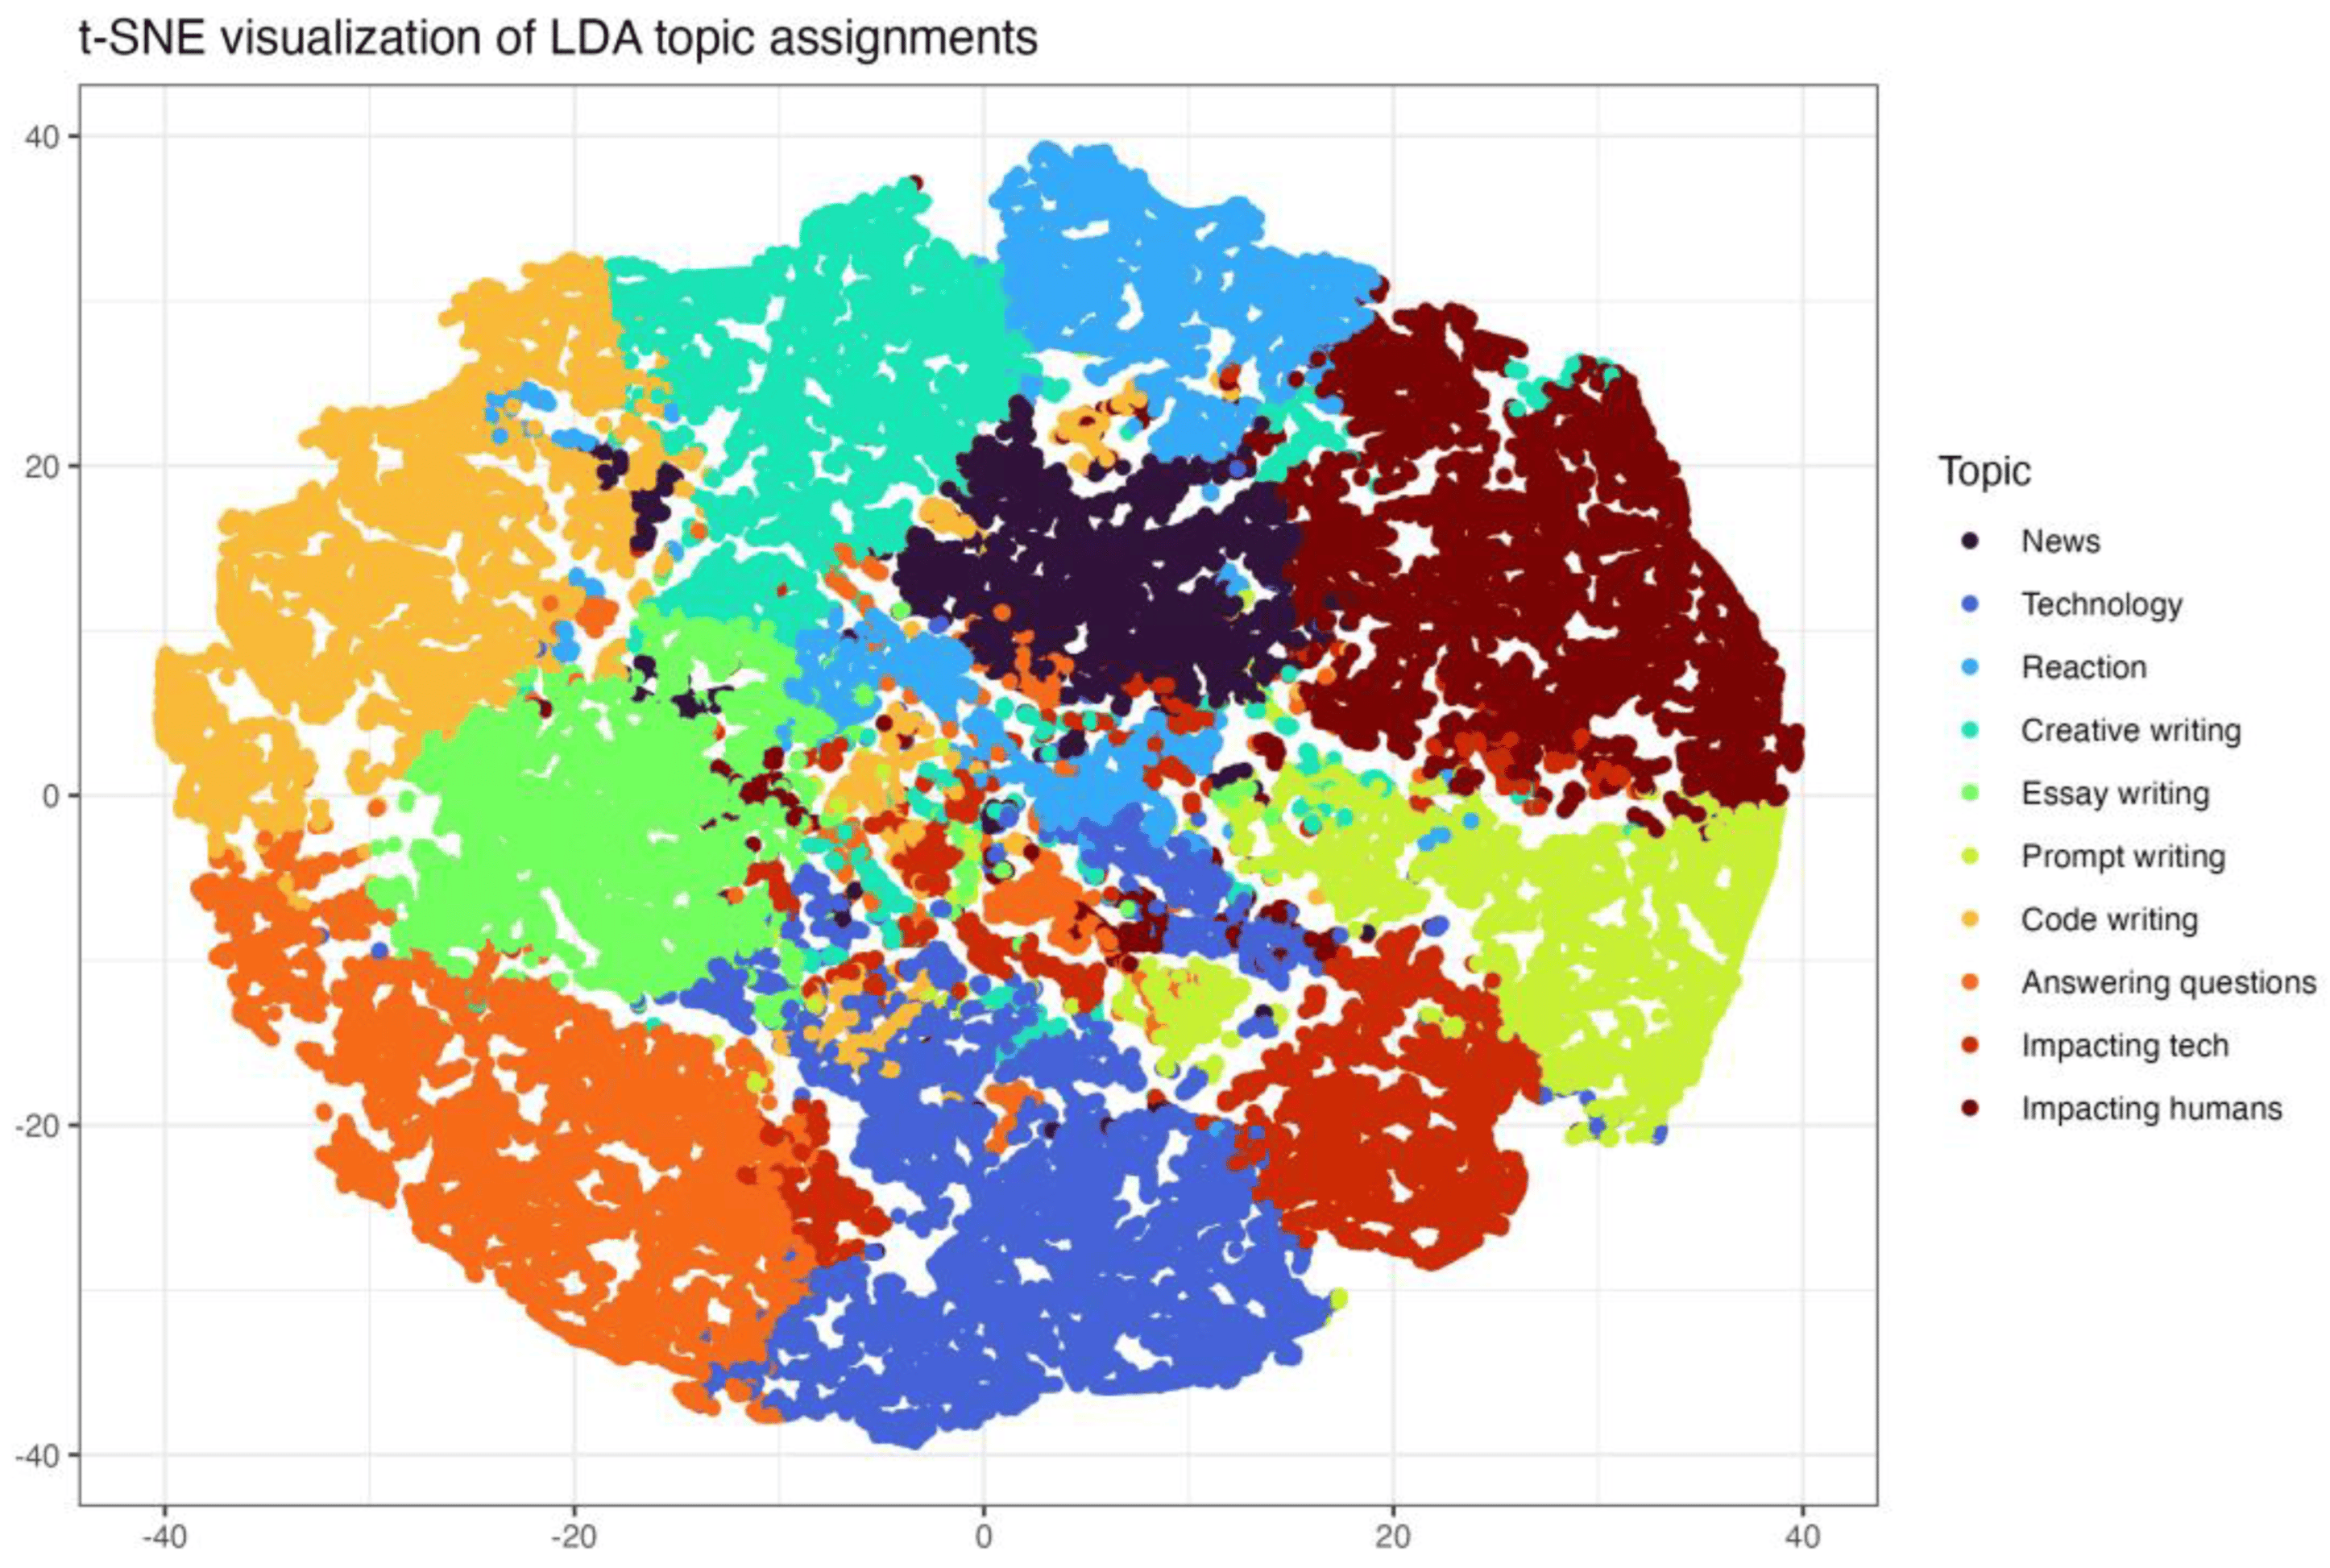
\includegraphics[width=5cm]{data/creativity.png}
	% 		};
	% 	\end{tikzpicture}
	% \end{frame}

	% \setbeamertemplate{footline}[default]

	% \begin{frame}{Decision making: Wisdom}
	% 	\textbf{Are AIs wise?}
	% 	\begin{itemize}
	% 		\item "... the expertise in the domain of fundamental life pragmatics, such as life planning or life review. It requires a rich factual knowledge about life matters, rich procedural knowledge about life problems, knowledge of different life contexts and values or priorities, and knowledge about the unpredictability of life." - easoning, Judging, Deciding: The Science of Thinking, Ch. 15 (adopted from Birren and Svensson, attributed to Baltes and Smith)
	% 		\item Current AI relies on correlations in data, not causal understanding.
	% 		\item Lacks commonsense understanding.
	% 		\item Unimodal (e.g. relies only on text), little opportunity to interact with the world.
	% 		\item \textbf{Little introspection towards its own limits or uncertainties.}
	% 	\end{itemize}
	% \end{frame}

	% \begin{frame}{Decision making: Summary}
	% 	\textbf{How does AI make decisions?}
	% 	\begin{itemize}
	% 		\item Learns to solve a \textit{very} specific problem.
	% 		\item Relies on correlations in training data.
	% 	\end{itemize}
	% 	\textbf{What can we expect from the decision made by AI?}
	% 	\begin{itemize}
	% 		\item Usually very good at the task it was trained for.
	% 		\item Lacks moral judgement, empathy and sense of justice.
	% 		\item Dangerous to rely on decisions based on input data that is out-of-distribution (extrapolation).
	% 		\item Potentially biased (but so are humans).
	% 		\item Uncertain whether they can imagine other actors with their own goals and desires.
	% 		\item Uncertain whether they can create anything new.
	% 		\item Lacks wisdom, a fundamental understanding of the world, and common sense.
	% 		\item \textbf{Reliable and objective (in one sense of the word)}
	% 	\end{itemize}
	% \end{frame}

	% \section{Decision support}

	% \begin{frame}[t]{Decision support: Content personalization}
	% 	\textbf{Helping users decide what to listen to}
	% 	\vspace{0.3cm}
	% 	\begin{center}
	% 		\begin{tikzpicture}
	% 			\node[] {
	% 				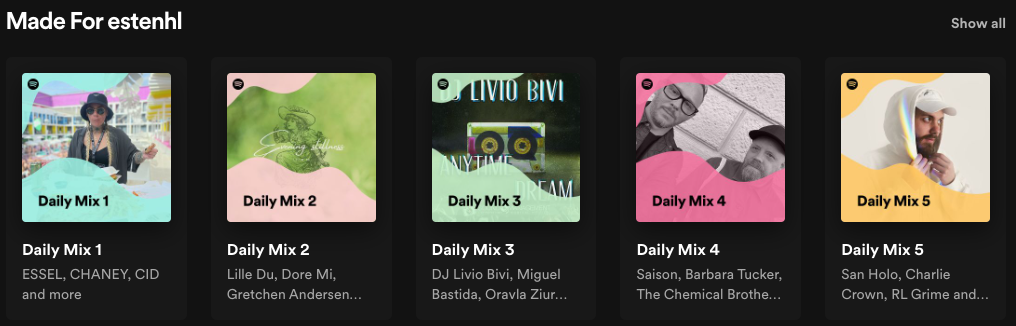
\includegraphics[width=9cm]{data/spotify.png}
	% 			};
	% 		\end{tikzpicture}
	% 	\end{center}
	% \end{frame}

	% \begin{frame}[t]{Decision support: Content personalization}
	% 	\textbf{Helping users decide what to listen to}
	% 	\vspace{0.3cm}
	% 	\begin{center}
	% 		\begin{tikzpicture}
	% 			\node[] {
	% 				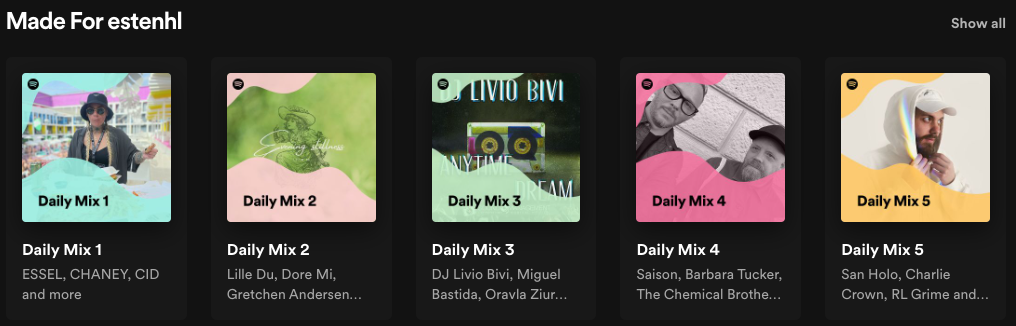
\includegraphics[width=9cm]{data/spotify.png}
	% 			};
	% 		\end{tikzpicture}
	% 	\end{center}
	% 	\vspace{0.3cm}
	% 	\begin{itemize}
	% 		\item Recommends content to users based on their history.
	% 		\item Has been around for a long time.
	% 		\item Extremely intricate trade-offs between exploitation, showing users what they like, and exploration, showing users new content.
	% 		\item \textbf{Based around recommendation, not clear cut decisions.}
	% 		\item Can potentially lead to feedback loops?
	% 	\end{itemize}
	% \end{frame}

	% \setbeamertemplate{footline}[vg]

	% \begin{frame}[t]{Decision support: Fracture detection}
	% 	\textbf{Helping doctors detect fractures in X-rays}\\
	% 	\begin{itemize}
	% 		\item Bærum sykehus is the first norwegian hospital to implement an AI powered decision support system into the clinic.
	% 		\item Helps alleviate a 12.5\% year-on-year increase in the prevalence of fractures.
	% 		\item 60\% to 70\% of all X-rays are normal, but still need to be reviewed by a radiologist.
	% 	\end{itemize}
	% 	\vspace{0.5cm}
	% 	\centering
	% 	\begin{tikzpicture}
	% 		\node[inner sep=0pt, draw=black] {
	% 			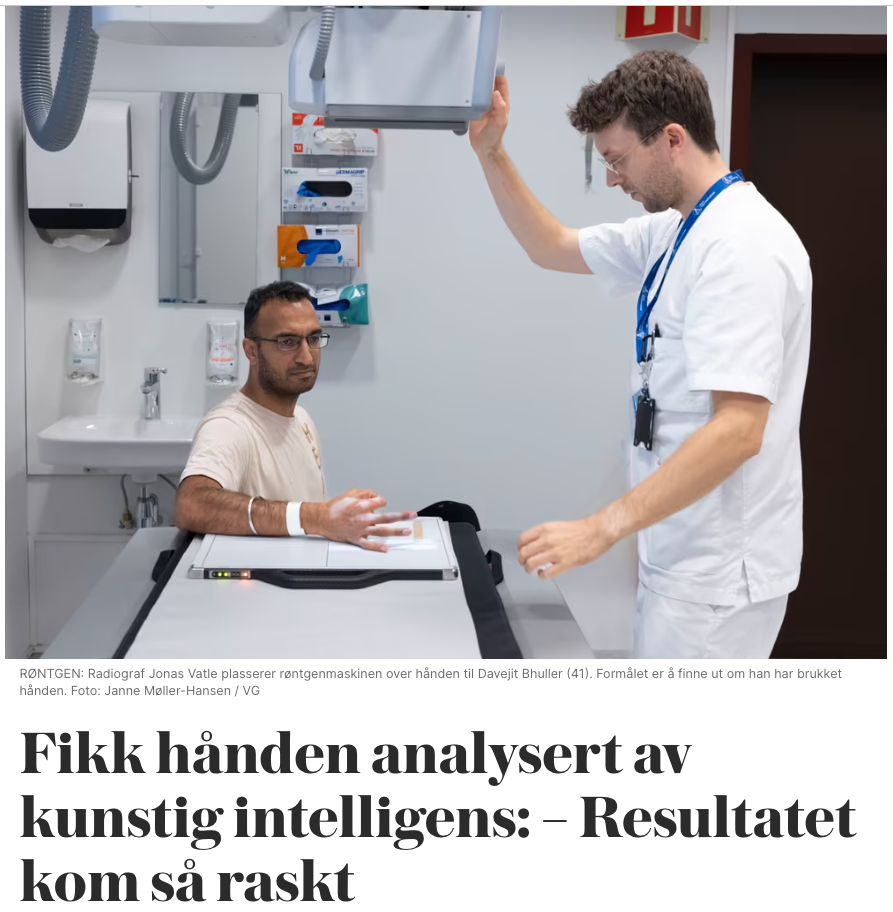
\includegraphics[width=4.5cm]{data/vg.png}
	% 		};
	% 	\end{tikzpicture}
	% \end{frame}

	% \setbeamertemplate{footline}[boneview]

	% \begin{frame}[t]{Decision support: Fracture detection}
	% 	\textbf{Helping doctors detect fractures in X-rays}\\
	% 	\begin{itemize}
	% 		\item Bærum sykehus is the first norwegian hospital to implement an AI powered decision support system into the clinic.
	% 		\item Helps alleviate a 12.5\% year-on-year increase in the prevalence of fractures.
	% 		\item 60\% to 70\% of all X-rays are normal, but still need to be reviewed by a radiologist.
	% 	\end{itemize}
	% 	\textbf{Assessing the efficacy of AI in fracture detection (Guermazi et al., 2022)}\\
	% 	\vspace{0.5cm}
	% 	\centering
	% 	\begin{tikzpicture}
	% 		\node[inner sep=0pt, draw=black] {
	% 			\includegraphics[width=3.5cm]{data/boneview.png}
	% 		};
	% 	\end{tikzpicture}
	% \end{frame}

	% \begin{frame}[t]{Decision support: Fracture detection}
	% 	\textbf{Helping doctors detect fractures in X-rays}\\
	% 	\begin{itemize}
	% 		\item Bærum sykehus is the first norwegian hospital to implement an AI powered decision support system into the clinic.
	% 		\item Helps alleviate a 12.5\% year-on-year increase in the prevalence of fractures.
	% 		\item 60\% to 70\% of all X-rays are normal, but still need to be reviewed by a radiologist.
	% 	\end{itemize}
	% 	\textbf{Assessing the efficacy of AI in fracture detection (Guermazi et al., 2022)}\\
	% 	\begin{itemize}
	% 		\item AI assistant on its own achieved an area under the receiver operating characteristic curve of 0.97.
	% 		\item Radiologist in conjunction with the AI assistant achieved a 10.4\% increase in sensitivity (64.8\% to 75.2\%), and an increase in specificity (90.6\% vs 95.6\%).
	% 		\item \textbf{Assistance from the AI reduced average reading time with 6.3 seconds}.
	% 	\end{itemize}
	% \end{frame}

	% \setbeamertemplate{footline}[covid]

	% \begin{frame}[t]{Decision support: COVID-19 severity}
	% 	\textbf{Helping doctors decide the severity of COVID-19 cases (Wysocki et al., 2023)}\\
	% 	\begin{itemize}
	% 		\item 23 healthcare professionals tasked to assess the severity of COVID-19 in ten patients using the COVID-19 Risk in ONcology Evaluation Tool (CORONET) tool.
	% 	\end{itemize}
	% 	\vspace{0.5cm}
	% 	\centering
	% 	\begin{tikzpicture}
	% 		\node[inner sep=0pt, draw=black] {
	% 			\includegraphics[width=9cm]{data/covid.png}
	% 		};
	% 	\end{tikzpicture}
	% \end{frame}

	% \begin{frame}[t]{Decision support: COVID-19 severity}
	% 	\textbf{Helping doctors decide the severity of COVID-19 cases (Wysocki et al., 2023)}\\
	% 	\begin{itemize}
	% 		\item 23 healthcare professionals tasked to assess the severity of COVID-19 in ten patients using the COVID-19 Risk in ONcology Evaluation Tool (CORONET) tool.
	% 		\item Asked about their experience using the tool.
	% 	\end{itemize}
	% 	\vspace{0.5cm}
	% 	\centering
	% 	\begin{tikzpicture}
	% 		\node[inner sep=0pt, draw=black] at (0, 0) {
	% 			\includegraphics[width=9cm]{data/questionnaire.png}
	% 		};
	% 	\end{tikzpicture}
	% \end{frame}

	% \begin{frame}[t]{Decision support: COVID-19 severity} % Uncertainty
	% 	\textbf{Helping doctors decide the severity of COVID-19 cases (Wysocki et al., 2023)}\\
	% 	\begin{itemize}
	% 		\item 23 healthcare professionals tasked to assess the severity of COVID-19 in ten patients using the COVID-19 Risk in ONcology Evaluation Tool (CORONET) tool.
	% 		\item Questioned about their experience using the tool.
	% 	\end{itemize}
	% 	\vspace{0.5cm}
	% 	\centering
	% 	\begin{tikzpicture}
	% 		\node[inner sep=0pt, draw=black] at (0, 0) {
	% 			\includegraphics[width=9cm]{data/questionnaire.png}
	% 		};
	% 		\node[draw=red, minimum width=6.2cm, minimum height=0.5cm, thick] at (-1.23, -0.85) {};
	% 	\end{tikzpicture}
	% \end{frame}

	% \begin{frame}[t]{Decision support: COVID-19 severity} % Uncertainty
	% 	\textbf{Helping doctors decide the severity of COVID-19 cases (Wysocki et al., 2023)}\\
	% 	\begin{itemize}
	% 		\item 23 healthcare professionals tasked to assess the severity of COVID-19 in ten patients using the COVID-19 Risk in ONcology Evaluation Tool (CORONET) tool.
	% 		\item Questioned about their experience using the tool.
	% 	\end{itemize}
	% 	\vspace{0.5cm}
	% 	\centering
	% 	\begin{tikzpicture}
	% 		\node[inner sep=0pt, draw=black] at (0, 0) {
	% 			\includegraphics[width=9cm]{data/questionnaire.png}
	% 		};
	% 		\node[draw=red, minimum width=6.3cm, minimum height=1cm, thick] at (-1.3, -0.1) {};
	% 	\end{tikzpicture}
	% \end{frame}

	% \setbeamertemplate{footline}[default]

	% \begin{frame}{Decision support: Black boxes} % Schematic
	% 	\begin{tikzpicture}
	% 		\node[draw=black, dashed] (in) at (-4, -0.75) {Laboratory report};

	% 		\node[draw=black, fill=background] (n00) at (0, 0) {
	% 			gram stain = gramneg
	% 		};
	% 		\node[draw=black, fill=background] (n01) at (0, -0.75) {
	% 			morphology = rod
	% 		};
	% 		\node[draw=black, fill=background] (n02) at (0, -1.5) {
	% 			aerobicity = anaerobic
	% 		};

	% 		\node[] (out) at (4, -0.75) {bacteroides};

	% 		\draw[-Latex] (in.east) -- (n00.west);
	% 		\draw[-Latex] (in.east) -- (n01.west);
	% 		\draw[-Latex] (in.east) -- (n02.west);
	% 		\draw[-Latex] (n00.east) -- (out.west);
	% 		\draw[-Latex] (n01.east) -- (out.west);
	% 		\draw[-Latex] (n02.east) -- (out.west);

	% 		\draw[fill=background] (-1.85, -2.65) rectangle (1.85, -5.35);
	% 		\node[anchor=north east] at (1.85, -2.65) {\small{Neural network}};

	% 		\node[draw=black, dashed] (in) at (-4, -4) {Laboratory report};

	% 		\node[draw=black, fill=nodefill, circle, inner sep=4pt] (n00) at (-1.5, -3) {};
	% 		\node[draw=black, fill=nodefill, circle, inner sep=4pt] (n01) at (-1.5, -3.5) {};
	% 		\node[draw=black, fill=nodefill, circle, inner sep=4pt] (n02) at (-1.5, -4) {};
	% 		\node[draw=black, fill=nodefill, circle, inner sep=4pt] (n03) at (-1.5, -4.5) {};
	% 		\node[draw=black, fill=nodefill, circle, inner sep=4pt] (n04) at (-1.5, -5) {};

	% 		\node[draw=black, fill=nodefill, circle, inner sep=4pt] (n10) at (-0.75, -3.25) {};
	% 		\node[draw=black, fill=nodefill, circle, inner sep=4pt] (n11) at (-0.75, -3.75) {};
	% 		\node[draw=black, fill=nodefill, circle, inner sep=4pt] (n12) at (-0.75, -4.25) {};
	% 		\node[draw=black, fill=nodefill, circle, inner sep=4pt] (n13) at (-0.75, -4.75) {};

	% 		\node[draw=black, fill=nodefill, circle, inner sep=4pt] (n20) at (0, -3.5) {};
	% 		\node[draw=black, fill=nodefill, circle, inner sep=4pt] (n21) at (0, -4) {};
	% 		\node[draw=black, fill=nodefill, circle, inner sep=4pt] (n22) at (0, -4.5) {};

	% 		\node[draw=black, fill=nodefill, circle, inner sep=4pt] (n30) at (0.75, -3.75) {};
	% 		\node[draw=black, fill=nodefill, circle, inner sep=4pt] (n31) at (0.75, -4.25) {};

	% 		\node[draw=black, fill=nodefill, circle, inner sep=4pt] (n40) at (1.5, -4) {};

	% 		\node[] (out) at (4, -4) {bacteroides};

	% 		\draw[-Latex] (in.east) -- (n00);
	% 		\draw[-Latex] (in.east) -- (n01);
	% 		\draw[-Latex] (in.east) -- (n02);
	% 		\draw[-Latex] (in.east) -- (n03);
	% 		\draw[-Latex] (in.east) -- (n04);

	% 		\draw[] (n00) -- (n10);
	% 		\draw[] (n00) -- (n11);
	% 		\draw[] (n00) -- (n12);
	% 		\draw[] (n00) -- (n13);
	% 		\draw[] (n01) -- (n10);
	% 		\draw[] (n01) -- (n11);
	% 		\draw[] (n01) -- (n12);
	% 		\draw[] (n01) -- (n13);
	% 		\draw[] (n02) -- (n10);
	% 		\draw[] (n02) -- (n11);
	% 		\draw[] (n02) -- (n12);
	% 		\draw[] (n02) -- (n13);
	% 		\draw[] (n03) -- (n10);
	% 		\draw[] (n03) -- (n11);
	% 		\draw[] (n03) -- (n12);
	% 		\draw[] (n03) -- (n13);
	% 		\draw[] (n04) -- (n10);
	% 		\draw[] (n04) -- (n11);
	% 		\draw[] (n04) -- (n12);
	% 		\draw[] (n04) -- (n13);

	% 		\draw[] (n10) -- (n20);
	% 		\draw[] (n10) -- (n21);
	% 		\draw[] (n10) -- (n22);
	% 		\draw[] (n11) -- (n20);
	% 		\draw[] (n11) -- (n21);
	% 		\draw[] (n11) -- (n22);
	% 		\draw[] (n12) -- (n20);
	% 		\draw[] (n12) -- (n21);
	% 		\draw[] (n12) -- (n22);
	% 		\draw[] (n13) -- (n20);
	% 		\draw[] (n13) -- (n21);
	% 		\draw[] (n13) -- (n22);

	% 		\draw[] (n20) -- (n30);
	% 		\draw[] (n20) -- (n31);
	% 		\draw[] (n21) -- (n30);
	% 		\draw[] (n21) -- (n31);
	% 		\draw[] (n22) -- (n30);
	% 		\draw[] (n22) -- (n31);

	% 		\draw[] (n30) -- (n40);
	% 		\draw[] (n31) -- (n40);

	% 		\draw[-Latex] (n40) -- (out);

	% 		\draw[densely dotted] (-5.3, -2.2) -- (5.3, -2.2);
	% 		\node[anchor=south west] at (-5.3, -2.2) {Expert system};
	% 		\node[anchor=north west] at (-5.3, -2.2) {Machine learning};

	% 		\node[] at (-5.3, 0.75) {};
	% 		\node[] at (5.3, -5.5) {};

	% 	\end{tikzpicture}
	% \end{frame}

	% \setbeamertemplate{footline}[adverserial]

	% \begin{frame}{Decision support: Black boxes} % Panda
	% 	\centering
	% 	\begin{tikzpicture}
	% 		\node[inner sep=0pt, draw=black] {
	% 			\includegraphics[width=8cm]{data/adverserial.png}
	% 		};
	% 	\end{tikzpicture}
	% \end{frame}

	% \setbeamertemplate{footline}[medical_adverserial]

	% \begin{frame}{Decision support: Black boxes} % Medical
	% 	\centering
	% 	\begin{tikzpicture}
	% 		\node[inner sep=0pt, draw=black] {
	% 			\includegraphics[width=8cm]{data/medical_adverserial.png}
	% 		};
	% 	\end{tikzpicture}
	% \end{frame}

	% \setbeamertemplate{footline}[covid]

	% \begin{frame}{Decision support: Explainability} % SHAP
	% 	\centering
	% 	\begin{tikzpicture}
	% 		\node[inner sep=0pt, draw=black] {
	% 			\includegraphics[width=6cm]{data/shap.png}
	% 		};
	% 	\end{tikzpicture}
	% \end{frame}

	% \setbeamertemplate{footline}[gradcam]

	% \begin{frame}{Decision support: Explainability} % LRP
	% 	\centering
	% 	\begin{tikzpicture}
	% 		\node[inner sep=0pt, draw=black] {
	% 			\includegraphics[width=10cm]{data/gradcam.png}
	% 		};
	% 	\end{tikzpicture}
	% \end{frame}

	% \setbeamertemplate{footline}[default]

	% \begin{frame}{Decision support: Explainability} % Example relevance maps
	% 	\centering
	% 	\vfill
	% 	\begin{tikzpicture}
	% 		\node[
	% 			minimum height=0.41\textwidth,
	% 			minimum width=0.32\textwidth,
	% 			fill=black
	% 		] (box1) at (0, 0) {};
	% 		\node[anchor=south] at (box1.south) {
	% 			\includegraphics[width=0.31\textwidth]{data/subject1.png}
	% 		};
	% 		\node[anchor=north,inner sep=2pt, text=white, font=\footnotesize] at (box1.north) {Patient 1};

	% 		\node
	% 			[minimum height=0.41\textwidth,
	% 			minimum width=0.32\textwidth,
	% 			fill=black,
	% 			anchor=west
	% 		] (box2) at ($ (box1.east) + (0.05,0) $) {};
	% 		\node[anchor=south] at (box2.south) {
	% 			\includegraphics[width=0.31\textwidth]{data/subject2.png}
	% 		};
	% 		\node[anchor=north,inner sep=3pt, text=white, font=\footnotesize] at (box2.north) {Patient 2};

	% 		\node
	% 			[minimum height=0.41\textwidth,
	% 			minimum width=0.32\textwidth,
	% 			fill=black,
	% 			anchor=west
	% 		] (box3) at ($ (box2.east) + (0.05,0) $) {};
	% 		\node[anchor=south] at (box3.south) {
	% 			\includegraphics[width=0.31\textwidth]{data/subject3.png}
	% 		};
	% 		\node[anchor=north,inner sep=3pt, text=white, font=\footnotesize] at (box3.north) {Patient 3};

	% 	\end{tikzpicture}
	% 	\vfill
	% \end{frame}

	% \begin{frame}{Decision support: Explainability} % Average maps
	% 	\centering
	% 	\vfill
	% 	\begin{tikzpicture}
	% 		\node[draw=none] at (-2, -2) {};
	% 		\node[draw=none] at (6.5, 2.5) {};
	% 		\node[label={[text depth=0]above:AI}] at (0, 0) {
	% 			\includegraphics[width=0.31\textwidth]{data/dementia.png}
	% 		};

	% 		\node[label={[text depth=0]above:Human}] at (4.5, 0) {
	% 			\includegraphics[width=0.31\textwidth]{data/ALE.png}
	% 		};
	% 	\end{tikzpicture}
	% 	\vfill
	% \end{frame}

	% \begin{frame}{Decision support: Explainability} % Overlap
	% 	\centering
	% 	\vfill
	% 	\begin{tikzpicture}

    %         \node
    %             [minimum height=0.45\textwidth,
    %             minimum width=0.33\textwidth,
    %             fill=black,
    %             anchor=west
    %         ] (box2) at ($ (box1.east) + (0.05,0) $) {};
    %         \node[anchor=south] at ($ (box2.south) + (0, 0.3) $) {
    %             \includegraphics[width=0.31\textwidth]{data/test_70.png}
    %         };
    %         \node[anchor=south, inner sep=0pt, text depth=0] (overlap) at ($ (box2.south) + (-0.1, 0.15) $) {\textcolor{white}{\scriptsize{Overlap}}};
    %         \node[anchor=east, inner sep=2pt, fill=yellow] (overlap-box) at ($ (overlap.west) + (-0.07, 0) $) {};
    %         \node[anchor=east, inner sep=0pt,text depth=0] (lrp) at ($ (overlap-box.west) + (-0.2, 0) $) {\textcolor{white}{\scriptsize{AI}}};
    %         \node[anchor=east, inner sep=2pt, fill=green] at ($ (lrp.west) + (-0.07, 0) $) {};
    %         \node[anchor=west, inner sep=2pt, fill=red] (ale-box) at ($ (overlap.east) + (0.2, 0) $) {};
    %         \node[anchor=west, inner sep=0pt, text depth=0] at ($ (ale-box.east) + (0.07, 0) $) {\textcolor{white}{\scriptsize{Human}}};

    %     \end{tikzpicture}
	% 	\vfill
	% \end{frame}

	% \begin{frame}{Decision support: Summary}
	% 	\begin{itemize}
	% 		\item AI already implemented in many domains for decision support, also those considered high stakes.
	% 		\item Can help improve predictive performance, and reduce time.
	% 		\item Lack of understanding of how the AI makes its decisions is a problem.
	% 		\item Explainability is a hot topic in research, but still in its infancy.
	% 	\end{itemize}
	% \end{frame}

	% \section{How are decisions made by AIs perceived?}

	% \setbeamertemplate{footline}[publicattitudes]

	% \begin{frame}[t]{Perception of AI: Skepticism}
	% 	\textbf{In some studies, people show low acceptance for AI making high stake decisions}
	% 	\begin{itemize}
	% 		\item 58\% of Americans feel that computer programs will always reflect some level of human bias (Smith 2018).
	% 		\item A majority of US Americans consider it unacceptable to use algorithmic decision making in situations with real life consequences (Smith, 2018).
	% 		\item Concerns that they (algorithms) may violate privacy, are unfair, and lack nuance (Smith 2018).
	% 	\end{itemize}
	% 	\vspace{0.5cm}
	% 	\centering
	% 	\begin{tikzpicture}
	% 		\node[inner sep=0pt, draw=black] {
	% 			\includegraphics[width=4cm]{data/smith.png}
	% 		};
	% 	\end{tikzpicture}
	% \end{frame}

	% \setbeamertemplate{footline}[moralaversion]

	% \begin{frame}[t]{Perception of AI: Skepticism}
	% 	\textbf{In some studies, people show low acceptance for AI making high stake decisions}
	% 	\begin{itemize}
	% 		\item 58\% of Americans feel that computer programs will always reflect some level of human bias (Smith 2018).
	% 		\item A majority of US Americans consider it unacceptable to use algorithmic decision making with real life consequences (Smith, 2018).
	% 		\item Concerns that they (algorithms) may violate privacy, are unfair, and lack nuance (Smith 2018).
	% 		\item AI is seen as having less agency, and thus are less able to make moral decisions (Bigman \& Gray, 2018).
	% 		\item Participants found it less permissible for AI to make decisions about life and death driving situations, parole (Bigman \& Gray, 2018).
	% 		\item Participants found it less permissible for AI to make decisions about potentially life-saving, but risky, medical procedures, than a doctor (Bigman \& Gray, 2018).
	% 		\item AI perceived to have less agency and experience, mediating the lower permissibility (Bigman \& Gray, 2018).
	% 	\end{itemize}
	% \end{frame}

	% \setbeamertemplate{footline}[positivism]

	% \begin{frame}[t]{Perception of AI: Positivism}
	% 	\textbf{In other studies, people show high acceptance for AI making high stake decisions (Araujo et al., 2020)}\\
	% 	A study among a representative sample in the Netherlands asked participants to rate usefulness, fairness, and risk of AI (vs. human) decision-making in the media, health sector, and justice system.
	% 	\begin{itemize}
	% 		\item For high-stake decisions, participants perceived decisions by AI (vs. human) to be more useful, fairer and less risky in health and justice contexts (no difference for low-stake decisions)
	% 		\item Perceived usefulness and fairness increased with knowledge on AI, programming, and algorithms (self-reported).
	% 		\item "... people are by and large concerned about risks and have mixed opinions about fairness and usefulness of automated decision-making at a societal level, with general attitudes influenced by individual characteristics."
	% 	\end{itemize}
	% \end{frame}

	% \setbeamertemplate{footline}[moraloutrage]

	% \begin{frame}[t]{Perception of AI: Man vs machine}
	% 	\textbf{More moral outrage when humans discriminate than AI (Bigman et al., 2023)}\\
	% 	Participants were asked to assess degree of discrimination, objectivity, prejudice and moral outrage after reading about a discriminatory hiring process. The discrimination was performed either by an AI or a human (HR specialist).
	% 	\begin{itemize}
	% 		\item When discrimination was performed by the AI, participants perceived the process as more objective, less discriminatory, and less prejudiced.
	% 	\end{itemize}
	% 	\vspace{0.5cm}
	% 	\centering
	% 	\begin{tikzpicture}
	% 		\node[inner sep=0pt, draw=black] {
	% 			\includegraphics[width=5cm]{data/discriminatory_action.png}
	% 		};
	% 	\end{tikzpicture}
	% \end{frame}

	% \begin{frame}[t]{Perception of AI: Man vs machine}
	% 	\textbf{More moral outrage when humans discriminate than AI (Bigman et al., 2023)}\\
	% 	Participants were asked to assess degree of discrimination, objectivity, prejudice and moral outrage after reading about a discriminatory hiring process. The discrimination was performed either by an AI or a human (HR specialist).
	% 	\begin{itemize}
	% 		\item When discrimination was performed by the AI, participants perceived the process as more objective, less discriminatory, and less prejudiced.
	% 		\item More moral outrage when the discrimination was performed by a human.
	% 		\item Less permissible that CVs are screened by an algorithm.
	% 		\item Liability of the company was smaller when the biased screening procedure was performed by an AI.
	% 	\end{itemize}
	% \end{frame}

	% \setbeamertemplate{footline}[aitrust]

	% \begin{frame}[t]{Perception of AI: Trust in AI}
	% 	\textbf{What predicts trust in AI (Kaplan et al., 2023)}\\
	% 	A meta-anaylsis was performed across 65 studies that empirically investigated what leads people to trust, defined as "the reliance by an agent that actions prejudicial to their well-being will not be undertaken by influential others" in AI.
	% 	\begin{itemize}
	% 		\item In humans (interacting with the AI), competency, understanding and expertise were the most important factors for facilitating trust.
	% 		\item In the AI itself, reliability was the most important factor, succeeded by performance.
	% 		\item Also attributes such as personality, anthropomorphism, behaviour and reputation were significant predictors of trust.
	% 		\item The context of the relationship between the human and the AI was also important, with the length of the relationship the most important predictor.
	% 	\end{itemize}
	% \end{frame}

	% \setbeamertemplate{footline}[humanblackbox]

	% \begin{frame}[t]{Perception of AI: perception of humans?}
	% 	\textbf{Humans overrate their ability to understand eachother (Bonezzi et al., 2022)}\\
	% 	Participants were tasked with evaluating how well they understood the decision process of an agent (human or an AI) performing one of three tasks: (1) evaluating risk for recidivism, (2) examining video interviews, (3) examining a Magnetic Resonance Image to diagnose a disease.
	% 	\begin{itemize}
	% 		\item When only the decision of the agent was made available, without explanation, respondents reported a higher degree of understanding the humans.
	% 		\item This difference was reduced when an explanation was provided alongside the decision.
	% 		\item People project their own decision-making processes onto others.
	% 		\item People overestimate their ability to understand the decision-making processes of other humans.
	% 		\item Could also have a negative effect, e.g. by projecting ones own biases onto others.
	% 		\item \textbf{Are we unfair when asking AIs to explain themselves? Is the only thing that matters predictive proficiency?}
	% 	\end{itemize}
	% \end{frame}

	% \setbeamertemplate{footline}[default]

	% \begin{frame}{Perception of AI: Summary}
	% 	\begin{itemize}
	% 		\item There is a tendency towards not trusting AI to make high-stake decisions, although this varies depending on the exact task at hand, the person doing the trusting, the algorithm being trusted, and the general context.
	% 		\item Although we trust AIs less, we are also less inclined to blame them (or their owners/creators) when they make mistakes, at least morally.
	% 		\item Reliability and performance, both metrics of efficacy, are the most important factors for trust in AI.
	% 		\item Human-like attributes in the AI increase trust.
	% 	\end{itemize}
	% \end{frame}

	% \begin{frame}{Perception of AI}
	% 	\centering
	% 	The robot in the museum.
	% \end{frame}

	% \begin{frame}{Decision making: Group work}
	% 	What kind of decisions would you be comfortable with AI making on your behalf? What would change your view?
	% \end{frame}

	% \begin{frame}{Practice questions}
	% 	\begin{itemize}
	% 		\item Explain the differences between narrow and general intelligence.
	% 		\item Explain how AI may lead to biased decisions, although their algorithms are objective mathematical constructs.
	% 		\item Discuss the similarities and dissimilarities between human and artificial intelligence, in terms of their capacities and limitations.
	% 		\item Describe why it is hard to interpret the decisions of modern AI, and what is being done to counteract this.
	% 		\item How do people perceive AI decision making? Refer to two examples.
	% 	\end{itemize}
	% \end{frame}

\end{document}
